% Options for packages loaded elsewhere
\PassOptionsToPackage{unicode}{hyperref}
\PassOptionsToPackage{hyphens}{url}
\documentclass[
]{article}
\usepackage{xcolor}
\usepackage[margin=0.6in]{geometry}
\usepackage{amsmath,amssymb}
\setcounter{secnumdepth}{5}
\usepackage{iftex}
\ifPDFTeX
  \usepackage[T1]{fontenc}
  \usepackage[utf8]{inputenc}
  \usepackage{textcomp} % provide euro and other symbols
\else % if luatex or xetex
  \usepackage{unicode-math} % this also loads fontspec
  \defaultfontfeatures{Scale=MatchLowercase}
  \defaultfontfeatures[\rmfamily]{Ligatures=TeX,Scale=1}
\fi
% \usepackage{lmodern}
\ifPDFTeX\else
  % xetex/luatex font selection
\fi
% Use upquote if available, for straight quotes in verbatim environments
\IfFileExists{upquote.sty}{\usepackage{upquote}}{}
\IfFileExists{microtype.sty}{% use microtype if available
  \usepackage[]{microtype}
  \UseMicrotypeSet[protrusion]{basicmath} % disable protrusion for tt fonts
}{}
\makeatletter
\@ifundefined{KOMAClassName}{% if non-KOMA class
  \IfFileExists{parskip.sty}{%
    \usepackage{parskip}
  }{% else
    \setlength{\parindent}{0pt}
    \setlength{\parskip}{6pt plus 2pt minus 1pt}}
}{% if KOMA class
  \KOMAoptions{parskip=half}}
\makeatother
\usepackage{longtable,booktabs,array}
\newcounter{none} % for unnumbered tables
\usepackage{calc} % for calculating minipage widths
% Correct order of tables after \paragraph or \subparagraph
\usepackage{etoolbox}
\makeatletter
\patchcmd\longtable{\par}{\if@noskipsec\mbox{}\fi\par}{}{}
\makeatother
% Allow footnotes in longtable head/foot
\IfFileExists{footnotehyper.sty}{\usepackage{footnotehyper}}{\usepackage{footnote}}
\makesavenoteenv{longtable}
\usepackage{graphicx}
\makeatletter
\newsavebox\pandoc@box
\newcommand*\pandocbounded[1]{% scales image to fit in text height/width
  \sbox\pandoc@box{#1}%
  \Gscale@div\@tempa{\textheight}{\dimexpr\ht\pandoc@box+\dp\pandoc@box\relax}%
  \Gscale@div\@tempb{\linewidth}{\wd\pandoc@box}%
  \ifdim\@tempb\p@<\@tempa\p@\let\@tempa\@tempb\fi% select the smaller of both
  \ifdim\@tempa\p@<\p@\scalebox{\@tempa}{\usebox\pandoc@box}%
  \else\usebox{\pandoc@box}%
  \fi%
}
% Set default figure placement to htbp
\def\fps@figure{htbp}
\makeatother
\setlength{\emergencystretch}{3em} % prevent overfull lines
\providecommand{\tightlist}{%
  \setlength{\itemsep}{0pt}\setlength{\parskip}{0pt}}
\usepackage[]{natbib}
\bibliographystyle{plainnat}
\usepackage{bookmark}
\IfFileExists{xurl.sty}{\usepackage{xurl}}{} % add URL line breaks if available
\urlstyle{same}
\hypersetup{
  colorlinks=true,linkcolor=red,urlcolor=red,citecolor=red,anchorcolor=red,
  pdfcreator={LaTeX via pandoc}}

\author{}
\date{}

\title{The Golden Compass and the Lunar Flux\\\normalsize William Blake, Bimetallic Meta-stability, and the Architecture of Value}
\author{Daniel Ari Friedman\\\footnotesize{Active Inference Institute}\\\footnotesize{\texttt{daniel@activeinference.institute}}\\\footnotesize{\href{https://orcid.org/0000-0001-6232-9096}{ORCID: 0000-0001-6232-9096}} \\ \footnotesize{\href{https://doi.org/10.5281/zenodo.19335196}{DOI: 10.5281/zenodo.19335196}}}
\date{\today}

\usepackage{graphicx}

\begin{document}

\maketitle
\thispagestyle{empty}
\tableofcontents
\newpage


\section{Abstract: Visionary Epistemology and the Bimetallic
Fracture}\label{abstract-visionary-epistemology-and-the-bimetallic-fracture}

This manuscript overlays the history of British and American bimetallism
with the mythopoetic architecture of William Blake's prophetic corpus,
reading the disintegration of the gold--silver standard as a material
enactment of the catastrophic cosmological fracture Blake dramatized. We
trace this trajectory from the Newtonian \emph{golden compass} of rigid,
atomistic metrology, identifying the 1717 Mint ratio (1:15.21) not
merely as a failed economic policy but as the operationalization of
``Newton's sleep''---a cognitive pathology of pathologically rigid
priors that crushed variable sensory evidence of silver's circulation.
This Urizenic enclosure unleashed Gresham's entropy, draining silver and
hollowing out domestic coinage, leading to the 1797 Bank Restriction and
the subsequent 1816 codification of a golden ``Single Vision''. This
entropic pattern resonated transatlantically, reflecting the
revolutionary rupture Blake experienced in \emph{America a Prophecy}
(1793). The American metallic monetary arc resembeled the British
descent into the ``Ulro'' of fiat abstraction: from Alexander Hamilton's
initial 15:1 bimetallic synthesis through the metallic enclosure of the
``Crime of 1873,'' and culminating in William Jennings Bryan's
resistance to the ``Cross of Gold'' (1896). Against the ``chimeric
measurement'' of the Bank of England and modern fiat systems, which rely
on the arithmetic of compounding imperial debt, Blake's fourfold view
provides a scaffold and vocabulary for resisting the totalizing
enclosure of value. We reconstruct Blake's prophetic economics as a
sustained phenomenological account and analogy of financialized
alienation. Ultimately, this manuscript bridges early industrial
commodity fetishism, William Blake's etching, and the contemporary
(2020--2026) monetary environment.

\newpage

\section{Introduction: Gold, Silver, and the Architecture of
Value}\label{introduction-gold-silver-and-the-architecture-of-value}

The late eighteenth century witnessed a fundamental restructuring of
British metaphysics and global monetary policy, transitioning from the
precarious meta-stability of bimetallic (silver and gold) systems
through destablized dyanmics papered over with singular usage of gold
standards, toward the atomistic abstractions of pure financialization.

Against this escalating monetary abstraction, William Blake's prophetic
corpus provides a deep and relentless opposition (which is ``true
friendship'') of the enclosures of quantifiable value. His mythopoetic
architecture---ranging from the radicalism of his early illuminated
printing to the vast, fourfold ontological framing of his later
epics---reads as a phenomenal and material indictment of the
financialized commodification of the human energy he characterized as
``slave labor.'' Treating the Mint's sterile mathematical reduction as
the mortal enemy of the eternal, imaginative Forges of Los, this
manuscript traces the trajectory from the disintegration of the
bimetallic synthesis through to the pervasive fiat groundlessness
spanning both shores of the Atlantic. The ensuing analysis reconstructs
these foundational economic fractures not as rote macroeconomic history,
but as an ongoing topological struggle over the very definition of human
worth. The historical architectures of money---whether
eighteenth-century bimetallism or contemporary digital
enclosures---arise not from objective, mechanical necessities of
commerce, but from active assertions of cognitive and sociopolitical
authority that must be countered by the irreducible power of the
imaginative human form.

This dynamic is Gresham's Law in its classical form (developed below):
when two metals circulate at a fixed ratio misaligned with market
values, the undervalued metal is melted and exported while the
overvalued metal remains \citep{thornton1802nature}. The eponymous
principle is named for Thomas Gresham (sixteenth century). In the
British context, Newton's domestic ratio of 1:15.21 overvalued gold
against continental market ratios near 1:14.5, ensuring artificial gold
drove out undervalued silver. By 1715, nearly all the silver Newton
recoined during the Great Recoinage (1696--1699) had physically left the
country, shipped to France and the East Indies where its bullion weight
commanded a structural premium
\citep{quinn1996competing, quinn2007recoinage}. The physical
disappearance of metallic currency set the necessary preconditions for
the rise of abstract financial instruments.

\subsection{Blake's Critique of Atomistic Commerce and Financial
Abstraction}\label{blakes-critique-of-atomistic-commerce-and-financial-abstraction}

Blake's lifelong critique of materialist atomism---the Epicurean
reduction of reality to disconnected, self-moving particles---maps
directly onto this escalating monetary abstraction
\citep{schouten2021lucretius}. While the Bank of England increasingly
relied on fractional reserves, paper issuance, and the arithmetic of
compounding imperial debt, Blake saw the fabric of human existence
divided into disconnected units of negotiable property. In \emph{London}
(Songs of Experience, 1794), the poet hears in ``every voice: in every
ban, / The mind-forg'd manacles'' (Plate 46, lines 7--8; Erdman p.~70)
\citep{erdman1988complete}---the invisible chains that commerce, law,
and state finance forge around the human imagination. As Mary Poovey
observes, the late eighteenth century saw the fundamental displacement
of intrinsic value by relational, speculative paper instruments---a
shift that alienated the laboring subject from their own work
\citep{poovey2008genres}.

Jon Mee notes that Blake's prophetic reaction to this crisis was
grounded in the radicalism of the 1790s, where political dissent fused
with critiques of state-sponsored economic policy
\citep{mee1992dangerous}. Blake's allegiance to this milieu is
documented in his annotations to Bishop Richard Watson's \emph{An
Apology for the Bible} (1798), defending Thomas Paine against
establishment slander: ``To defend the Bible in this year 1798 would
cost a man his life. The Beast \& Whore damn the Bible'' (Erdman p.~616)
\citep{erdman1988complete}. E.P. Thompson extends this analysis, reading
Blake's deliberate imagery as a materialist indictment of the
acquisitive ethic---the systematic division of people and the
enforcement of moral bondage through market relations
\citep{thompson1993witness}. The ``dark Satanic Mills'' of the
\emph{Milton} preface (Erdman p.~95) operate simultaneously as the
literal industrial factories of the emerging capitalist order, and the
institutional ``mills'' of the established church grinding individuals
into doctrinal uniformity. As Joseph Albernaz identifies, measurement
technologies---whether the Newtonian standard of 1717 or the impending
1816 Gold Standard---enforce ``chimeric regimes.'' They attempt to
ground society in finite materiality while obfuscating humanity's shared
groundlessness \citep{albernaz2024common}.

This structural alienation extends from the macroeconomic sphere into
individual perception. Blake viewed the financial systems of his day not
merely as flawed economic policies, but as ontological regressions. In
his marginalia to Sir Joshua Reynolds' \emph{Discourses} (c.~1808),
Blake launches an explicit attack on this ideological inversion: ``To
the eyes of a miser a guinea is more beautiful than the sun, and a bag
worn with the use of money has more beautiful proportions than a vine
filled with grapes'' (Erdman p.~635) \citep{blake1808annotations}. The
golden guinea usurps the celestial sun; the dead container replaces the
living vine. The same refusal is stated in \emph{Milton} Plate 26
(quoted under \hyperref[sec-illuminated-nonduality]{§ Illuminated
Nonduality}) \citep{erdman1988complete}. For Blake, emergent capitalism
and its central bankers represented a conceptual flattening of
existence, where the Enlightenment God functioned as a senior accountant
processing ledgers of abstract human life rather than participating in
its divine creation. The entire structure of bimetallic generation and
subsequent monometallic isolation was a symptom of this Urizenic
idolatry.

This historical backdrop has been documented by monetary historians like
Marc Flandreau and Alexander Del Mar.~As Flandreau argues, bimetallism
was an inherently unstable architecture, requiring a precarious
international equilibrium to prevent the collapse of domestic coinage
\citep{flandreau1996bimetallism}. Del Mar takes this further, viewing
the history of money as a constant struggle between state prerogative
(communal sovereignty) and private financial calculus (the
monopolization of coinage by mercantile elites)
\citep{delmar1895history}. David Erdman, in his foundational
\emph{Blake: Prophet Against Empire} (1954), connects Blake's cosmic
visions directly to political economy, interpreting Urizen as the
``great Work master'' who builds his cosmos through ``slave labor''---a
direct textual indictment of imperial war-financing and the
commodification of human energy \citep{erdman1954prophet}. Blake's
prophetic works can be read as a mythopoetic articulation of this
struggle, a historically consistent political myth that maps the
spiritual descent into Ulro to the materialist pressures of Bank
Restriction-era credit economies
\citep{mee2003politics, green2007sublime}.

\subsection{Manuscript Structure and Methodology for the Blakean
Monetary
Arc}\label{manuscript-structure-and-methodology-for-the-blakean-monetary-arc}

In this manuscript, we explicitly reconstruct the Newtonian Standard,
the 1797 Bank Restriction Act
\citep{clapham1944bank, fetter1965development}, and the 1816 Coinage Act
\citep{redish1990evolution} not as rote economic touchstones, but as
topological fractures precipitating a systemic regression of the human
spirit. We attend to the \emph{minute particulars} of Blake's
engagement---his specific textual attacks on gold, his metallurgical
imagery, his precise plate compositions---while simultaneously tracing
the \emph{generic} structural logic by which a system of rigid
quantification must ultimately devour the qualitative life it claims to
measure. Blakean prophecy enacts a radical ideological inversion:
destroying the atomistic enclosures of Urizen, rejecting the speculative
churn of bimetallic generation, and laboring intensely at the Forges of
Los to rescue human agency and forge the ultimate ``Human Form Divine''
(detailed further under \hyperref[sec-illuminated-nonduality]{§
Illuminated Nonduality}).

\begin{figure}
\centering
\pandocbounded{\includegraphics[keepaspectratio,alt={Bimetallic and Prophetic Timeline --- Dual-Axis Chronology of Financial Collapse and Prophetic Ascent (1710--1900). Upper axis (Financial Events): progressive disintegration of the bimetallic synthesis from the 1717 Newtonian Standard (M: 1:15.21) through Hamilton's ratio of 15:1 (1792), the 1797 Bank Restriction, and the 1816 British Coinage Act (m\_S \textbackslash to 0), culminating in the ``Crime of 1873'' and Bryan's ``Cross of Gold'' (1896). Lower axis (Blake's Prophetic Works): Blake's inverse prophetic trajectory surges in metaphysical urgency---from The Book of Thel (1789) through America a Prophecy (1793), Songs of Experience (1794), The Four Zoas (1797--1807), and Jerusalem (1804--1820). Shaded era bands mark the British Bank Restriction Period (1797--1821) and the American Greenback Suspension (1862--1879)---twin clinamina of paper groundlessness on opposite shores of the Atlantic {[}@fetter1965development; @laughlin1898bimetallism{]}.}]{../figures/timeline_dark.pdf}}
\caption{Bimetallic and Prophetic Timeline --- Dual-Axis Chronology of
Financial Collapse and Prophetic Ascent (1710--1900). Upper axis
(Financial Events): progressive disintegration of the bimetallic
synthesis from the 1717 Newtonian Standard (\(M: 1:15.21\)) through
Hamilton's ratio of 15:1 (1792), the 1797 Bank Restriction, and the 1816
British Coinage Act (\(m_S \to 0\)), culminating in the ``Crime of
1873'' and Bryan's ``Cross of Gold'' (1896). Lower axis (Blake's
Prophetic Works): Blake's inverse prophetic trajectory surges in
metaphysical urgency---from The Book of Thel (1789) through America a
Prophecy (1793), Songs of Experience (1794), The Four Zoas (1797--1807),
and Jerusalem (1804--1820). Shaded era bands mark the British Bank
Restriction Period (1797--1821) and the American Greenback Suspension
(1862--1879)---twin clinamina of paper groundlessness on opposite shores
of the Atlantic
\citep{fetter1965development, laughlin1898bimetallism}.}\label{fig-timeline}
\end{figure}

\newpage

\section{Entropic Architectures: The Historical Instability of Gold and
Silver}\label{entropic-architectures-the-historical-instability-of-gold-and-silver}

The architecture of British bimetallic entropy was formally codified on
21 September 1717 by the Master of the Royal Mint, Sir Isaac Newton.
Newton, appointed Warden in 1696 through John Locke and Charles Montagu,
and promoted to Master in 1699, approached the currency crisis---the
continuous outflow of English silver to the East India Company and the
continent---with the same geometric precision he applied to the cosmos
in his \emph{Principia}. In his report ``State of the Gold \& Silver
Coins of the Kingdom,'' Newton executed a bureaucratic fiat: he fixed
the golden guinea at exactly 21 silver shillings, establishing a
domestic gold-to-silver ratio of approximately 1:15.21
\citep{quinn1996competing}.

This valuation led to a Royal Proclamation on 21 December 1717. Newton
claimed to have brought the coinage to ``a much greater degree of
exactness than ever was known before,'' relying on Trial Plates and
mathematical ratios to formally weigh out the realm
\citep{horsefield1960british}. For William Blake, however, this
exactness was not a stabilizing measure but an ontological constraint.
Newton's intervention epitomizes the Urizenic instinct: the attempt to
arrest the living flux of human exchange by superimposing a geometric
grid.

\subsection{The Alchemy of the Mint and the Geometry of
Death}\label{the-alchemy-of-the-mint-and-the-geometry-of-death}

Newton's role presents a historical paradox that aligns with Blake's
mythological critique. While enforcing the mechanistic ratios of the
1717 standard, Newton was simultaneously immersed in clandestine
alchemical pursuits, experimenting with transmutations and heterodox
theology \citep{schouten2021lucretius}. Yet his public legacy at the
Mint stripped currency of its qualitative, alchemical vitality.

Blake isolates this paradox in his 1795 color print \emph{Newton}. The
scientist sits naked at the bottom of the ocean, his gaze fixed downward
upon a geometric scroll, wielding golden compasses---the exact
instruments of the Mint's standardization. As Alan Moore argues in his
2014 Royal Academy commentary on the work, Blake's portrayal is not a
literal portrait but an \emph{``idealized essence''} capturing the
specific financial tyranny Newton exacted as Warden and Master of the
Mint \citep{moore2014blake}. Newton had overseen the Great Recoinage of
1696, pursued counterfeiters with unusual severity, and helped entrench
the institutional habits that would later be read as a quiet shift
toward gold dominance.

Just as Urizen creates the material world by division---binding the
infinite with the ``golden compass'' and ``brazen quadrant'' (\emph{The
First Book of Urizen}) \citep{blake1794urizen}---Newton's valuation
clamped down upon the living economy. Imposing rigid numerics over the
transformative alchemical process, Newton institutionalized the ``Single
Vision'' Blake fought to break. As Moore characterizes it, Newton's
metrology installed the parameters of an ``internal dungeon'' to which
all humanity was condemned, enthroning a god of mathematical knowledge
whose fiat rendered mankind's living dream-life into pure materialism
\citep{moore2014blake}. The print is not merely an aesthetic critique of
empiricism; it is a historically precise indictment of the metrological
regime Newton imposed upon the imperial world, linking mechanical
materialism to the petrification of divine vision
\citep{albernaz2024common, makdisi2003william}.

Furthermore, Newton's 1:15.21 domestic ratio structurally overvalued
gold against fluctuating international bullion markets, which hovered
near 1:14.5 in France and 1:15 across Europe \citep{quinn2007recoinage}.
A guinea worth 21 shillings in England was priced at roughly 20s 9d in
Portugal or France. This mathematical misalignment, rather than
fostering stability, guaranteed that gold---particularly Brazilian gold
via Portugal---flooded English ports, while ``undervalued'' silver was
siphoned abroad. By 1715, nearly all the silver Newton struck during the
Great Recoinage (1696--1699) had vanished to France and the East Indies
\citep{quinn1996competing}. The Bank of England amassed 15.5 tonnes of
gold by 1730 from these asymmetric flows, inadvertently shifting Britain
toward gold dominance.

\begin{figure}
\centering
\pandocbounded{\includegraphics[keepaspectratio,alt={The Arbitrage Fracture --- Transatlantic Divergence of British, American, and Market Ratios (1717--1873). Three lines trace the divergent monetary architectures: Newton's frozen English Mint Ratio (15.21:1, dashed white), Hamilton's US Mint Ratio (15:1 → 16:1 after 1834, green), and the fluctuating European market reality (gold markers). Fill-between shading encodes the Gresham ``escape velocity''---the precise profit margin that drove bullion arbitrageurs to drain England's circulating silver (silver undervalued, drained abroad) and import gold (gold undervalued, imported). Nine vertical event markers annotate the US Coinage Act (1792), Bank Restriction (1797), British Coinage Act (1816), US ratio revision (1834), Bank Charter Act (1844), and the ``Crime of 1873.'' A shaded band marks the Bank Restriction Period (1797--1821). Sources: Quinn 1996; Flandreau 1996; Laughlin 1898; Horsefield 1960 {[}@flandreau1996bimetallism; @laughlin1898bimetallism{]}.}]{../figures/historic_ratio_dark.pdf}}
\caption{The Arbitrage Fracture --- Transatlantic Divergence of British,
American, and Market Ratios (1717--1873). Three lines trace the
divergent monetary architectures: Newton's frozen English Mint Ratio
(15.21:1, dashed white), Hamilton's US Mint Ratio (15:1 → 16:1 after
1834, green), and the fluctuating European market reality (gold
markers). Fill-between shading encodes the Gresham ``escape
velocity''---the precise profit margin that drove bullion arbitrageurs
to drain England's circulating silver (silver undervalued, drained
abroad) and import gold (gold undervalued, imported). Nine vertical
event markers annotate the US Coinage Act (1792), Bank Restriction
(1797), British Coinage Act (1816), US ratio revision (1834), Bank
Charter Act (1844), and the ``Crime of 1873.'' A shaded band marks the
Bank Restriction Period (1797--1821). Sources: Quinn 1996; Flandreau
1996; Laughlin 1898; Horsefield 1960
\citep{flandreau1996bimetallism, laughlin1898bimetallism}.}\label{fig-historic-ratio}
\end{figure}

\subsection{The Triumph of Single Vision in the Bimetallic
Standard}\label{the-triumph-of-single-vision-in-the-bimetallic-standard}

The Newtonian standard did not stabilize value; it maximized the margin
between statutory decree and market reality, fueling the arbitrage it
sought to suppress. It instituted a mechanistic worldview where wealth
derived not from prophetic creation or human labor, but from the
calculation of metallic ratios. This was the triumph of what Blake
termed \emph{Single Vision}---the reduction of qualitative human life to
quantitative, fungible units \citep{erdman1988complete}. As he states in
\emph{There is No Natural Religion}, ``He who sees the Ratio only sees
himself only''---diagnosing how this monometallic ratio-setting
collapses perception into narcissistic materialism
\citep{erdman1988complete}. Blake famously begged, ``May God us keep /
From Single vision \& Newton's sleep,'' recognizing that such
restrictive geometry severed the living vine of human interaction,
replacing it with the unyielding boundaries of the coin. As Northrop
Frye identifies in \emph{Fearful Symmetry}, Blake's opposition to this
regime was a fully articulated philosophical telos: Fourfold Vision as
the restoration of imaginative creativity operating against the
``tyranny of custom'' and the ``placid ovine herd'' of market-driven
uniformity \citep{frye1947fearful}.

\newpage

\section{Gresham's Law and the Fracture of Mythopoetic
Alchemy}\label{greshams-law-and-the-fracture-of-mythopoetic-alchemy}

When international silver values fluctuated against the enforced
Newtonian mint ratio of 1717, they triggered the mechanical arbitrage of
Gresham's Law: ``bad money drives out good'' \citep{thornton1802nature}.
Because gold was systematically overvalued within the English
Channel---Newton's guinea priced at 21 shillings domestically while
equivalent gold commanded only 20s 9d in Spain or Portugal---bullion
merchants melted full-weight silver coins and shipped the raw bullion to
France, India, and China, where its elemental weight commanded
significantly higher purchasing power \citep{quinn1996competing}. An
engineered mathematical disparity hollowed out the domestic money
supply.

\subsection{Velde's Mathematical Formalization of Transatlantic
Bimetallic
Instability}\label{veldes-mathematical-formalization-of-transatlantic-bimetallic-instability}

To formalize this entropic decay, modern economic historians such as
François Velde define the bimetallic equilibrium via the relationship
between the statutory Mint Ratio (\(M\)) and the global commodity Market
Ratio (\(R\)), bounded by transaction and melting costs (\(c\))
\citep{velde2005bimetallism}. The condition for a functional,
meta-stable bimetallic circulation is expressed mathematically as:

\begin{equation}
\label{eq:bimetallic_bounds}
M - c < R < M + c
\end{equation}

When the international market ratio of silver to gold climbs beyond the
domestic limit erected by the state (\(R > M + c\)), silver becomes
undervalued at the mint. Arbitrageurs mathematically optimize their
portfolios by melting down full-weight silver coins---the ``Lunar
Flux''---and exporting the bullion to France, India, or the Far East,
where its elemental weight commands a higher purchasing power. The East
India Company played a central role in this drainage, trading English
silver in Asia where it commanded premium value amid regional gold
scarcity; by 1730, these asymmetric flows had delivered 15.5 tonnes of
gold into the Bank of England's vaults while emptying the kingdom of
circulating silver \citep{quinn2007recoinage}. This arbitrage drained
the physical economy of its circulating medium, leaving behind only
clipped, worn, or counterfeit silver, alongside the static, hoarded
gold.

\subsection{Del Mar's Historiographic Reading of the Bimetallic
Marriage}\label{del-mars-historiographic-reading-of-the-bimetallic-marriage}

However, analyzing this financial collapse exclusively through
quantitative arithmetic obscures its ontological
implications---implications that William Blake recognized implicitly.
The 19th-century monetary historian Alexander Del Mar later framed this
dual-standard through a structural lens that resonates with Blakean
mythology. In his historiographies of money, Del Mar casts monetary
equilibrium not as a natural fact of intrinsic metallic value, but as an
artifact of state numerary authority---a socio-political synthesis where
circulating tokens maintain equilibrium in the monetary firmament under
the sovereign prerogative of the state \citep{delmar1895history}.
Analyzing money as a legal and numerical mechanism rather than a pure
commodity unmasks the bimetallic pairing as a representation of
sovereign decree rather than intrinsic divine right. Marc Flandreau
extends this historiography, characterizing classical bimetallism as a
form of economic alchemy conjuring stabilizing stasis from the
metaphysical chaos of global trade by binding two independent metallic
volatilities into a single legal fiction
\citep{flandreau1996bimetallism}.

\subsection{The Thermodynamic Decay from Bimetallic Generation to
Monometallic
Ulro}\label{the-thermodynamic-decay-from-bimetallic-generation-to-monometallic-ulro}

London's legally entrenched overvaluation of gold severed this
alchemical harmony \citep{quinn1996competing}. Bimetallism was,
inherently, a \emph{Twofold Generative} tension (see the Fourfold
Vision): an unstable but vitalizing socio-economic synthesis of the
Solar (Gold/Love/Authority) and the Lunar (Silver/Wisdom/Circulation).
The bullion merchants---driven by the atomizing, Epicurean
\emph{clinamen} of profit and private self-interest---melted down the
lunar element to hoard the solar. That rapacity maps onto the
Erdman-Urizen reading of empire and war finance established in our
Introduction \citep{erdman1954prophet}.

For Blake, this is the very definition of the state of \emph{Generation}
decaying into \emph{Ulro} (the void). Production and exchange were no
longer aimed at sustaining human community or fulfilling human needs,
but were captured by the paper-led churn of arbitrage. In
\emph{Jerusalem} Plate 27 Blake names the fixing of labour and the
invention of ``allegoric riches'' (see \hyperref[sec-allegoric-riches]{§
The fixing of labour and allegoric riches})
\citep{erdman1988complete, sklar2011blake}---precisely the moment when
the living economy of human exchange is seized by the arithmetic of
financial extraction. The bimetallic synthesis fractured under Gresham
friction because it was a catastrophic clash between living, dual
commodity interaction and the dead, reductionist geometry of the fixed
Mint Ratio. Single Vision attempted, and failed, to bind generative
duality. This drove the entire system toward monometallic isolation (as
detailed in the discussion of the 1816 Coinage Act). Gresham's law, in
this mythopoetic register, is not merely a law of economics, but a law
of spiritual thermodynamics: the inevitable degradation of meaning when
human relationships are mediated exclusively by rigid, monistic metrics.

\begin{figure}
\centering
\pandocbounded{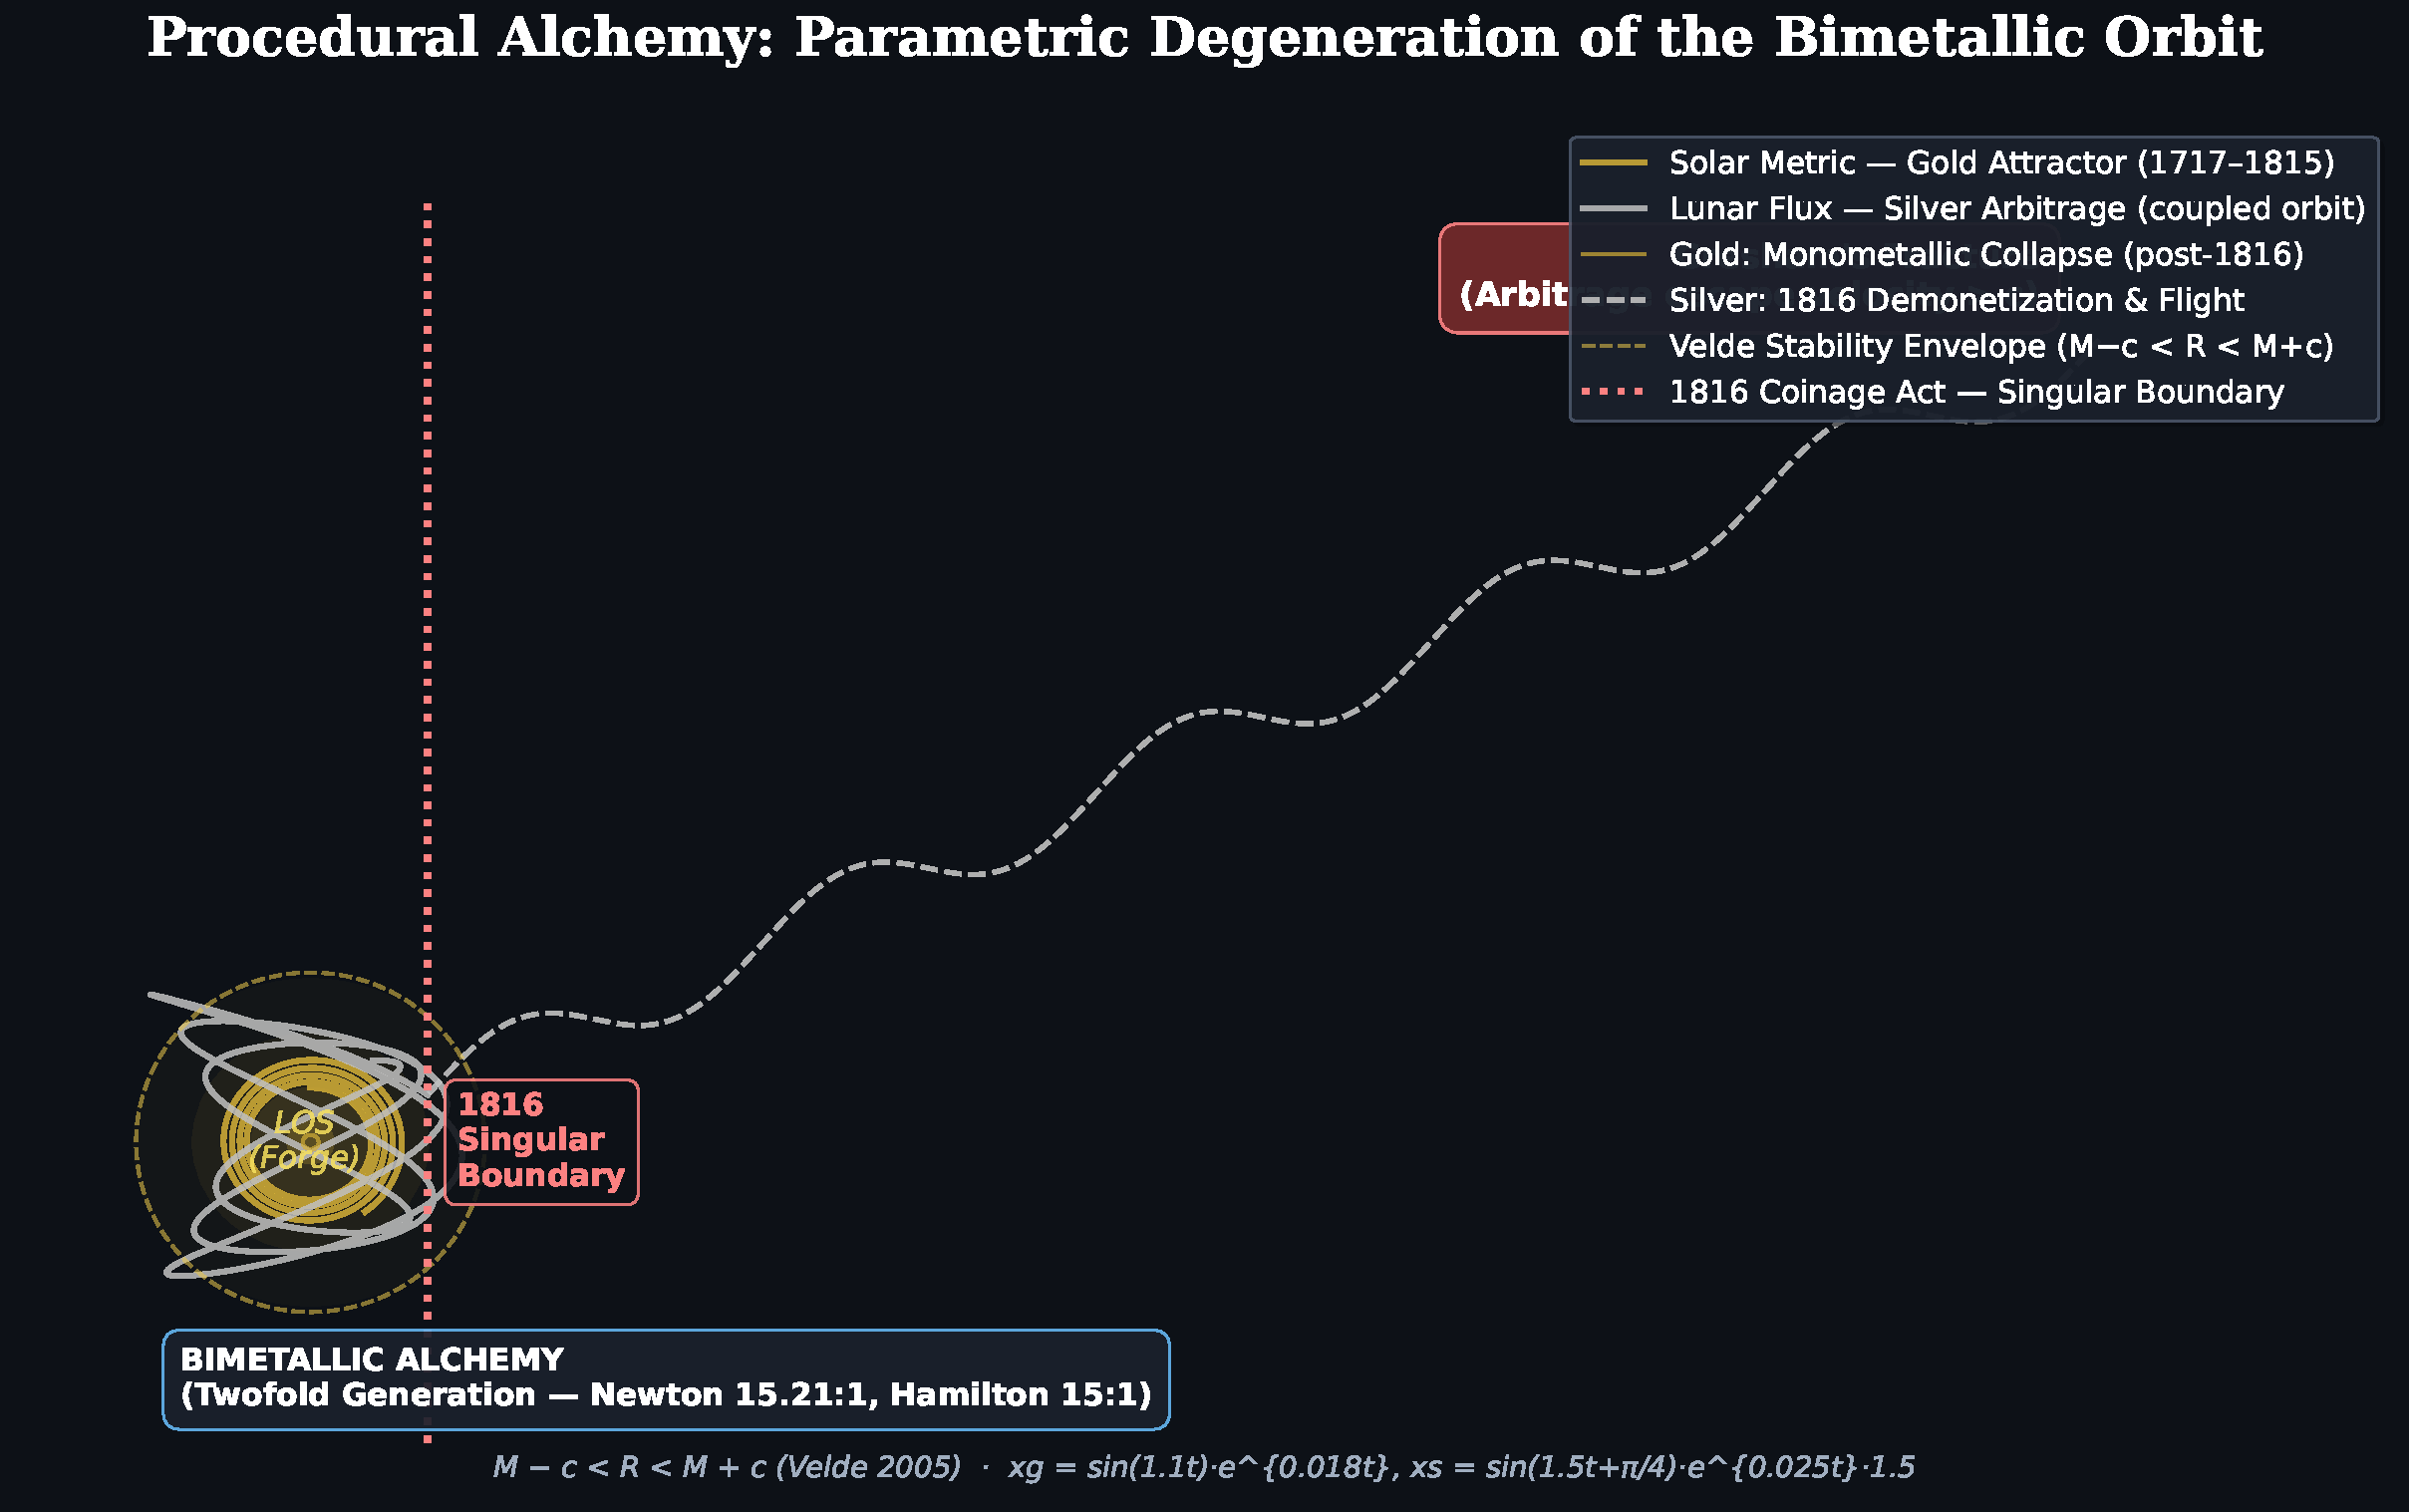
\includegraphics[keepaspectratio,alt={Procedural Alchemy of Bimetallic Vectors --- Parametric Degeneration of Bimetallic Orbit. This procedurally generated 5000-point Harmonograph maps the historical vectors of Solar Gold (the central, tight attractor) and Lunar Silver (the wider, sweeping orbit of the 1.5 ratio) locked in meta-stable Twofold Generation. Mathematical harmony holds until the Velde stability ellipse threshold is breached (R \textgreater{} M + c). At the 1816 singular boundary, Gresham's arbitrage escape velocity is crossed: the Solar Gold vector collapses inward to a static geometric dot at the Urizen pole (Single Vision / The Gold Standard with 4-layer glow rings), while the Lunar Silver vector violently breaks orbit toward the Los pole, escaping tangentially into chaotic space---modeling the physical demonetization of silver under the Coinage Act (56 Geo. III c.68) and the total eradication of the bimetallic generative synthesis. Includes the parametric equation xg = \textbackslash sin(1.1t)e\^{}\{0.018t\}, xs = \textbackslash sin(1.5t+\textbackslash pi/4)e\^{}\{0.025t\} \textbackslash cdot 1.5.}]{../figures/alchemical_bimetallism_dark.pdf}}
\caption{Procedural Alchemy of Bimetallic Vectors --- Parametric
Degeneration of Bimetallic Orbit. This procedurally generated 5000-point
Harmonograph maps the historical vectors of Solar Gold (the central,
tight attractor) and Lunar Silver (the wider, sweeping orbit of the 1.5
ratio) locked in meta-stable Twofold Generation. Mathematical harmony
holds until the Velde stability ellipse threshold is breached
(\(R > M + c\)). At the 1816 singular boundary, Gresham's arbitrage
escape velocity is crossed: the Solar Gold vector collapses inward to a
static geometric dot at the Urizen pole (Single Vision / The Gold
Standard with 4-layer glow rings), while the Lunar Silver vector
violently breaks orbit toward the Los pole, escaping tangentially into
chaotic space---modeling the physical demonetization of silver under the
Coinage Act (56 Geo. III c.68) and the total eradication of the
bimetallic generative synthesis. Includes the parametric equation
\(xg = \sin(1.1t)e^{0.018t}, xs = \sin(1.5t+\pi/4)e^{0.025t} \cdot 1.5\).}\label{fig-alchemy}
\end{figure}

\newpage

\section{The 1797 Bank Restriction and the Suspension of Metallic
Reality}\label{sec-bank-restriction-1797}

The meta-stable tension of Twofold bimetallism finally shattered under
the geopolitical pressures of the French Revolutionary Wars. By the late
1790s, Britain was facing a multidimensional crisis of liquidity,
sovereignty, and national survival. Panic swept the countryside as
rumors of French invasion---dramatically realized by the Battle of
Fishguard (22--24 February 1797), the last foreign invasion force to
land on British soil---prompted local farmers and mercantilists to storm
the provincial banks, demanding hard gold for their paper notes. These
localized runs cascaded into Threadneedle Street.

By the end of February 1797, the Bank of England's gold reserves had
dwindled to critical levels---roughly £1.1 million against total note
circulation of just over £10.8 million, meaning the face value of paper
in circulation was nearly twice the actual bullion held
\citep{clapham1944bank}. The Bank's reserves had declined by £622,000
since 1 January alone, a depletion rate that threatened institutional
collapse within days. Fearing a dissolution of the imperial treasury,
the Privy Council issued its emergency order on 26 February 1797
(Saturday evening, with notification reaching the Bank by Sunday
morning), which was formalized by Parliament as the Bank Restriction Act
(37 Geo. III c.45), receiving Royal Assent on 3 May 1797
\citep{fetter1965development}. This legislation legally suspended the
convertibility of Bank of England notes into gold specie. The physical,
elemental anchor of British wealth was severed overnight; the state was
now legally empowered to print value \emph{ex nihilo}
\citep{ricardo1810high}.

\subsection{The Atomic Swerve: Fiat Currency and Forgery's Media
Ecology}\label{the-atomic-swerve-fiat-currency-and-forgerys-media-ecology}

This suspension unleashed an era of unbacked, proliferating paper
currency that persisted until 1821. In the schema of Blakean and
Epicurean philosophy, the 1797 suspension represents the historical
manifestation of the atomic \emph{clinamen}---the swerve of value away
from metal. Unmoored from its metallic gravity, value swerved wildly.
Threadneedle Street flooded the economy with low-denomination £1 and £2
notes to replace hoarded gold, relying on crude mass-printing that was
trivially easy to counterfeit.

As Saree Makdisi argues, this deluge radically reshaped London's ``media
ecology'' \citep{makdisi2003william}. Paper money ceased to be an elite
mercantile instrument and became a ubiquitous social contagion among the
poor. When Blake writes of ``mind-forg'd manacles'' in \emph{London}
(1794), he is diagnosing the very ideological enclosure that William
Pitt's paper-funded war machine would soon legally enforce: the working
classes were trading their labor for ``allegoric riches,'' paper claims
that promised value while systematically stripping it away through
inflation.

Crucially, Blake's philosophical hatred of this ``spectral value''
crystallized through documented, artisanal confrontation with the Bank.
On 5 April 1797---mere weeks after the suspension---William Blake joined
18 prominent London engravers in signing a formal certificate endorsing
Alexander Tilloch's revolutionary ``stereotype'' method for producing
forge-proof banknotes. (Though occasionally conflated with the
commercial ``writing engraver'' W.S. Blake, the poet's presence among
his guild peers on this petition is established in the primary record
preserved in G.E. Bentley Jr.'s \emph{Blake Records}
\citep{bentley2004records}). The historical irony is profound: the
visionary who most despised ``allegoric riches'' sought to protect them
from forgery, not out of love for the Bank, but through an artisan's
commitment to high-fidelity, irreproducible craft. The Bank's
Directorate rejected Tilloch's solution. The immediate consequence of
this Urizenic choice was a precipitous spike in counterfeiting, which
the state answered with mass hangings. For Blake, the Bank's paper money
was not merely an economic abstraction; its defense literally demanded
human sacrifice. The poorest of London were executed to protect the
Bank's groundless, easily forged monopoly
\citep{baucom2005specters, erdman1954prophet, crosby2011blake}.

Blake had prophetically dramatized precisely this dissolution of
metallic anchor in \emph{Europe A Prophecy} (1794), etched just three
years before the Restriction. In that poem, Enitharmon---the emanation
of Los, Blake's spirit of sensuous beauty and deceptive
repose---commands an eighteen-hundred-year ``golden night'' of spiritual
slumber: ``Now comes the night of Enitharmon's joy! / Who shall I call?
Who shall I send? / That Woman, lovely Woman! may have dominion?''
(Plate 5, lines 1--3; Erdman p.~63) \citep{erdman1988complete}. This
``golden night'' is Blake's image for the enchantment of material
seeming---a false golden age sustained not by authentic metallic
substance but by the seductive illusion of value. When Enitharmon's
night shatters at the poem's climax with the trumpet of revolution, the
parallel to the Restriction is exact: the ``golden'' currency regime
collapses, revealing that its supposed solidity was always an
enchantment sustained by sovereign fiat rather than intrinsic worth.

Henry Thornton's landmark \emph{An Enquiry into the Nature and Effects
of the Paper Credit of Great Britain} (1802) documented this credit
crisis with analytical precision, demonstrating how the expansion of
paper credit operated independently of any metallic constraint and
thereby introduced radical instability into the pricing of commodities
\citep{thornton1802nature}. The everyday economy, once rooted in the
physical weight of the harvest and the hand, metamorphosed into a
circulation of purely relational symbols. It became a linguistic rather
than a substantive economy---a highly effective iteration of Urizenic
abstraction.

\begin{figure}
\centering
\pandocbounded{\includegraphics[keepaspectratio,alt={The Flight of Credit --- Bank of England Note Issuance vs.~Physical Gold Reserves (1790--1821). Top panel: visualizes the profound ontological gap emerging during the Bank Restriction period---skyrocketing issuance of fictional paper credit (``allegoric riches,'' £M) against drained physical gold reserves (£M). Vertical dashed lines mark the catastrophic date of 26 February 1797 (Privy Council suspended specie payments with reserves at roughly £1.1 million), the 1816 Coinage Act, and Peel's 1821 Resumption. The ``uncovered credit gap'' is shaded between notes and reserves. Bottom panel: the reserve coverage ratio plummets from \textasciitilde80\% before suspension to a nadir of \textasciitilde6.7\% in 1813, establishing the fiat void. Data derived from scholarly estimates of the restriction era {[}@clapham1944bank; @tooke1838history{]}.}]{../figures/historic_reserves_dark.pdf}}
\caption{The Flight of Credit --- Bank of England Note Issuance
vs.~Physical Gold Reserves (1790--1821). Top panel: visualizes the
profound ontological gap emerging during the Bank Restriction
period---skyrocketing issuance of fictional paper credit (``allegoric
riches,'' £M) against drained physical gold reserves (£M). Vertical
dashed lines mark the catastrophic date of 26 February 1797 (Privy
Council suspended specie payments with reserves at roughly £1.1
million), the 1816 Coinage Act, and Peel's 1821 Resumption. The
``uncovered credit gap'' is shaded between notes and reserves. Bottom
panel: the reserve coverage ratio plummets from \textasciitilde80\%
before suspension to a nadir of \textasciitilde6.7\% in 1813,
establishing the fiat void. Data derived from scholarly estimates of the
restriction era
\citep{clapham1944bank, tooke1838history}.}\label{fig-historic-reserves}
\end{figure}

\subsection{\texorpdfstring{Blake's \emph{Vala} and the Ontology of
Paper Credit: The Paper
Epic}{Blake's Vala and the Ontology of Paper Credit: The Paper Epic}}\label{blakes-vala-and-the-ontology-of-paper-credit-the-paper-epic}

Simultaneous to this financial \emph{clinamen}, William Blake commenced
organizing and writing his first sweeping epic prophecy, \emph{Vala, or
The Four Zoas} (1797--1807). Surrounded by the chaos of unbacked paper
abstraction in London, Blake articulated the nightmare of the
fragmented, alienated psyche corresponding to a fragmented, alienated
social body. The suspension of specie was not merely a fiscal mechanism
for Blake; it was a plunge into the depth of \textbf{Ulro}---the void of
single vision and spiritual death. Rather than entering the dream-like
poetic rest of Beulah, the economy sank into spectral abstraction, where
value became entirely disembodied from both Generative labor and
tangible reality. It was the Epicurean universe---ungrounded,
atomized---realized as policy. Patrick Brantlinger argues that the
establishment of the national debt and the proliferation of paper credit
effectively conjured ``fictions of state,'' turning the British empire
into an entity sustained entirely by future promises rather than
substantive present reality
\citep{brantlinger1996fictions, tooke1838history}. Ian Baucom extends
this critique in his study of finance capital and the Atlantic slave
trade, demonstrating how this era of British credit relied on an
epistemology of ``spectral value,'' wherein human life itself became
fully fungible and exchangeable on international ledgers
\citep{baucom2005specters}. It was the total atomization of social value
into swerving, groundless paper contracts, fractional reserve banking,
and what Blake elsewhere termed ``allegoric riches'' (Plate 27,
\emph{Jerusalem}) \citep{makdisi2003william, erdman1988complete}.

The Bank Restriction Act essentially created an environment where
private mercantile debt was transmuted into a public burden, tearing at
the fabric of social cohesion. As gold disappeared from
circulation---either hoarded domestically or shipped abroad---the
everyday citizen was forced to navigate the precarity of
small-denomination paper notes and degraded silver tokens. David
Ricardo's influential pamphlet \emph{The High Price of Bullion, a Proof
of the Depreciation of Bank Notes} (1810) crystallized the mounting
intellectual case against the Bank's profligacy, insisting that the
rising price of gold bullion was empirical proof of the depreciation of
paper---not, as the Bank's directors claimed, merely a symptom of
wartime scarcity \citep{ricardo1810high}. The resulting Bullionist
Controversy (explored in \hyperref[sec-bullionist-controversy]{§ The
Bullionist Controversy}) demanded a radical prophetic intervention to
restore meaning and value, while simultaneously setting the stage for
Urizen's eventual, systemic re-assertion of numerical containment in
1816. The period of Restriction (1797--1821) thus served as the chaotic
\emph{Ulro} out of which the repressive order of the Gold Standard would
be forged.

\newpage

\section{The Bullionist Controversy and the Semiotics of
Value}\label{sec-bullionist-controversy}

The aftermath of the 1797 Bank Restriction Act birthed the Bullionist
Controversy, a political and economic debate that raged throughout the
early 19th century and culminated in the 1810 Bullion Report presented
to Parliament. Crucially, this economic debate mapped closely onto the
semiotic and epistemological battles William Blake was waging in his
prophetic poetry. The central issue of the Controversy was whether the
rising price of bullion resulted from the over-issuance of paper money
(the ``Bullionist'' position), or if the paper money was maintaining its
value while gold itself was appreciating due to wartime scarcity (the
``Anti-Bullionist'' position) \citep{fetter1965development}.

\textbf{Bullionists (Ricardo and the metallic anchor).} The Bullionists,
led by figures like David Ricardo and embodied in the 1810 Bullion
Report, argued that value must refer back to a physical, metallic
anchor. Ricardo's \emph{The High Price of Bullion, a Proof of the
Depreciation of Bank Notes} (1810) provided the intellectual foundation:
the premium on gold bullion over the nominal value of banknotes
constituted empirical proof that the Bank had depreciated the currency
through overissuance \citep{ricardo1810high}. Henry Thornton, in his
\emph{An Enquiry into the Nature and Effects of the Paper Credit of
Great Britain} (1802), offered a more nuanced but equally comprehensive
analysis, demonstrating that the Bank's credit expansion operated with
radical independence from any metallic constraint, introducing systemic
instability into all commodity prices \citep{thornton1802nature}. For
the Bullionists, the post-1816 pound was effectively anchored to the
sovereign's 113 grains of fine gold, and any deviation from that anchor
was considered a species of national fraud.

\textbf{Anti-Bullionists (the Bank's directors).} The Anti-Bullionists,
representing the Bank of England's directors and their parliamentary
allies, paradoxically argued for a more abstract, relational conception
of value. They claimed that their paper notes represented not a fixed
weight of metal, but the ``needs of trade''---the aggregate commercial
demand of the nation. This was an early doctrine of paper credit and
convertibility: that the Bank's notes could circulate so long as
confidence and state backing sustained them
\citep{fetter1965development}. From the perspective of Blakean
cosmology, this Anti-Bullionist position occupied a sophisticated space:
it acknowledged the constructed nature of monetary value, but deployed
this acknowledgment to entrench the oligarchic power of the Bank's
governors rather than to liberate humanity from quantification.

\subsection{Blake's Refusal: Newton's Mint and Los's
Forge}\label{blakes-refusal-newtons-mint-and-loss-forge}

In this debate, Blake's position is complex and irreducible to either
camp; he frames the crisis not as macroeconomic policy, but as a
political theology pitting \textbf{Newton's Mint} against \textbf{Los's
Forge}. He was certainly not a Bullionist---he abhorred the ``chimeric
regime'' of the gold standard and the worship of the ``guinea'' as a
false idol, declaring in his marginalia to Reynolds that to a miser, ``a
guinea is more beautiful than the sun'' \citep{blake1808annotations}.
Yet, he was equally critical of the Anti-Bullionist reality: a financial
oligarchy manipulating abstract paper contracts (``allegoric riches'')
to extract real labor from the poor. \emph{Jerusalem} Plate 27 targets
that dual exploitation at length (see \hyperref[sec-allegoric-riches]{§
The fixing of labour and allegoric riches})
\citep{erdman1988complete, sklar2011blake}.

Both the Bullionists and the Anti-Bullionists were trapped in
\emph{Urizenic} logic. One worshipped the atomic, finite particle (the
gold coin); the other worshipped the algorithmic void of credit
(fractional reserve banking). Against both, Blake posited Los's Forge:
the imaginative, artisanal production of eternal forms through immediate
physical labor. The material toll of this macroeconomic abstraction on
Los's Forge was substantive. As the Restriction era dragged on, the
economic pressures of currency instability and inflation severed the
working classes from the means of artistic production. By 1818,
overwhelmed by this fiat malaise, Blake virtually ceased printing his
illuminated books---producing only 14 copies of four titles
post-1795---and pivoted to commercial graphic art to survive
\citep{makdisi2003william}. The abstract ledgers of Threadneedle Street
had literally cooled the fires of the prophetic forge.

Blake's \emph{Fourfold Vision} (detailed under
\hyperref[sec-urizenic-materialism]{§ Urizenic materialism}) entirely
circumvents this dichotomy. For Blake, true value is not found in the
metallic anchor nor in the abstract paper calculus, but in the
generative, qualitative labor of the human imagination. The Bullionist
Controversy represented the ultimate crisis of capitalist semiotics
\citep{fetter1965development}---a society arguing over whether the
\emph{sign} (paper) should be bound to the \emph{referent} (gold), while
entirely ignoring the \emph{creator} of value (the human
artist/laborer). As Mary Poovey demonstrates in her analysis of ``genres
of the credit economy,'' the entire semiotic infrastructure of
eighteenth-century finance was built upon an irresolvable tension
between the promise of face value and the reality of market value---a
tension that Blake's prophetic works expose as symptomatic of the deeper
spiritual crisis of quantification itself \citep{poovey2008genres}. The
Controversy was eventually decided not by intellectual resolution but by
legislative force. Parliament had already codified gold-centred coinage
and token silver during Restriction in the \textbf{1816} Coinage Act
\citep{redish1990evolution}; \textbf{Peel's Act} of \textbf{1819} then
committed Britain to \textbf{resumption} of Bank-note convertibility
into specie by \textbf{1821}, closing the twenty-four-year arc of the
Restriction period \citep{fetter1965development} and binding the
restored metallic order to that statutory frame.

\newpage

\section{The Mythopoetics of Global Valuation: Los Against Urizenic
Materialism}\label{the-mythopoetics-of-global-valuation-los-against-urizenic-materialism}

\subsection{Urizenic Materialism and the Generation of ``Allegoric
Riches''}\label{sec-urizenic-materialism}

To counter the chaotic flux of paper abstraction and the arbitrage
strain of bimetallism, Urizen superimposes geometric limit. In Blake's
mythology, Urizen (often derived from ``Your Reason'' or the Greek
\emph{horizein}, ``to limit'') is the architect of the fallen material
world. Erdman's reading of Urizen as the ``great Work master'' and of
``slave labor'' as war finance, reserves, and commodified human energy
was established in our Introduction \citep{erdman1954prophet}. Saree
Makdisi extends this reading, positioning Blake as an anti-capitalist
who rejected the entire framework of commodity exchange, rational
calculation, and empire-driven trade as a ``flattening'' of human
existence \citep{makdisi2003william}.

Urizen's mathematically segmented universe mirrors the division of labor
that alienated the 18th-century worker from the product of their hands.
E.P. Thompson extends this analysis via his seminal reading of the poem
\emph{London}, interpreting the ``mind-forg'd manacles'' (line 8; Erdman
p.~70) as literal mechanical mechanisms of market alienation imposed by
the expanding, quantifying logic of industrial capitalism
\citep{thompson1993witness}. Thompson's critical intervention
demonstrates how Blake's deliberate imagery systematically indicts the
acquisitive ethic: dividing people, enforcing moral bondage, destroying
joy, and leading to death---all consequences of the reduction of human
life to labor-power exchangeable on the open market. This segmentation
of experience inherently relies upon the materialist reduction of
infinite, qualitative spiritual essence into calculable physical
vessels.

Blake's annotations to Francis Bacon's \emph{Essays Moral, Economical,
and Political} (c.~1798) contain his most concentrated marginalia
against the mercantile worldview. Where Bacon recommended ``the opening
and well balancing of trade; the cherishing of manufactures; the
banishing of idleness'' as prescriptions for national prosperity, Blake
dismissed the entire collection as ``Good advice for Satan's kingdom''
\citep{erdman1988complete}. More substantively, in response to Bacon's
axiom that national wealth is necessarily extracted from foreign
loss---``whatsoever is somewhere gotten is somewhere lost''---Blake
annotated: ``Bacon's Philosophy has Ruin'd England.'' This zero-sum
mercantile logic is precisely the Urizenic worldview that undergirds the
bimetallic system: wealth conceived not as qualitative human flourishing
but as a fixed quantum of metal to be captured through competitive
extraction.

Blake interrogates this exact ontological dynamic via the bimetallic
dualism in \emph{The Book of Thel} (1789):

\begin{quote}
``Can Wisdom be put in a silver rod? Or Love in a golden bowl?''
(\emph{The Book of Thel}, 1789) \citep{blake1789thel}
\end{quote}

By trapping infinite qualitative attributes (Lunar Wisdom and Solar
Love) into standardized, quantified containers (monetary Silver Rods and
Golden Bowls), the Urizenic state ensures only violent limitation. It is
the poetic expression of Gresham's Law and its underlying arbitrage
boundary: the rod and the bowl are not merely metaphors for human
experience, but precise alchemical designations for the two metals whose
statutory relationship governed the entire British monetary system. The
silver rod of Thel encodes the very silver coinage whose flight from
England---melted and shipped to France and India by the East India
Company---destabilized the fragile bimetallic synthesis. The golden bowl
encodes the hoarded, static gold that Newton's 1717 Mint ratio
artificially elevated above its natural equilibrium. Against this
quantification, Blake arrayed his revolutionary figure of Orc. Often
depicted metaphorically as a pillar of fire or a cosmic serpent, Orc
embodies the raw, unmeasured energy of human passion rising up against
the totalizing theocracy of Urizenic law---a fiery rejection of the
predictability and geometric constraint demanded by the gold standard
bureaucracy.

\subsection{The Fixing of Labour and the Invention of Allegoric
Riches}\label{sec-allegoric-riches}

The attempt to fix fluctuating, living subjective value within the
state-mandated algorithmic bounds of the Mint ratio inherently evacuates
the divine meaning of human existence. Blake recognized that the
creation of the modern banking system, the issuance of state debt, and
the fractional generation of credit was an act of misguided alchemy. In
\emph{Jerusalem} (Plate 27, lines 10--14), Blake explicitly targets the
architects of this macroeconomic enclosure:

\begin{quote}
``Shall not the Councellor throw his curb Of Poverty on the laborious?
To fix the price of labour; To invent allegoric riches.'' (Erdman
p.~169) \citep{erdman1988complete, sklar2011blake}
\end{quote}

As Susanne Sklar and modern scholars note, ``allegoric riches'' is a
profound critique of credit creation \emph{ex nihilo}. The Bank of
England held finite gold reserves---by 1797, roughly £1.1 million---but
issued paper credit exceeding £10 million, creating a vast
superstructure of fictional wealth \citep{clapham1944bank}. This
``allegoric'' system simultaneously enslaved the laboring class to
compounding debt while enriching a monopolistic financial elite who
controlled the issuance of the currency. Blake's phrase anticipates the
modern critique of central banking's capacity to create money through
lending, generating ``allegoric'' claims upon future production that
bear no necessary relationship to present reality. This materialist
mechanics maps directly onto Blake's ultimate villain: the rigid,
exploitative isolation of the \emph{Selfhood}
\citep{schouten2021lucretius}. To accept Urizen's economy is to accept a
world where the living pulse of humanity is subjugated to
quantification.

\subsection{Entering the Mathematical and Ontological Void of Paper
Credit}\label{entering-the-mathematical-and-ontological-void-of-paper-credit}

The transition from classical bimetallic friction to the 1797 paper
suspension catalyzed an ontological crisis that Blake internalized into
his epic structures. While gold and silver were idolized as ``Gods of
the Earth,'' paper credit was something even more destabilizing: it was
a pure, systemic void. It substituted verifiable human labor and scarce
elemental reality with infinite, self-referential debt obligations.
\emph{Vala, or The Four Zoas} (c.~1797), drafted as the Restriction
crisis broke, is haunted by this paper deluge. These spectral geometries
evoked new folkloric realities on the streets of London, most notably
the legend of the ``Bank Nun'' (Sarah Whitehead), whose brother Philip
Whitehead was convicted and executed for forging Bank of England notes
during the Restriction years. Driven mad by the state's lethal defense
of its fictional paper, Sarah arrived at Threadneedle Street daily for
over twenty-five years, dressed in black, demanding her brother's
return. For Blake, this intertwining of state execution and fiat forgery
was not merely socio-economic tragedy; it was the literal realization of
his mythological terror---the spectral economies of Urizen plagiarized
into living folk memory \citep{makdisi2003william}.

As Ian Baucom illuminates in his study of finance capital and the
Atlantic slave trade, this era of British credit relied on an
epistemology of ``spectral value,'' wherein human life itself became
fully fungible and exchangeable on international ledgers
\citep{baucom2005specters}. The speculative instruments of the City of
London---bills of exchange, promissory notes, treasury
bonds---constituted an entirely new semiotic regime in which the
\emph{sign} had been decisively severed from any \emph{referent},
floating freely in recursive financial self-reference without a stable
referent.

Alexander Regier argues that this new financial regime operated via
``fragmentation''---the deliberate shattering of the social contract
into isolated, competing financial claims that could be manipulated by
the state \citep{regier2010fragmentation}. If gold was the weight of
Urizen's geometry, paper credit was the abyss of Urizen's chaos. It
created an environment where the ``price of labor'' (Blake's exact
phrase from \emph{Jerusalem} Plate 27) was unmoored from reality,
subject entirely to the inflationary whims of the Bank. For Blake,
returning to metallic standards (the 1816 Coinage Act) was a regression
into tyranny, but accepting unbacked paper without limit was equally
disastrous. The only path forward was transcendence of both quantitative
regimes through imaginative creation---Los's refusal to be enslaved by
another's system (\emph{Jerusalem}, Plate 10)
\citep{erdman1988complete}, developed in
\hyperref[sec-four-levels-vision]{§ Fourfold Vision}.

\newpage

\section{Los, the Fourfold, and the Monetary
Arc}\label{los-the-fourfold-and-the-monetary-arc}

\subsection{Blake's Fourfold Vision and the Scales of Monetary
Generation}\label{sec-four-levels-vision}

Blake maps this escalating socioeconomic and spiritual entropy against
his definitive epistemological concept: the \textbf{Fourfold Vision}.
This paradigm directly traces the evolution of British monetary
architectures, moving from calculation, through generative (but
unstable) tension, to the ultimate requirement for an overarching
qualitative human integration (as explored further under
\hyperref[sec-illuminated-nonduality]{§ Illuminated Nonduality}).
Northrop Frye's foundational elucidation in \emph{Fearful Symmetry}
(1947) establishes that Blake's Fourfold Vision represents not merely a
poetic conceit but a complete philosophical telos: imaginative
creativity operating as a living, breathing power that restores the
fractured human form \citep{frye1947fearful}.

\subsubsection{Single Vision of Ulro: Atomized Monometallism and Fiat
Currency}\label{single-vision-of-ulro-atomized-monometallism-and-fiat-currency}

The lowest perceptual state in Blake's cosmology is \textbf{Ulro}
(\emph{Single Vision}). Dominated strictly by empirical measurement and
atomistic isolation, it is a realm of spiritual death---what Blake
describes as ``Newtons sleep,'' the stupor of pure quantification. As
Susanne Sklar notes, ``In Ulro, that which can't be expressed
quantitatively does not exist'' \citep{sklar2011blake}. In monetary
mechanics, \emph{Single Vision} equates identically to strict
Monometallism---the Urizenic fetishization of a single currency vector
(Gold) serving as an inflexible standard (see the 1816 Regression in
\hyperref[sec-coinage-act-1816]{§ The 1816 Coinage Act}). The 1816
Coinage Act, which legally restricted silver to token coinage with a
40-shilling legal tender limit, constitutes the legislative realization
of Ulro: the elimination of duality and generative tension in favor of a
monistic, reductionist finality. Ulro is also the state of unbacked fiat
paper from 1797---a disconnected void where the Bank of England's notes,
backed by reserves of roughly £1.1 million against over £10 million in
circulation, constituted a semiotic void \citep{clapham1944bank}. It
enforces total reductionism, severing spiritual context and dismissing
any human value that cannot be weighed on capitalist scales or entered
into a ledger.

\subsubsection{Twofold Vision of Generation: The Dialectic of Structural
Bimetallism}\label{twofold-vision-of-generation-the-dialectic-of-structural-bimetallism}

Escaping the void of Ulro leads to \textbf{Generation} (\emph{Twofold
Vision}). As documented, the Bimetallic standard is the historical
instantiation of Twofold Vision (see \hyperref[fig-alchemy]{the
Harmonograph}). It is a realm of biological and economic reproduction,
deeply meta-stable, and prone to the unceasing arbitrage of Gresham's
Law. Importantly, the crisis of bimetallic arbitrage was not a failure
of Twofold integration itself; it was the inevitable rupture caused by
attempting to govern a living, dual system with the rigid mathematics of
\emph{Single Vision} (Newton's immutable Mint Ratio). Single Vision
cannot permanently bind dynamic dualities. Yet, as Buckminster Fuller
would assert in \emph{Synergetics}, ``Unity is plural and, at minimum,
two'' \citep{fuller1975synergetics}---a structural necessity Blake
anticipated through his defense of Generative tension. Minimum two
provides the resilient platform required to enter into Threefold and
Fourfold qualification. It is a site of suffering and labor, but
nevertheless a vastly superior state to Ulro: it acknowledges duality,
tension, and relative interaction over the violence of geometric
singularity or monometallic fiat. Silver and Gold exist in a dynamic,
albeit precarious, relationship---bound by Newton's 1:15.21 ratio yet
perpetually strained by international market forces that valued silver
more highly abroad. This is the productive but agonizing state of human
existence: the alchemical marriage of Sol and Luna that Del Mar
identifies as the sacred foundation of all legitimate coinage
\citep{delmar1895history}. The instability is not a flaw but a
feature---it is the generative friction of two irreducible principles in
dialogue, the very condition of creative evolution.

\subsubsection{Threefold Vision of Beulah: The Affective and
Psychological
Threshold}\label{threefold-vision-of-beulah-the-affective-and-psychological-threshold}

Above Generation lies \textbf{Beulah} (\emph{Threefold Vision}), the
realm of emotional insight and intuitive apprehension. In monetary
terms, Beulah represents the fleeting historical moments when economic
policy briefly served human flourishing rather than extractive
accumulation---periods of relative prosperity and social cohesion that
exist precariously between the grinding mechanisms of Urizenic finance.
Beulah is, in Blake's cosmology, a necessary way-station, a ``married
land'' of rest and restoration, but one that cannot sustain itself
indefinitely without ascending into the full creative synthesis of Eden.

\subsubsection{Fourfold Vision of Eden: The Ultimate Prophetic Monetary
Assertion}\label{fourfold-vision-of-eden-the-ultimate-prophetic-monetary-assertion}

In \emph{Jerusalem}, the prophetic artisan Los rejects both the void of
Ulro and the mere passive calculation of financial ratios found in
Generation (the 1-fold and 2-fold quantification) with an operational
doctrine:

\begin{quote}
``I must Create a System, or be enslav'd by another Mans / I will not
Reason \& Compare: my business is to Create'' (\emph{Jerusalem}, Plate
10, lines 20--21; Erdman p.~153) \citep{erdman1988complete}
\end{quote}

This decree is a direct philosophical rebuff to the bimetallic
arbitrageur who exists only to ``Reason \& Compare'' the Gresham Entropy
Gap---calculating the exact moment when the silver-to-gold ratio across
the channel offers a risk-free margin. It is also, at a generic level, a
rejection of the foundational axiom of classical political economy: that
rational self-interest, expressed through price signals and arbitrage,
constitutes the highest form of social coordination. Blake insists that
the \emph{minute particular}---the irreducible, non-fungible quality of
individual human experience---cannot be captured by any system of
relative prices. As Makdisi argues, Blake's anti-capitalism is not a
sentimental nostalgia for pre-industrial life but a rigorous,
philosophically grounded rejection of the entire framework of commodity
exchange \citep{makdisi2003william}. Through Los's roaring furnaces,
Blake asserts the absolute necessity of advancing beyond quantitative
mechanics. He demands a leap into the qualitative synthesis of the
\emph{Threefold} (emotional/affectionate) and \emph{Fourfold}
(Edenic/imaginative) states, where real value is birthed in artistic and
spiritual creation rather than through financial extraction.

\begin{figure}
\centering
\pandocbounded{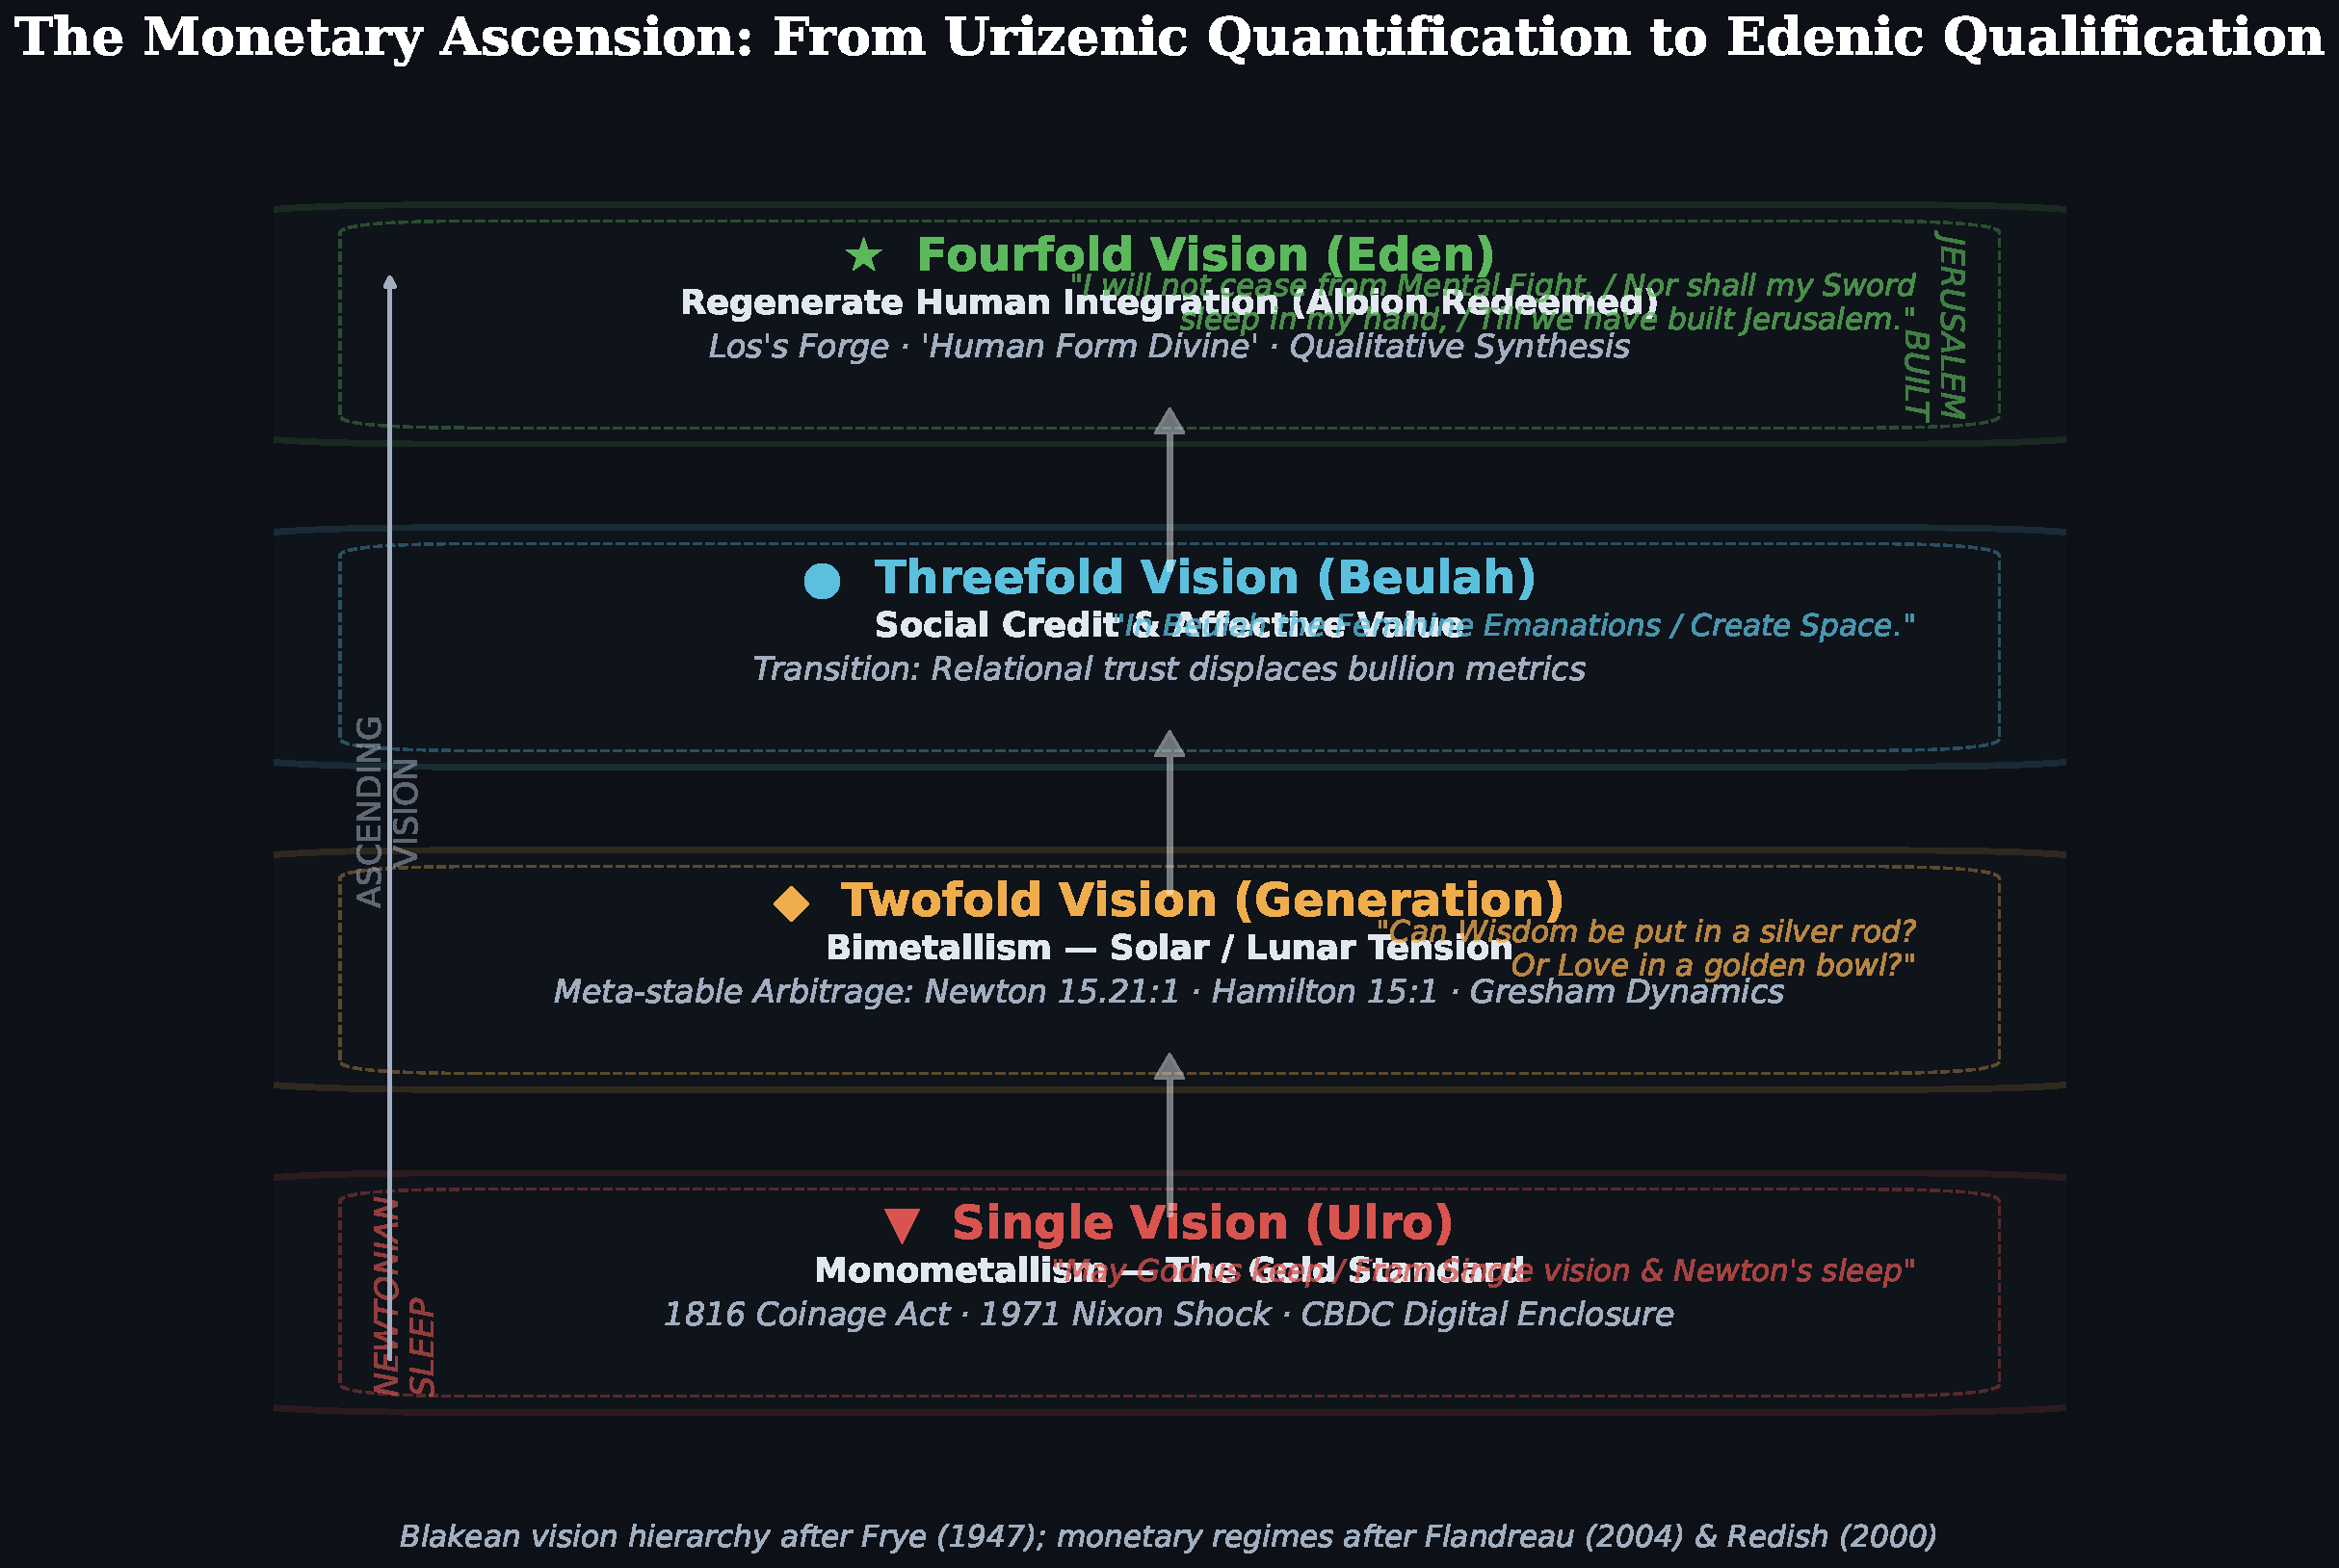
\includegraphics[keepaspectratio,alt={The Monetary Ascension --- From Ulro to Eden. A four-tiered ontological mapping elevating from the reductionist Monometallic standard of Ulro (Single Vision) through the generative bimetallic tension of Generation (Twofold Vision), the affective threshold of Beulah (Threefold Vision), and culminating in the non-dual qualitative integration of the Edenic state (Fourfold Vision). Each tier maps directly onto a specific historical monetary regime, from the sterile finality of the 1816 Gold Standard and modern CBDC digital enclosure (Ulro) to the visionary artisanal economics embodied in Los's forge (Eden). The visualization juxtaposes these monetary systems with direct Blakean poetic quotations for each level. This progression provides a critical topological heuristic for reading Blake's late epics: the journey out of the fallen world is not an escape from materiality, but an ascension through increasingly complex architectures of socio-economic relationality.}]{../figures/fourfold_mapping_dark.pdf}}
\caption{The Monetary Ascension --- From Ulro to Eden. A four-tiered
ontological mapping elevating from the reductionist Monometallic
standard of Ulro (Single Vision) through the generative bimetallic
tension of Generation (Twofold Vision), the affective threshold of
Beulah (Threefold Vision), and culminating in the non-dual qualitative
integration of the Edenic state (Fourfold Vision). Each tier maps
directly onto a specific historical monetary regime, from the sterile
finality of the 1816 Gold Standard and modern CBDC digital enclosure
(Ulro) to the visionary artisanal economics embodied in Los's forge
(Eden). The visualization juxtaposes these monetary systems with direct
Blakean poetic quotations for each level. This progression provides a
critical topological heuristic for reading Blake's late epics: the
journey out of the fallen world is not an escape from materiality, but
an ascension through increasingly complex architectures of
socio-economic relationality.}\label{fig-fourfold}
\end{figure}

\newpage

\section{The Alchemical Forges: Los vs.~The Royal
Mint}\label{the-alchemical-forges-los-vs.-the-royal-mint}

If Urizen is the bureaucratic Master of the Mint---the Newtonian
administrator calculating ratios, imposing geometric limits, and
standardizing the infinite human soul into weighed coins---then Los is
the divine blacksmith, the alchemist of the spirit. The opposition
between these two figures encodes one of the most structurally coherent
economic critiques in the entire Romantic canon.

\subsection{The Mint on Tower Hill: Engines of
Homogenization}\label{the-mint-on-tower-hill-engines-of-homogenization}

In \emph{Jerusalem}, Los is constantly depicted laboring at his roaring
furnaces. Blake utilizes explicitly metallurgical and alchemical imagery
to describe this work. However, whereas the Royal Mint on Tower Hill,
relocated in the early 19th century to a new purpose-built facility, was
an industrial fortress of steam-powered homogenization, Los's forges are
designed to produce living, differentiated, irreducibly unique human
forms (Eden). The Mint's industrial transformation was itself a symptom
of the Urizenic revolution: Matthew Boulton's steam-powered coining
presses, installed at the Soho Mint in Handsworth (near Birmingham) and
later adopted at the Royal Mint, could strike coins with mechanical
precision at high speed, eliminating the human hand from the minting
process entirely and replacing the artisan's judgment with calibrated,
replicable force.

The Mint melts down the various, chaotic silver and gold of the world
and stamps it with the sovereign's head---a singular image of authority.
It is a process of extraction and homogenization that parallels exactly
the Urizenic cosmogony described in \emph{The First Book of Urizen}
(1794), where the tyrant ``form'd golden compasses / And began to
explore the Abyss'' \citep{blake1794urizen}. Los's furnaces, conversely,
operate on a principle of spiritual alchemy: taking the fragmented,
degraded, atomic material of the fallen world and fusing it back
together through the heat of prophetic imagination into the ``Human Form
Divine.'' This opposition encodes a fundamental first-principles insight
into the nature of value itself: the Mint's operation is
\emph{subtractive} (reducing diverse human labor to a single metallic
denominator), whereas Los's forge is \emph{additive} (synthesizing
fragmented experience into integrated wholes).

The metallic imagery in \emph{Jerusalem} is pervasive and deliberate. On
Plate 12, Blake describes the spiritual architecture of
Golgonooza---Los's prophetic city, the anti-London---in explicitly
metallurgical terms:

\begin{quote}
``The stones are pity, and the bricks, well wrought affections, Enameld
with love \& kindness, \& the tiles engraven gold, Labour of merciful
hands: the beams \& rafters are forgiveness: The mortar \& cement of the
work, tears of honesty: the nails, And the screws \& iron braces, are
well wrought Blandishments'' (\emph{Jerusalem}, Plate 12, lines 30--34;
Erdman p.~155) \citep{erdman1988complete}
\end{quote}

Here the ``tiles engraven gold'' and ``iron braces'' serve a function
opposed to the Mint's gold: they are construction materials for a city
built from human affect---pity, kindness, forgiveness, honesty---rather
than the weight of bullion. Further, on the same plate, Blake names
``the golden Looms of Cathedron'' and ``the golden mills of Los'' (Plate
12, lines 46--47; Erdman p.~156), establishing that Los possesses his
own golden instruments, but ones devoted to weaving and milling the
fabric of human reality rather than stamping coins of abstract
equivalence. The adjective ``golden'' in Blake is thus bifurcated:
Urizen's gold is dead and hoarded; Los's gold is living, laboring, and
regenerative.

Crucially, on Plate 13, Blake extends this metallurgical architecture of
Golgonooza to enumerate the four metals of its gates in direct
correspondence with the Fourfold Vision:

\begin{quote}
``And that toward Eden, four, form'd of gold, silver, brass, \& iron.
The South, a golden Gate, has four Lions terrible, living! That toward
Generation, four, of iron carv'd wondrous: That toward Ulro, four, clay
bak'd, laborious workmanship That toward Eden, four; immortal gold,
silver, brass \& iron.'' (\emph{Jerusalem}, Plate 13; Erdman p.~157)
\citep{erdman1988complete}
\end{quote}

The sequence---gold, silver, brass, iron---is not arbitrary decoration.
It encodes a precise descending hierarchy of spiritual states, from
Edenic gold (imaginative fullness) through silver (generative Beulah,
the lunar-feminine, the bimetallic) and brass (the passionate-Orcian)
down to iron (the Urizenic-rational) and finally clay (Ulro, the void of
pure materialism). Silver occupies the second position in this sequence:
it is the metal of \emph{Beulah}, the intermediate state of rest and
generation, the lunar complement to the solar gold of Eden. This
structural placement is the most precise confirmation in the entire
Blakean corpus that silver, when paired with gold, represents
\emph{Generation}---the very bimetallic synthesis whose legislative
elimination in 1816 Blake's prophetic work condemned. Blake's Golgonooza
literalizes the four metals of the bimetallic tradition into a
cosmological architecture, with silver as the load-bearing structural
element between Eden and the fallen world.

\subsection{The Boulton Press and the Division of the Artist's
Body}\label{the-boulton-press-and-the-division-of-the-artists-body}

Blake explicitly contrasts the mechanical, steam-powered presses of
early industrial capitalism---embodied most visibly by the Boulton steam
presses---with the vital, bodily labor of the artist. The production of
true value requires sweat, breath, and the integrated labor of the
entire human body, not the alienated pull of a lever. As Thompson
documents, Blake's hostility to industrial machinery was not Luddite
nostalgia but a precise philosophical objection: the machine severs the
connection between the laborer's creative will and the product of their
hands, reproducing the structure of Urizenic alienation at the level of
daily lived experience \citep{thompson1993witness}.

\begin{quote}
``And Los's Furnaces howl loud; living: self-moving: lamenting With Fury
\& Despair, \& they dictate the relations of States'' (\emph{Jerusalem},
Plate 73) \citep{erdman1988complete}
\end{quote}

The furnaces are not inert mechanisms; they are \emph{living},
\emph{self-moving}, \emph{lamenting}---they participate in the suffering
of the human condition even as they labor to transcend it. This is
Blake's radical proposition: that the sites of genuine
production---artistic, spiritual, political---are necessarily sites of
anguish and fury, not the automated efficiency of the Mint.

\subsection{The Anti-Coin: Blake's Illuminated Printing as Economic
Subversion}\label{the-anti-coin-blakes-illuminated-printing-as-economic-subversion}

For Blake, the true economy is not dictated by the Bank of England or
the bullion brokers of the Royal Exchange, but by the ``Furnaces of
Los.'' Relief-etching inverts the Mint's stamping dies: where the
\textbf{Great Recoinage} (1696--1699), under Newton's Wardenship,
\emph{stamped} sovereign authority onto discs to impose fungible value,
and the \textbf{1717} guinea valuation later fixed the gold--silver
ratio, Blake \emph{dissolved} copper in acid to yield plates that resist
fungible exchange \citep{poovey2008genres}. The full phenomenology of
the anti-coin---\emph{Marriage of Heaven and Hell}, infernal method,
nondual matrix, division of labor, and \emph{Milton}'s injunction
against counting gold---is developed under
\hyperref[sec-illuminated-nonduality]{§ Illuminated Nonduality}.

The choice facing humanity is clear: be minted as a passive coin under
Urizen, or forge one's own infinite value in the roaring fires of Los
\citep{blake1804jerusalem}. As Erdman argues, this is not merely
artistic preference but political economy: Blake's mode of production
constitutes a complete alternative to the industrial system, one in
which the producer retains full sovereignty over the means, process, and
meaning of their labor \citep{erdman1954prophet}.

\newpage

\section{Quantification into Qualification: From Mint Metrics to
Fourfold
Measure}\label{quantification-into-qualification-from-mint-metrics-to-fourfold-measure}

\subsection{Illuminated Nonduality and the Cultivation of the Fourfold
Vision}\label{sec-illuminated-nonduality}

Meta-stability inevitably ruptures, as demonstrated by the arbitrage of
Gresham's Law. But for Blake, rupture is not the end; it is the
threshold marking the transition from the tensions of \textbf{Generation
(Twofold Vision)} and \textbf{Beulah (Threefold Vision)} into the
liberation of \textbf{Eden (Fourfold Vision)}: the realization of the
``regenerate 4-fold man.''

This eschatological pivot demands the abandonment of Urizenic
\emph{Quantification} (see \hyperref[sec-four-levels-vision]{Fourfold
Vision}) in favor of infinite, boundless \emph{Qualification}. As
Northrop Frye elucidates in his foundational work \emph{Fearful
Symmetry}, Fourfold Vision represents Blake's ultimate philosophical and
spiritual telos: it is imaginative creativity operating as a living,
breathing power, restoring the fractured human form, Albion
\citep{frye1947fearful}. In Blake's mythology, Albion is simultaneously
the primal human, the island of Britain, and the totality of human
civilization---his restoration is therefore at once a personal,
political, and cosmic event. In a truly Fourfold economic system, value
is no longer an intrinsic elemental property mysteriously inhering in
dead base matter (like the weight of gold bullion in a bank vault) or
fictional ledgers of compounding usury. Value becomes exclusively an
emergent property of qualitative, active, synergetic human integration.
It exists strictly within the context of radical human engagement---what
Saree Makdisi characterizes as Blake's ``rewrite'' of the material
capitalist order \citep{makdisi2003william}.

\subsection{The Anti-Coin, Infernal Method, and Undivided Labor on the
Plate}\label{the-anti-coin-infernal-method-and-undivided-labor-on-the-plate}

This refusal of capitalist order is not merely thematic in Blake's work;
it is embedded in his very mode of production: illuminated printing. By
inventing and operating his hybrid form of relief etching---biting words
and images simultaneously into corrosive copper baths in a single,
nondual matrix---Blake physically achieved a Fourfold qualitative
synthesis in his own life. The copperplate becomes the anti-coin.
Whereas the Royal Mint stamps an image of state authority onto a blank
disc to impose monolithic, fungible value---a process accelerated to
industrial scale by Boulton's steam presses---Blake dissolved the blank
surface of the copper with acid to reveal a unique, irreproducible
spiritual topography. Each illuminated plate cost Blake not the weight
of its metal but the expenditure of his creative attention: hours of
drawing, writing, etching, printing, and hand-coloring that could never
be mechanically replicated.

The imaginative economy of that practice was already announced in
\textbf{\emph{The Marriage of Heaven and Hell}} (c.~1790--1793)
\citep{blake1790marriage, erdman1988complete}. There Blake insists that
\textbf{``Without Contraries is no progression''}---life itself is the
clash of energies, not the suppression of one pole by a moralized
other---and the \textbf{Proverbs of Hell} celebrate the productive,
excessive, bodily energies that polite ``angelic'' reason would bind or
forbid. This is not a brief for moral evil but for \textbf{making}: the
devil's party, in Blake's ironic theology, is the party of unexhausted
creation. Read alongside the monetary argument of this manuscript, that
pamphlet subverts the same moralized dualism that underwrites
\textbf{Single Vision}: one lawful numéraire, one authorized face, one
passive subject who receives value stamped from above. The diabolic
register is thus a mythic prefiguration of \textbf{Los's Forge} against
\textbf{Newton's Mint}---energetic, particular, and corrosive of fixed
surfaces, where the Mint stands for cooled, countable, state-legible
sameness (developed in the opposition of Los to Urizen and the Mint in
the sections above).

Blake names the technical corollary \textbf{printing in the infernal
method} in \emph{Marriage} (Plate 14 in standard facsimiles; see Erdman)
\citep{blake1790marriage, erdman1988complete}: a deliberate, manual,
acid-driven process in which apparent surface is eaten away so that
letter and design stand in relief for a single pull from the press.
\textbf{Infernal} here names not sin but \textbf{contact with
transformative depth}---the same metaphorics that tie hell to energy in
the \emph{Proverbs}. Against Mint \textbf{stamping} (fungible discs,
interchangeable by weight) and against the divided workshop (specialist
plate, specialist press, specialist binder), the infernal plate is
\textbf{author-integrated, process-heavy, and non-fungible}: each
impression remains tethered to Blake's hand and to variable finishing.
The anti-coin is therefore both a semiotic and a \textbf{technical}
refusal of the universal equivalent.

The illuminated book then fuses poetry (temporal), visual art (spatial),
and physical labor (sculptural etching) into a single artifact that
defies the Urizenic division of labor. As Thompson argues, the division
of labor was the central mechanism of industrial capitalism's alienation
of the worker, and Blake's illuminated printing constitutes a
deliberate, material refusal of this division
\citep{thompson1993witness}. Blake took disparate, base elements and
united them in an unstable medium that is sustained entirely by the
human attention and interaction of the reader, demanding active,
Fourfold engagement to decode its sprawling mythological architecture.
The reader of an illuminated book cannot be a passive consumer---the
text demands interpretive labor, visual attention, and imaginative
participation simultaneously. This is the economic logic of Eden applied
to the act of reading itself.

Blake proved, through the very medium of his craft, that true and
lasting value is generated not by the metallic anchor overseen by Sir
Isaac Newton, nor the ``allegoric riches'' of the Bank Restriction, but
by the ``regenerate 4-fold man'' acting in imaginative societal synergy.
Through relief etching, Blake literally minted a new currency of the
spirit, one essentially immune to the arbitrage pressures of the
bimetallic world. As Blake declares in \emph{Milton}: ``Leave counting
Gold \& diamonds, for Gods eye delights in thee'' (Plate 26, line 27;
Erdman p.~121) \citep{erdman1988complete}---the injunction to abandon
the dead metrics of Urizen in favor of the infinite valuations of the
divine imagination.

\newpage

\section{The 1816 Coinage Act as Topological
Regression}\label{sec-coinage-act-1816}

While Blake proposed a visionary resolution to the meta-stable friction
of Twofold Generation through infinite, Fourfold spiritual expansion,
the British state pursued the exact opposite trajectory. Reacting
against both the swerve of unbacked paper money (see
\hyperref[sec-bank-restriction-1797]{§ The 1797 Bank Restriction}) and
the arbitrage of the bullion trade, the government sought a rigid
anchor.

\subsection{Lord Liverpool's Act: The Legislative Architecture of
Monometallism}\label{lord-liverpools-act-the-legislative-architecture-of-monometallism}

Under the guidance of Lord Liverpool, Parliament passed the Coinage Act
of 1816 (56 Geo. III c.68) on \textbf{22 June 1816}, officially known as
``An Act to provide for a New Silver Coinage, and to regulate the
Currency of the Gold and Silver Coin of this Realm.'' This Act legally
demonetized full-bodied silver entirely as a standard of value. It
relegated silver to a mere token coinage---reduced in weight to 66
shillings per troy pound from the prior 62 shillings, and declared legal
tender only for amounts up to \textbf{40 shillings}---effectively ending
the bimetallic alchemical marriage of the previous centuries and
enforcing a strict \emph{de jure} Gold Standard
\citep{redish1990evolution}. The new gold sovereign was defined at
\textbf{123.274 grains} (7.988 grams) of standard \textbf{22-carat gold}
(91.67\% pure), with one troy pound of standard gold equivalent to
\textbf{£46 14s 6d} (44½ guineas). This sovereign coin would become the
foundation of British imperial finance for a century.

\subsection{The Mathematical and Thermodynamic Necessity of Bimetallic
Collapse}\label{the-mathematical-and-thermodynamic-necessity-of-bimetallic-collapse}

The mathematical necessity of this collapse is formalized by Velde's
border conditions for bimetallism. For both metals to circulate
concurrently, the global commodity price ratio (\(P_G^G / P_G^S\)) must
dynamically satisfy strict world monetary demand shares (\(m_G, m_S\)):

\begin{equation}
\label{eq:velde_demand_shares}
m_G (1 - m_G) < \frac{P_G^G}{P_G^S} < \frac{(1 - m_S)}{m_S}
\end{equation}

By legally tokenizing silver (\(m_S \to 0\) as a standard of sovereign
reserve), the 1816 Coinage Act intentionally violated this inequality,
mathematically engineering a permanent structural singularity
\citep{velde2005bimetallism, quinn1996competing}. Lord Liverpool and the
architects of the Act did not ``resolve'' the crisis of human value;
rather, from a Blakean perspective, they triggered a topological
regression back into the quantification of \textbf{Single Vision
(Ulro)}.

\subsection{The Chimeric Regime and the Amputation of
Silver}\label{the-chimeric-regime-and-the-amputation-of-silver}

As Joseph Albernaz theorizes in his work on common wealth, totalizing
measurement regimes like the Gold Standard operate as deeply
``chimeric'' technologies. They enforce false ontologies to ``ground'' a
community, purposefully obfuscating humanity's shared
``groundlessness''---our fundamental interdependence
\citep{albernaz2024common}. The 1816 Act was the finalized Urizenic
framing of the British economy. The structural bimetallic tension
(Twofold Vision) was erased not by synthesizing gold and silver into a
higher qualitative order of human flourishing, but by amputating the
lunar element of silver entirely. By tying the productive capacity of
the British Empire to one isolated, calculable element---the 22-carat
sovereign---the state surrendered to the condition where nothing exists
unless it can be mathematically derived from gold. The social
consequences were severe: as Del Mar documents, the contraction of the
monetary base that followed silver's demonetization enriched the
creditor class while plunging the producing classes into deflationary
poverty---a transfer of wealth from labor to capital that Blake's
\emph{Jerusalem} had prophetically condemned as the ``curb / Of Poverty
on the laborious'' \citep{delmar1895history, erdman1988complete}.

Blake renders this financial taming of living energy with characteristic
precision on Plate 55 of \emph{Jerusalem}, where the nations of empire
appear as wild forces subjugated by monetary instruments:

\begin{quote}
``Curbing their Tygers with golden bits \& bridles of silver \& ivory.''
(\emph{Jerusalem}, Plate 55; Erdman p.~205) \citep{erdman1988complete}
\end{quote}

The image is economically exact: empire tames its subject peoples not
with violence alone but with the golden bits (gold standard coercion)
and silver bridles (the compliant token coinage of the colonies) that
enforce subordination. The ``ivory''---a colonial commodity extracted
from Africa---completes the triad of imperial extraction. Gold bits,
silver bridles: the exact instruments of the bimetallic system (gold
standard with silver relegated to token status under the 1816 Act)
deployed as tools of subjugation. Blake's vision extends beyond British
monetary policy to the global architecture of imperial finance: the 1816
Act did not merely tokenize silver domestically---it exported the
Urizenic framework to every territory the Empire controlled, binding
colonial economies to the gold sovereign and severing them from their
own internal bimetallic circulations.

\begin{figure}
\centering
\pandocbounded{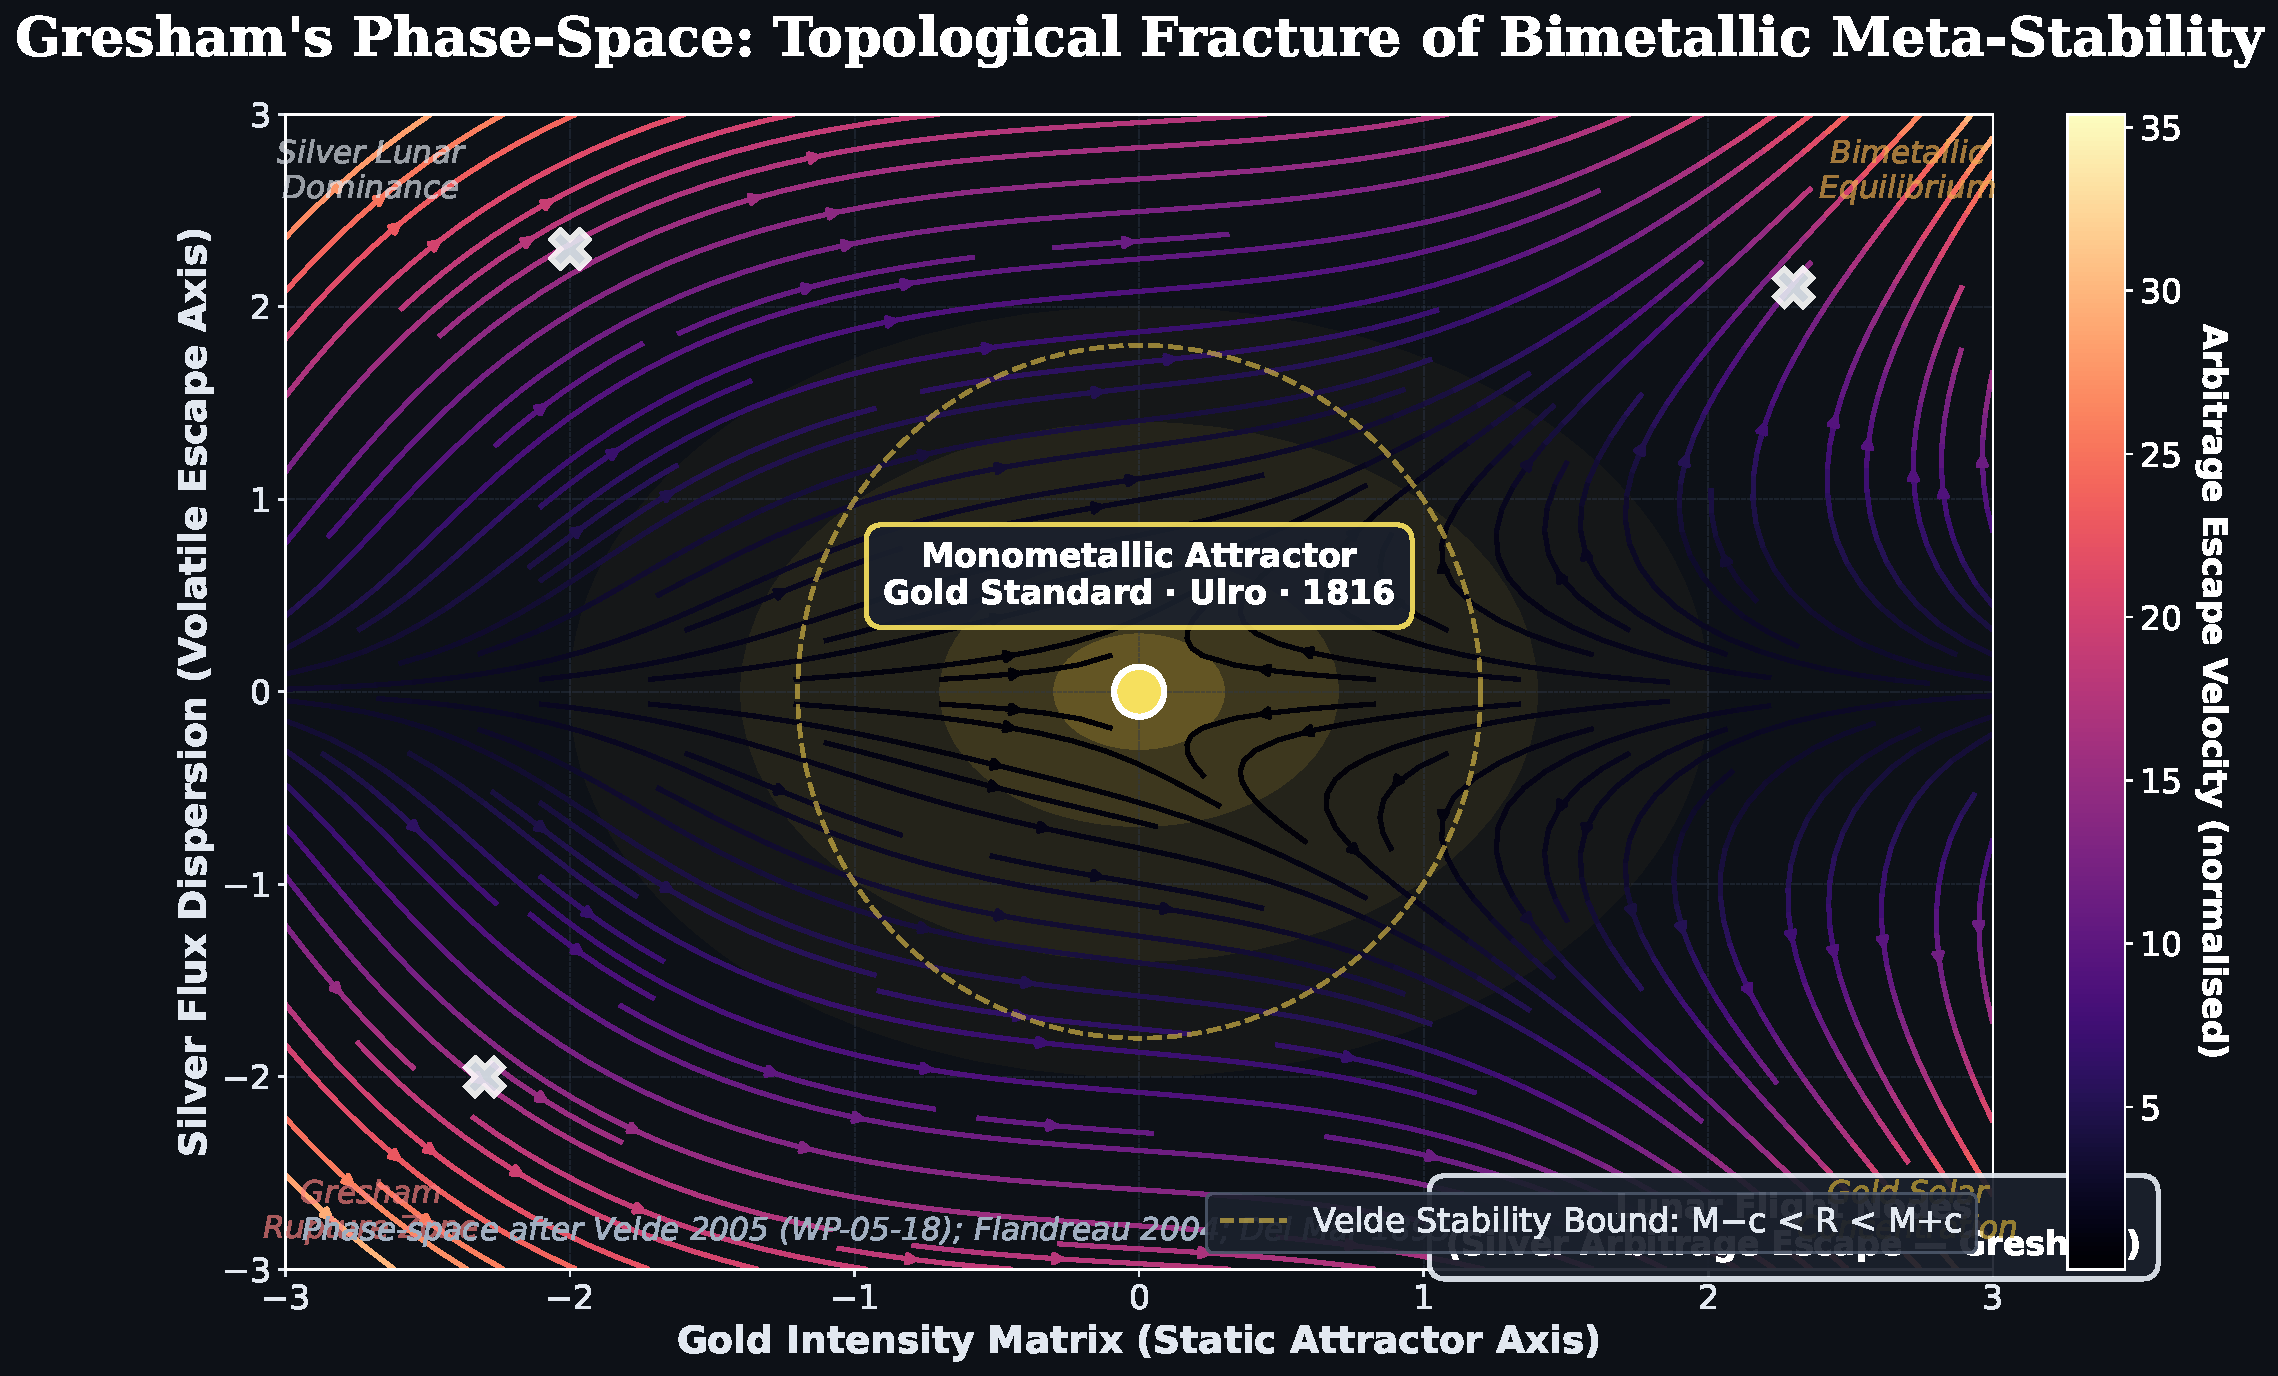
\includegraphics[keepaspectratio,alt={Topological Fracture of Gresham's Law in Phase-Space. This dynamic magma streamplot on a 120×120 grid visualizes the macroeconomic collapse of bimetallic metastability. An overlaid dashed golden ellipse denotes the Velde stability boundary M - c \textless{} R \textless{} M + c. The geometric center (Gold Attractor, m\_S \textbackslash to 0 / Ulro / 1816 Singularity, rendered with a four-layer glow ring) exerts an inflexible inward-pulling vector field (U = -X + 2Y\^{}2)---the gravitational well of the monometallic standard: the 22-carat sovereign at 123.274 grains freezing human exchange into static atoms of sovereign credit. The outward thermal-gradient vectors represent the Lunar Flight (V = 0.5Y + YX\^{}2): silver arbitrage shattering its state-mandated bond into three distinct silver flight nodes (marker `X'). As the Mint Ratio (M) diverges structurally from the international Market Ratio (R), the currency system undergoes topological clinamen out of the bimetallic equilibrium quadrant into the Gresham rupture zone. The 1816 Coinage Act enforced the terminal Urizenic amputation of silver, restricting token coinage to 40 shillings.}]{../figures/topological_fracture_dark.pdf}}
\caption{Topological Fracture of Gresham's Law in Phase-Space. This
dynamic magma streamplot on a 120×120 grid visualizes the macroeconomic
collapse of bimetallic metastability. An overlaid dashed golden ellipse
denotes the Velde stability boundary \(M - c < R < M + c\). The
geometric center (Gold Attractor, \(m_S \to 0\) / Ulro / 1816
Singularity, rendered with a four-layer glow ring) exerts an inflexible
inward-pulling vector field (\(U = -X + 2Y^2\))---the gravitational well
of the monometallic standard: the 22-carat sovereign at 123.274 grains
freezing human exchange into static atoms of sovereign credit. The
outward thermal-gradient vectors represent the Lunar Flight
(\(V = 0.5Y + YX^2\)): silver arbitrage shattering its state-mandated
bond into three distinct silver flight nodes (marker `X'). As the Mint
Ratio (\(M\)) diverges structurally from the international Market Ratio
(\(R\)), the currency system undergoes topological clinamen out of the
bimetallic equilibrium quadrant into the Gresham rupture zone. The 1816
Coinage Act enforced the terminal Urizenic amputation of silver,
restricting token coinage to 40 shillings.}\label{fig-topology}
\end{figure}

\subsection{The Victory of ``Single Vision \& Newton's
Sleep''}\label{the-victory-of-single-vision-newtons-sleep}

This systemic reduction was the ultimate victory of ``Single vision \&
Newtons sleep'' (as Blake declared in his 1802 letter to Butts; Erdman
p.~720) \citep{erdman1988complete}. It represented a reduction of the
regenerate 4-fold man back into an isolated, atomized economic cog,
evaluated solely against the geometric weight of the new golden
sovereign coin. It was a regression into intellectual and spiritual
infancy under the guise of scientific finance, establishing a paradigm
of scarcity that Blake would fight until his last breath. The arc from
Newton's 1717 ratio through the 1797 Restriction to the 1816 Act traces
a complete Blakean narrative: from the imposition of Urizenic geometry
upon the living economy, through the chaotic void of paper abstraction,
to the final re-assertion of monometallic control. Blake's prophetic
response---the immense, unfinished architecture of \emph{Jerusalem},
composed across exactly these years---constitutes the most sustained
imaginative resistance to this economic ontology in the entire literary
canon.

\newpage

\section{Structural Finance History: Blake and Alexander Del Mar
Compared}\label{structural-finance-history-blake-and-alexander-del-mar-compared}

If William Blake provided the visionary, mythopoetic critique of
18th-century monetary metaphysics, the late 19th-century historian
Alexander Del Mar provided its rigorous historiographical counterpart.
Del Mar's \emph{History of Monetary Systems} (1895) operates on a
fundamental thesis that maps onto Blakean cosmology: that the right to
coin money is a sovereign, communal prerogative (a state of Edenic or at
least Beulah-like integration) that has been recurrently hijacked
throughout history by private, atomizing mercantile interests (Urizen)
\citep{delmar1895history}.

\subsection{The Sacred Sovereign Prerogative of Currency and Coinage
Issuance}\label{the-sacred-sovereign-prerogative-of-currency-and-coinage-issuance}

For Del Mar, the structural core of monetary history is precisely this
struggle over the prerogative of issuance. When the state controls the
money supply, value is derived from the \emph{societal totality} (the
Human Form Divine) and the collective needs of the people. When private
banks (such as the Bank of England in 1797) or rigid metallic ratios
(Newton in 1717, Liverpool in 1816) assume control, value is transferred
to the dead material of the coin itself or the fictional ledger of the
private creditor \citep{clapham1944bank}. Rather than asserting
intrinsic metallic value, Del Mar traces the origins of money to
numerary systems maintained by state authority, a thesis that reveals
the transition from bimetallism to the gold standard not merely as a
policy adjustment but as a metaphysical revolution: the displacement of
a communal mechanism by a rigid, materialist reduction. This perspective
illuminates a \emph{generic} economic principle: every monetary regime
encodes a specific theology of value.

\subsection{Blake's Jerusalem Plate 10 and the Architecture of
Enslavement}\label{blakes-jerusalem-plate-10-and-the-architecture-of-enslavement}

Blake recognized this identical usurpation with prophetic clarity. His
condemnation of the Bank of England, the Mint, and the gold standard was
rooted in his understanding that whoever controls the semiotics of value
controls the human soul. On \emph{Jerusalem} Plate 10, Los refuses to
``Reason \& Compare'' on another man's terms and asserts creative agency
as the ground of valuation (\emph{Jerusalem}, lines 20--21; Erdman
p.~153) \citep{erdman1988complete}---the full lines appear in
\hyperref[sec-four-levels-vision]{§ Fourfold Vision}.

That stance is precisely this recognition that the \emph{architecture}
of representation determines the freedom or subjugation of human life.
The ``System'' Blake must create is not merely a mythological schema but
an entire alternative regime of valuation---one grounded in the
irreducible particularity of creative labor rather than the abstract
universality of the gold sovereign. When Del Mar catalogs the social
consequences of the demonetization of silver---how the contraction of
the monetary base enriched the creditor class while plunging the
producing classes into deflationary poverty---he is documenting the
literal effects of Urizen's ``brazen quadrant'' upon the British and
global economy \citep{delmar1885history}.

\subsection{The 1844 Bank Charter Act and Ledger-Driven Spectral
Value}\label{the-1844-bank-charter-act-and-ledger-driven-spectral-value}

The culmination of this architectural subjugation occurred with the 1844
Bank Charter Act (Peel's Act). The fiercely contested debate between the
Banking School and the Currency School narrowed the legal field for note
issue by constraining it under the Bank of England and a statutory
reserve framework with a fixed fiduciary issue. The Currency School
theorists, acting as the ultimate architects of Urizenic geometry,
believed they had finally imprisoned the chaos of economic swerve within
the immutable predictability of the gold standard.

However, by focusing on paper notes, Peel's Act paradoxically ignored
the explosive growth of bank deposits and ledger credit, which later
came to dominate everyday monetary circulation in late 19th-century
Britain. The ``fictive'' or ``spectral value'' against which Blake raged
did not vanish; rather, the ``ghosts'' completely migrated out of the
physical paper artifact and into the invisible, unregulated abstraction
of the bank ledger. This endogenous expansion of invisible credit
represents a profound ontological mutation of the capitalist economy---a
system sustained by mathematical promises that periodically collapsed in
late-century panics.

\subsection{The Convergence of Prophetic and Historiographic Critique:
Del Mar and
Blake}\label{the-convergence-of-prophetic-and-historiographic-critique-del-mar-and-blake}

Both Blake and Del Mar understood that the true ``alchemy'' of money had
been stolen from the domain of human creativity. The living, breathing
economy of human interaction had been replaced by a ledger-bound
numerical simulation engineered to perpetually enrich the creditor class
at the direct expense of the producing masses. Reading Blake through
this historiographic lens elevates his poetic epics from obscure
mystical allegories into profound critiques of modern central banking
and financialized alienation
\citep{poovey2008genres, baucom2005specters}. Del Mar's key
historiographic insight---that the demonetization of silver was a
deliberate political act designed to redistribute wealth upward---finds
its mythopoetic expression in Blake's \emph{Jerusalem}, where the
architects of financial enclosure are exposed as agents of Urizenic
tyranny.

By the \emph{Milton} injunction against counting gold as ultimate good
(see \hyperref[sec-illuminated-nonduality]{§ Illuminated Nonduality})
\citep{erdman1988complete}, Blake stands alongside Del Mar as a prophet
declaring that the highest sovereign act is not the balancing of a
metallic ratio, but the liberation of the human imagination from the
ledger. Where Del Mar provides the forensic historiography, Blake
provides the visionary horizon: together, they articulate a complete
mythopoetic economics of human liberation.

\newpage

\section{The Atlantic Crucible: American Bimetallism and the
Architecture of Republican
Money}\label{the-atlantic-crucible-american-bimetallism-and-the-architecture-of-republican-money}

In 1793---the same year the British state declared war on revolutionary
France and intensified its repression of radical publishers---William
Blake etched \emph{America a Prophecy} on eighteen copper plates in his
Lambeth workshop. Blake was no isolated mystic: David Erdman documents
that he moved through the radical circles of 1790s London, frequenting
the weekly dinners at Joseph Johnson's bookshop in St Paul's Churchyard
alongside Mary Wollstonecraft, William Godwin, and Thomas Paine
\citep{erdman1954prophet}. Erdman further reports that Blake warned
Paine during the government's pursuit of him for seditious libel after
\emph{Rights of Man} (1791--92), helping him avoid arrest and leave for
France (Erdman p.~200). The poem that emerged from this milieu presents
the American Revolution not as a political event but as a cosmic
conflagration: the unchaining of Orc, the spirit of revolutionary
energy, against the tyranny of Urizen's law. But \emph{America a
Prophecy} is not merely a poem about political revolution; it is, when
read alongside the concurrent monetary crises of both Britain and the
newly constituted United States, a prophetic meditation on the
fundamental relationship between monetary sovereignty, human freedom,
and the architecture of value itself. Blake's prophetic structure
anticipates what the American Pragmatists---Peirce, James, Dewey---would
later formalize: the organism confronting a novel encounter, breaking
inherited habit, and forging new modes of engagement with the
indeterminate situation \citep{friedman2026blake, friedman2026doors}.
The American monetary experiment was precisely such an indeterminate
situation, demanding new cognitive and institutional architectures.

\subsection{The Coinage Act of 1792: Hamilton's Republican
Experiment}\label{the-coinage-act-of-1792-hamiltons-republican-experiment}

On 2 April 1792---one year before Blake etched
\emph{America}---President George Washington signed the Coinage Act of
1792, establishing the United States Mint in Philadelphia and codifying
a bimetallic standard with a gold-to-silver ratio of 15:1
\citep{laughlin1898bimetallism}. This ratio, proposed by Treasury
Secretary Alexander Hamilton in his \emph{Report on the Establishment of
a Mint} (1791), was itself an act of deliberate divergence from Newton's
British ratio of 1:15.21 \citep{hamilton1791report}. Hamilton explicitly
calculated his ratio by surveying average European market conditions,
aiming for a standard that would attract both metals into domestic
circulation rather than suffer the asymmetric drainage that plagued
Britain \citep{sylla2018hamiltons}. The silver dollar was defined at
371.25 grains of pure silver; the gold eagle at 247.5 grains of pure
gold. As Richard Sylla and David Cowen demonstrate, Hamilton's financial
architecture---encompassing the Mint, the First Bank, and the systematic
funding of revolutionary war debt---was the most ambitious experiment in
republican finance the modern world had yet attempted
\citep{sylla2018hamiltons}.

This legislative act was revolutionary in its monetary implications, yet
it carried a structural flaw that would destabilize the American economy
for a century. Where Newton's Mint had served the Crown's imperial
prerogative---calibrating a 15.21:1 ratio that systemically overvalued
gold and drained England of silver---Hamilton designed his 15:1 ratio
for a republican experiment in dual-metal equilibrium. However, as
Angela Redish demonstrates in \emph{Bimetallism: An Economic and
Historical Analysis}, Hamilton's flatter ratio sat ``on the slope of a
declining value of silver relative to gold,'' driven by oversupply from
Latin American mines \citep{redish2000bimetallism}. Consequently,
Hamilton inadvertently overvalued silver. This triggered Gresham's Law
in reverse: gold coins were melted and exported to Europe where they
commanded a higher premium, leaving the United States on a \emph{de
facto} silver standard by 1834. As Lawrence Officer calculates, the U.S.
Mint earned substantial seigniorage profit from the operation of the
bimetallic system despite its structural instability, suggesting the
arrangement served fiscal as well as monetary purposes
\citep{officer2001bimetallism}. Milton Friedman and Anna Schwartz later
analyzed this initial miscalibration as guaranteeing the monetary
volatility that would define 19th-century America
\citep{friedman1963monetary}. Curtis Nettels' study of the early
national economy confirms that Hamilton's system, however flawed in its
ratio, succeeded in establishing the institutional architecture---Mint,
Treasury, funded debt---upon which American monetary sovereignty would
depend \citep{nettels1962emergence}.

Blake's Orc, breaking free from his chains on the Atlantean mountains,
embodies precisely this revolutionary energy---the structural analogue
to Peirce's ``irritation of doubt'' that compels genuine inquiry: the
encounter with an indeterminate situation that inherited habit cannot
resolve \citep{friedman2026blake}. The Preludium to \emph{America}
(Plates 1--4) depicts Orc's liberation as an elemental eruption: the
``hairy youth'' bursts his chains in a subterranean cavern, his body
burning with the fire of revolutionary desire (Erdman pp.~51--52)
\citep{erdman1988complete}. When we read this mythological unchaining
alongside the simultaneous establishment of a new monetary sovereign---a
nation explicitly rejecting the Bank of England's monopoly, the Crown's
prerogative of issuance, and the Newtonian metrological regime---Orc's
fire becomes legible as the liberation of value itself from the calculus
of empire.

\subsection{Hamilton vs.~Jefferson: The Structural Antinomy of
Republican
Finance}\label{hamilton-vs.-jefferson-the-structural-antinomy-of-republican-finance}

The American experiment in bimetallism was, from its inception, riven by
an internal antinomy that maps with remarkable precision onto Blake's
mythological framework. Alexander Hamilton---the architect of the First
Bank of the United States (chartered 1791)---envisioned a centralized
financial architecture modeled on, though deliberately constrained
relative to, the Bank of England. Hamilton's bank, capitalized at \$10
million, was authorized to issue banknotes, manage federal debt, and
coordinate fiscal policy---functions that Thomas Jefferson viewed as a
direct assault on republican agrarian virtue
\citep{laughlin1898bimetallism, wilentz2005rise}.

Jefferson's opposition to the Bank was not merely constitutional (though
he argued strenuously that the Constitution granted no power to charter
a federal bank); it was ontological. Jefferson insisted that the
productive labor of the farmer---the physical working of the
earth---constituted the only legitimate foundation of national wealth.
Paper credit, fractional reserve banking, and the abstractions of urban
finance were, in Jefferson's view, parasitical fictions that enriched
speculators at the expense of the producing classes. As Sean Wilentz
documents in \emph{The Rise of American Democracy}, this
Hamilton-Jefferson divide defined the fundamental fault line of American
political economy for the next century, structuring every subsequent
conflict over banking, tariffs, and monetary standards
\citep{wilentz2005rise}. This position resonates with Blake's
\emph{Jerusalem} critique of allegoric riches (see
\hyperref[sec-allegoric-riches]{§ The fixing of labour and allegoric
riches}) \citep{erdman1988complete, sklar2011blake}: both Blake and
Jefferson recognized that the architecture of money creation determined
the distribution of real power and real suffering. Saree Makdisi's
analysis of Blake's impossible history extends this parallel further,
arguing that Blake's rejection of state-administered personhood and
property---the very foundations upon which both Hamiltonian credit and
Jeffersonian land-ownership depend---constitutes a more radical critique
than either political faction could articulate
\citep{makdisi2003william, makdisi2014reading}.

Yet Jefferson's agrarian alternative was itself caught in the
contradictions of commodity production. The Jeffersonian farmer remained
dependent on metallic currency---on the very gold and silver whose
statutory ratios, as Gresham's Law demonstrated, were subject to
international arbitrage beyond any single nation's control. Blake's
prophetic critique extends further than either Hamilton's centralized
finance or Jefferson's agrarian metallist position: for Blake, the
fundamental error is the reduction of value to \emph{any} quantitative
metric, whether gold, silver, or paper. \emph{The Book of Thel} (1789)
refuses that reduction in the terms of coined wisdom and love
\citep{blake1789thel}---see \hyperref[sec-urizenic-materialism]{§
Urizenic materialism}---and the same logic bears on Hamilton's Treasury
notes and Jefferson's silver dollars. Blake's Fourfold Vision---the
coordination of Urizen (reason), Luvah (passion), Tharmas (sensation),
and Urthona (imagination)---constitutes a proto-cognitive architecture
in which no single faculty may dominate without fragmenting the system
into what Blake names ``Newton's Sleep''
\citep{friedman2026blake, friedman2026doors}. The Hamilton-Jefferson
antinomy is, in this reading, a \emph{bifurcation} of the American
political mind: reason (Hamilton) sundered from embodied agricultural
sensation (Jefferson), with neither capable of the integrative Fourfold
Vision that Blake demanded.

\newpage

\section{\texorpdfstring{\emph{America a Prophecy} and the Political
Economy of Revolutionary
Perception}{America a Prophecy and the Political Economy of Revolutionary Perception}}\label{america-a-prophecy-and-the-political-economy-of-revolutionary-perception}

\subsection{``Shaking their mental chains'': Blake's Prophecy at the
Monetary
Threshold}\label{shaking-their-mental-chains-blakes-prophecy-at-the-monetary-threshold}

\emph{America a Prophecy} (1793) is structured in two movements: a
Preludium of mythological unchaining and a Prophecy of revolutionary
confrontation. At its center lies a passage of economic and
epistemological resonance. When the Thirteen Governors convene in
Bernard's house and the flames of Orc engulf the land, the colonial
administrators react with terror:

\begin{quote}
``Shaking their mental chains, they rush in fury to the sea To quench
their anguish; at the feet of Washington down fall'n They grovel on the
sand and writhing lie'' (\emph{America a Prophecy}, Plates 13--14;
Erdman p.~55) \citep{erdman1988complete, blake1793america}
\end{quote}

The phrase ``mental chains'' is Blake's articulation of the relationship
between political subjugation and epistemic imprisonment. These are not
physical manacles but conceptual constraints---the same ``mind-forg'd
manacles'' that Blake would later identify in \emph{London} (Songs of
Experience, 1794; Erdman p.~70) \citep{erdman1988complete}. In the
context of the bimetallic monetary crisis, the ``mental chains'' are the
very statutory ratios, fixed prices, and abstract ledgers that bind
human labor to metallic equivalences. The governors do not merely lose
political authority; they lose the entire conceptual apparatus through
which they have administered value.

An analysis of \emph{America a Prophecy} formalizes this dynamic as
\emph{anticipatory epistemology}: the Thirteen Governors' collapse
enacts the dissolution of a cognitive prior---what Peirce would later
call the dissolution of a ``fixation of belief''---that can no longer
sustain itself against the pressure of experience
\citep{friedman2026blake, friedman2026doors}. The governors' ``mental
chains'' are not merely political ideology but cognitive
priors---inherited models of imperial sovereignty that the American
encounter renders inoperative. When they ``rush in fury to the sea,''
they seek to quench the Orcian fire that has falsified their generative
model, but the old prior cannot be restored. This is Dewey's
``indeterminate situation'' realized in mythic form: the moment when
inherited habits of thought break down and genuine inquiry---or genuine
revolution---becomes unavoidable.

\subsection{Boston's Angel and the Commodification of Trade and
Generosity}\label{bostons-angel-and-the-commodification-of-trade-and-generosity}

The most economically resonant passage in \emph{America} is Boston's
Angel's speech, which Blake positions as the poem's intellectual climax:

\begin{quote}
``Who commanded this? What God? What Angel? To keep the gen'rous from
experience till the ungenerous Are unrestrain'd performers of the
energies of nature; Till pity is become a trade, and generosity a
science That men get rich by; and the sandy desert is giv'n to the
strong?'' (\emph{America a Prophecy}, Plate 9; Erdman p.~53)
\citep{erdman1988complete, blake1793america}
\end{quote}

This passage demands economic exegesis. ``Pity is become a trade''
anticipates by eighty years Karl Marx's analysis of how capitalism
transforms all human relations into commodity relations: even compassion
itself becomes a tradeable asset, a resource to be deployed for profit.
``Generosity a science / That men get rich by'' describes with precision
the logic of speculative philanthropy, charitable endowments, and the
broader financialization of human virtue that was already visible in the
operations of the Bank of England's credit system
\citep{poovey2008genres}. Patrick Brantlinger's \emph{Fictions of State}
traces how this transformation of moral sentiment into financial
infrastructure extended through the entire edifice of 18th-century
credit culture, creating what he terms a ``culture of speculation'' in
which even patriotism and public spirit were securitized
\citep{brantlinger1996fictions}.

Boston's Angel's declaration---``No more I follow, no more obedience
pay!''---is the decisive act of the anticipatory moment: the organism
breaking inherited habit and asserting a new mode of engagement with the
world \citep{friedman2026blake}. The Angel does not merely reject a
particular policy; he rejects the entire epistemological framework
within which imperial monetary administration operates. As Makdisi
argues, Blake's \emph{America} challenges the emerging commodity-form of
perception itself: the idea that knowledge, like goods, is something
passively received from external authority rather than actively produced
through imaginative engagement \citep{makdisi2003william}. Boston's
Angel demands to know \emph{who has the right to restrict
experience}---a question that applies with equal force to the
sovereign's right to fix the price of metal and the Bank's right to
restrict the conversion of paper into gold. Jon Mee's \emph{Dangerous
Enthusiasm} contextualizes Blake within the broader culture of 1790s
radical dissent, demonstrating that Blake's critique of commodified
experience drew directly on the millenarian and antinomian traditions
that informed popular resistance to enclosure, taxation, and the
disciplinary apparatus of Pitt's wartime state \citep{mee1992dangerous}.

\subsection{The ``Crime'' of 1873 and the Demonetization of
Silver}\label{the-crime-of-1873-and-the-demonetization-of-silver}

Blake's prophetic framework proves its relevance when extended beyond
its immediate historical context to encompass the full arc of American
bimetallic politics. The Fourth Coinage Act of 12 February 1873---known
to its critics as ``The Crime of 1873''---demonetized the silver dollar
by omitting it from the list of authorized coins, effectively placing
the United States on a gold monometallic standard
\citep{laughlin1898bimetallism}. This legislative act, passed with
minimal public debate while the nation was still recovering from Civil
War and the Reconstruction crisis, enacted on American soil the same
regression that Blake had diagnosed in Britain's 1816 Coinage Act. As
Richard White documents in \emph{The Republic for Which It Stands}, the
1873 Act was not a sudden conspiracy but the culmination of a
decade-long lobbying campaign by Eastern financial interests who sought
to align American monetary policy with the emerging international gold
consensus centered on London and Berlin \citep{white2017republic}.

The parallels with the British experience are structurally exact. Where
Lord Liverpool's 1816 Act (56 Geo. III c.68) demonetized full-bodied
silver by reducing it to token coinage with a 40-shilling legal tender
limit, the 1873 Act accomplished the same amputation by erasing the
silver dollar from the statute book. As Marc Flandreau argues in
\emph{The Glitter of Gold}, this global shift from bimetallism to gold
was fundamentally a struggle over \emph{political theology}---a contest
between competing visions of what money \emph{is} and whom it should
serve \citep{flandreau2004glitter}. Agrarian producers and Western
miners defended silver as a tangible sacrament of their labor, while
Eastern financial elites demanded the hierarchical, centralized
abstraction of the gold standard. Richard Franklin Bensel's
\emph{Political Economy of American Industrialization} demonstrates that
the deflation following 1873 was not an incidental consequence but a
structural requirement of the gold standard regime, which transferred
wealth systematically from debtor agrarians to creditor financiers
\citep{bensel2000political}.

Where Newton's Mint ratio had overvalued gold to drain England of
silver, the post-1873 deflation crushed American farmers under a
contracting gold supply---what Milton Friedman and Schwartz documented
as a roughly 50\% collapse in American price levels between 1865 and
1896 \citep{friedman1963monetary}. The producing classes of both
nations---the ``laborious'' upon whom Blake's ``Councellor'' throws the
``curb / Of Poverty'' (\emph{Jerusalem}, Plate 27; Erdman p.~170)---bore
the consequences of this monetary contraction, while the urban creditor
class reaped profits from the rising value of their gold-denominated
claims \citep{delmar1895history, erdman1988complete}.

\subsection{The Free Silver Movement and the Populist
Insurgency}\label{the-free-silver-movement-and-the-populist-insurgency}

The political response to the Crime of 1873 constituted nothing less
than the most significant challenge to financial orthodoxy in American
history. The Free Silver movement (1873--1900) demanded the restoration
of free coinage of silver at a ratio of 16:1---a deliberate rejection of
the monometallic stranglehold that had impoverished the agrarian West
and South \citep{laughlin1898bimetallism}. Charles Postel's \emph{The
Populist Vision} demonstrates that the Populists were not, as Richard
Hofstadter once dismissively characterized them, backward-looking
agrarian romantics, but sophisticated political actors who understood
the monetary system's structural biases with considerable analytical
precision \citep{postel2007populist, hofstadter1955age}. Congress
responded with the Bland-Allison Act of 1878, requiring the Treasury to
purchase \$2--4 million of silver bullion monthly for coinage, and the
Sherman Silver Purchase Act of 1890, mandating the purchase of 4.5
million ounces of silver per month---legislative interventions that
represented partial attempts to restore the bimetallic synthesis against
the crushing monometallism imposed by Eastern financial interests.

The movement reached its crescendo in William Jennings Bryan's ``Cross
of Gold'' speech at the 1896 Democratic National Convention in Chicago
(9 July 1896). As Michael Kazin documents in \emph{A Godly Hero},
Bryan's address was not merely a political performance but a
distillation of two decades of agrarian frustration with the
deflationary gold standard regime \citep{kazin2006godly}. His defense of
the agrarian producing classes against urban financial elites
recapitulates with precision Blake's insistence that productive,
embodied labor constitutes the only true source of value
\citep{laughlin1898bimetallism}. Bryan even invoked the American
Revolution explicitly: ``instead of having a gold standard because
England has, we shall restore bimetallism, and then let England have
bimetallism because the United States have''---a deliberate re-enactment
of 1776's monetary independence. This is the Orcian fire, transmitted
across a century: the same demand for liberation from the imperial
metric that Blake had inscribed in \emph{America a Prophecy}.

Bryan's peroration constitutes one of the most powerful expressions of
the critique of monometallism ever uttered in the American political
tradition:

\begin{quote}
``Having behind us the producing masses of this nation and the world,
supported by the commercial interests, the laboring interests, and the
toilers everywhere, we will answer their demand for a gold standard by
saying to them: `You shall not press down upon the brow of labor this
crown of thorns; you shall not crucify mankind upon a cross of
gold.'\,''
\end{quote}

The image of crucifixion upon gold directly inverts the Christian
symbolism that Blake deployed throughout his prophetic works: gold,
which should represent the solar principle of divine love, has been
weaponized into an instrument of torture---the miser's guinea elevated
above the sun until it becomes the cross upon which human labor is
sacrificed. Bryan's speech echoes Blake's \emph{Milton} refusal to treat
bullion as the highest good (see \hyperref[sec-illuminated-nonduality]{§
Illuminated Nonduality}) \citep{erdman1988complete}. Yet Bryan lost the
1896 election to William McKinley---the candidate of gold and industrial
capital---and the Gold Standard Act of 1900 formally enthroned the
monometallic regime, ending the American bimetallic experiment that
Hamilton had initiated 108 years earlier. The Urizenic prior,
momentarily destabilized by Orc's populist fire, reconsolidated itself
in institutional form---precisely as \emph{America a Prophecy} predicts:
Urizen descends again, his ``icy magazine'' poured upon the
revolutionary flames.

\newpage

\section{Transatlantic Architectures of Monetary Collapse: Britain and
America
Compared}\label{transatlantic-architectures-of-monetary-collapse-britain-and-america-compared}

\subsection{The Divergent Ratios and Their Structural
Consequences}\label{the-divergent-ratios-and-their-structural-consequences}

The British and American bimetallic experiments, though sharing the same
architecture---two metals bound by statutory fiat---diverged in ways
that illuminate both the generic logic of bimetallic instability and the
specific political economies encoded in each nation's monetary regime. A
systematic comparison reveals how Gresham's Law operated with identical
structural logic but divergent political consequences across the
Atlantic.

{\def\LTcaptype{none} % do not increment counter
\begin{longtable}[]{@{}
  >{\raggedright\arraybackslash}p{(\linewidth - 4\tabcolsep) * \real{0.2037}}
  >{\raggedright\arraybackslash}p{(\linewidth - 4\tabcolsep) * \real{0.3704}}
  >{\raggedright\arraybackslash}p{(\linewidth - 4\tabcolsep) * \real{0.4259}}@{}}
\toprule\noalign{}
\begin{minipage}[b]{\linewidth}\raggedright
Parameter
\end{minipage} & \begin{minipage}[b]{\linewidth}\raggedright
Britain (1717--1816)
\end{minipage} & \begin{minipage}[b]{\linewidth}\raggedright
United States (1792--1873)
\end{minipage} \\
\midrule\noalign{}
\endhead
\bottomrule\noalign{}
\endlastfoot
Statutory Ratio & 1:15.21 (Newton, 1717) & 1:15 (Hamilton, 1792);
revised to 1:16 (1834) \\
Market Reality & \textasciitilde1:14.5 (European) &
\textasciitilde1:15.5 (European, post-1792) \\
Direction of Drainage & Silver exported to France/India & Gold exported
to Europe (pre-1834); Silver exported (post-1834) \\
Central Bank & Bank of England (1694) & First Bank of US (1791--1811);
Second Bank (1816--1836) \\
Suspension Event & Privy Council order, 26 Feb 1797; Royal Assent, 3 May
1797 & Suspension of specie convertibility, 1862--1879 \\
Demonetization & Coinage Act 1816 (56 Geo. III c.68) & Fourth Coinage
Act, 12 Feb 1873 \\
Popular Resistance & Minimal (no Free Silver equivalent) & Free Silver
movement (1873--1900) \\
Prophetic Critique & Blake's \emph{Jerusalem}, \emph{Milton} & Bryan's
``Cross of Gold'' (1896) \\
\end{longtable}
}

The table reveals a structural insight: under Hamilton's 15:1 ratio,
which \emph{undervalued} gold relative to the European market of
approximately 15.5:1, the United States initially experienced the mirror
image of Britain's drainage. American gold was exported to Europe where
it commanded higher value, while silver accumulated
domestically---making silver, paradoxically, the \emph{de facto}
American standard through the 1820s
\citep{laughlin1898bimetallism, officer2001bimetallism}. This is
precisely the inverse of Britain's experience under Newton's 15.21:1
ratio, which overvalued gold and drained silver. The 1834 revision to
approximately 16:1 reversed this dynamic, deliberately overvaluing gold
to attract it into domestic circulation---but at the cost of triggering
the same outward silver flight that had devastated British coinage a
century earlier \citep{redish1990evolution}.

\subsection{Jackson's War on the Bank: The Limits of Institutional
Destruction}\label{jacksons-war-on-the-bank-the-limits-of-institutional-destruction}

Andrew Jackson's veto of the Second Bank of the United States in 1832,
followed by his executive removal of federal deposits in 1833 and the
Bank's ultimate demise in 1836, constitute an episode of resonance for
understanding the structural limits of monetary reform. Jackson, the
agrarian populist from the frontier, declared the Bank a ``monopoly''
and a ``hydra of corruption'' that enriched Eastern financial elites at
the expense of the producing classes
\citep{howe2007what, wilentz2005rise}. Daniel Walker Howe's \emph{What
Hath God Wrought} demonstrates that Jackson's Bank War was not merely an
economic dispute but a fundamental contest over the meaning of
democratic sovereignty in the new republic: who should control the
creation of money, and to whose benefit \citep{howe2007what}?

In Blake's mythological terms, this is Orc's revolutionary assault on
the Urizenic institution---the fiery destruction of the centralized
architecture of credit. Yet Jackson's destruction of the Bank unleashed
a ``Free Banking'' era of wildcat state-chartered institutions that
issued unregulated paper currency---precisely the proliferating
``allegoric riches'' Blake treats in \hyperref[sec-allegoric-riches]{§
The fixing of labour and allegoric riches}, now scaled horizontally
across state charters. Sean Wilentz documents how the period between the
Bank's destruction (1836) and the Civil War saw over 1,600
state-chartered banks issuing their own notes, producing a fragmented,
unreliable, and frequently fraudulent currency system
\citep{wilentz2005rise}.

The Jacksonian paradox recapitulates the Blakean diagnosis with
fidelity: destroying the centralized institution does not automatically
produce liberation. In the language of \emph{America a Prophecy}, where
Orc's revolutionary fire has consumed the old order, Urizen descends
again---reconstituting himself in new institutional forms. This cycle of
revolution and reconsolidation is not a failure of the revolutionary
impulse but a consequence of insufficient cognitive transformation---a
structural feature of Blake's prophetic epistemology
\citep{friedman2026blake, friedman2026doors}. Without the integrative
Fourfold Vision that coordinates all four Zoas---reason, passion,
sensation, and imagination---the destruction of one Urizenic institution
merely clears the ground for another. As Blake writes in \emph{America a
Prophecy}:

\begin{quote}
``Urizen, who sat / Above all heavens, in thunders wrapp'd, emerg'd his
leprous head From out his holy shrine, his tears in deluge piteous
Falling into the deep sublime'' (\emph{America a Prophecy}, Plates
16--17; Erdman pp.~57--58) \citep{erdman1988complete, blake1793america}
\end{quote}

Revolution alone is insufficient; the Urizenic principle merely
reconstitutes itself in new institutional forms. Jackson dismantled the
\emph{federal} monopoly on credit only to democratize the issuance of
unbacked paper through state banks---a horizontal proliferation of the
same abstracting technology. Without the qualitative vision that
transcends both metallic fetishism and paper abstraction, the
destruction of one tyranny merely inaugurates another.

\subsection{The Greenback Suspension: America's Unprecedented Wartime
Monetary
Swerve}\label{the-greenback-suspension-americas-unprecedented-wartime-monetary-swerve}

The American Civil War (1861--1865) produced its own swerve into fiat
abstraction, paralleling the British Bank Restriction of 1797. In 1862,
the United States Treasury began issuing Legal Tender Notes
(``Greenbacks'')---unbacked paper currency designed to finance the Union
war effort. Like the Bank Restriction, the American suspension of specie
convertibility severed the connection between the circulating medium and
any metallic anchor, plunging the economy into a void of fiat
abstraction that persisted until the Specie Resumption Act of 1875
restored gold convertibility on 1 January 1879
\citep{laughlin1898bimetallism, unger1964greenback}.

Irwin Unger's Pulitzer Prize-winning \emph{The Greenback Era}
demonstrates that the suspension was far more than a wartime expedient:
it catalyzed a reorganization of American political coalitions around
the question of what money \emph{is} \citep{unger1964greenback}. The
``soft money'' faction---farmers, debtors, Western
entrepreneurs---demanded the permanent retention of Greenbacks as an
inflationary counterweight to the deflationary gold standard. The ``hard
money'' faction---Eastern bankers, creditors, industrial
capitalists---insisted on resumption and gold convertibility. This
division prefigured and structurally anticipated the Free Silver
movement of the 1880s--1890s.

The structural parallel with Britain is precise: both the 1797 British
suspension and the 1862 American suspension were triggered by
existential military crises; both produced inflationary spirals that
devastated the laboring classes while enriching financial speculators;
and both were resolved by a return to metallic standards that imposed
deflationary austerity upon the producing classes. In both cases,
Blake's prophetic analysis holds: the oscillation between the crushing
geometry of metallic standards and fiat paper constitutes a double
bind---a pendulum swing between two modes of quantification, neither of
which addresses the fundamental crisis of human value.

\subsection{From Albion to America: Prophetic and Monetary
Transmission}\label{from-albion-to-america-prophetic-and-monetary-transmission}

Blake's \emph{America a Prophecy} concludes not with Orc's triumph but
with Urizen's renewed assault---his ``icy magazine'' poured upon the
Atlantic to contain the revolutionary fire for ``twelve years'' before
``France receiv'd the Demon's light'' (Plates 16--17; Erdman pp.~57--58)
\citep{erdman1988complete, blake1793america}. This prophetic
temporality---revolution contained but not extinguished, revolutionary
energy transmitted across borders---maps with precision onto the
transmission of bimetallic crises across the Atlantic. Britain's 1816
demonetization of silver preceded, and structurally anticipated,
America's 1873 demonetization. Barry Eichengreen's \emph{Globalizing
Capital} traces this convergence as part of a broader ``network effect''
in which the gold standard spread not through inherent superiority but
through the gravitational pull of London's capital markets, which made
gold convertibility the price of access to international credit
\citep{eichengreen2019globalizing}.

This transatlantic transmission functions as a key instance of what
Peirce calls the ``community of inquirers''---the recognition that no
single nation's monetary experiment operates in isolation, but that all
are bound in a web of mutual inference and structural feedback
\citep{friedman2026blake}. Blake's prophetic vision anticipated this
insight: Orc's fire cannot be confined to a single continent, and
Urizen's counterrevolution is likewise global. The arc from Newton's
1717 ratio through Hamilton's 1792 ratio, through both nations'
suspensions and ultimate demonetizations of silver, traces a single
structural trajectory: the global establishment of monometallic
quantification over bimetallic generation. Yet the 19th-century gold
standard was merely a transitional phase toward a more radical monetary
abstraction.

\newpage

\section{Consolidating Fiat Abstraction: Federal Reserve to the Nixon
Shock}\label{consolidating-fiat-abstraction-federal-reserve-to-the-nixon-shock}

The arc from Newton's 1717 ratio through Hamilton's 1792 ratio traces a
single structural trajectory: the global establishment of monometallic
quantification over bimetallic generation. Yet the 19th-century gold
standard was merely a transitional phase toward a more radical
abstraction. The defining monetary events of the 20th century---the
establishment of the Federal Reserve (1913), the confiscation of private
gold (1933), the demonetization of silver coinage (1965), and the
collapse of the Bretton Woods system (1971)---constitute the realization
of Blake's \emph{Ulro}: the descent into a fiat void where money is
severed entirely from physical substance.

\subsection{The 1913 Federal Reserve Act: Centralizing the Architecture
of
Issuance}\label{the-1913-federal-reserve-act-centralizing-the-architecture-of-issuance}

On 23 December 1913, Congress passed the Federal Reserve Act, altering
the architecture of American monetary sovereignty by transferring the
power of currency issuance to a centralized, quasi-public banking system
comprising twelve regional Reserve Banks coordinated by the Federal
Reserve Board in Washington, D.C. As William Silber documents in
\emph{When Washington Shut Down Wall Street}, the establishment of the
Federal Reserve was catalyzed not merely by the Panic of 1907 but by a
structural crisis: the absence of a ``lender of last resort'' capable of
providing elastic currency during financial panics---a function the Bank
of England had performed since 1694 \citep{silber2007when}. The Federal
Reserve thus represented the belated American adoption of the
institutional architecture that Blake had identified as the engine of
abstract credit creation.

In Blake's mythological system, the Federal Reserve Act represents the
institutional triumph of the ``Councellor'' who invents, through a kind
of fiat, ``allegoric riches'' (\emph{Jerusalem} 27; see
\hyperref[sec-allegoric-riches]{§ The fixing of labour and allegoric
riches}) \citep{erdman1988complete}. By establishing an elastic currency
supply managed through open market operations and fractional reserve
banking, the Federal Reserve decoupled the dollar from any fixed
metallic constraint, allowing the money supply to expand and contract at
the discretion of an appointed technocratic elite. Liaquat Ahamed's
\emph{Lords of Finance} demonstrates how the central bankers of the
interwar period---Benjamin Strong of the New York Fed, Montagu Norman of
the Bank of England, Émile Moreau of the Banque de France, and Hjalmar
Schacht of the Reichsbank---wielded this discretionary power with severe
economic consequences, their collective mismanagement of the gold
exchange standard directly precipitating the Great Depression
\citep{ahamed2009lords}.

A reading of Blake's Four Zoas as a ``proto-cognitive architecture''
illuminates the Federal Reserve's structural error: the consolidation of
monetary authority in a single faculty---Urizen's reason---detached from
the embodied, sensory, and imaginative dimensions that the other Zoas
represent \citep{friedman2026blake}. The Fed's founding premise---that
rational technocratic management can optimize the money supply---is
precisely the Urizenic fantasy that Blake diagnosed. It operationalizes
``Newton's sleep,'' which functions formally as the pathology of rigid
priors crushing sensory evidence: the belief that a single geometric
framework, administered by a priestly elite, can govern the infinitely
complex organism of economic life \citep{friedman2026doors}. Where the
earlier bimetallic tension decomposed value into two competing metrics,
the fiat regime represents an even deeper loss of structural integrity.
Synergetic wholeness is destroyed when value becomes an arbitrarily
manipulable abstract symbol, severing any remaining anchoring to
physical reality and allowing limitless numerical expansion without
commensurate productive generation.

\subsection{Executive Order 6102: The Confiscation of the Solar
Principle}\label{executive-order-6102-the-confiscation-of-the-solar-principle}

If the Federal Reserve Act abstracted the issuance of money, the onset
of the Great Depression catalyzed the confiscation of the metallic
anchor itself. Under Executive Order 6102 (5 April 1933) and the
subsequent Gold Reserve Act of 30 January 1934, President Franklin D.
Roosevelt mandated the surrender of all privately held gold coins,
bullion, and gold certificates to the Federal Reserve
\citep{roosevelt1933executive}. Private gold ownership was
criminalized---punishable by up to ten years' imprisonment and a
\$10,000 fine---and the metal was collected and revalued from \$20.67 to
\$35.00 per ounce. This 69\% devaluation effectively expropriated the
savings of every American who had held wealth in the constitutionally
mandated medium of exchange, while simultaneously concentrating the
nation's gold in federal vaults at Fort Knox (constructed 1936) and West
Point.

The ``mental chains'' described in \emph{America a Prophecy} had thus
materialized into statutory edicts: the citizen could no longer hold the
physical substance of value. By capturing the gold, the federal
government removed a physical boundary against fiat expansion. The
contemporaneous Silver Purchase Act of 1934, championed by the Western
silver bloc in Congress, attempted to inflate the currency by
nationalizing vast silver reserves and mandating Treasury purchases at
artificially elevated prices. This dual confiscation demonstrates that
the state recognized the necessity of capturing \emph{both} poles of the
bimetallic spectrum to enforce systemic compliance---an institutional
consolidation that Blake's prophetic framework renders legible as the
final enclosure of metallic reality within the Urizenic ledger.

\subsection{The 1965 Coinage Act and the Purging of Circulating
Silver}\label{the-1965-coinage-act-and-the-purging-of-circulating-silver}

This trajectory reached its domestic culmination with the Coinage Act of
23 July 1965, signed by President Lyndon B. Johnson. Driven by acute
shortages resulting from the growing divergence between silver's
commodity value and its face value in coinage---a textbook Gresham's Law
phenomenon in which the metal's intrinsic worth exceeded its nominal
denomination---the Act removed 90\% silver content from circulating
dimes and quarters, replacing them with copper-nickel clad tokens
\citep{johnson1965coinage}. Half dollars were reduced from 90\% to 40\%
silver, and would lose their remaining silver content entirely in 1971.
Johnson acknowledged the magnitude of this transformation in his signing
remarks, assuring Congress that the Treasury's silver reserves would
``keep the price of silver in line with its value in our present silver
coin.''

The purging of silver from everyday exchange completed a process that
had begun with the Crime of 1873. What circulated was no longer physical
wealth but symbolic tokens, dependent entirely on the credibility of the
issuing authority. The United States had achieved domestically what
Blake diagnosed as the terminal condition of Ulro: the total replacement
of intrinsic material substance with abstract, administered fiat.

\subsection{The Nixon Shock and the Global Triumph of Pure
Abstraction}\label{the-nixon-shock-and-the-global-triumph-of-pure-abstraction}

The ontological transformation of money was achieved globally on 15
August 1971, when President Richard Nixon unilaterally terminated the
direct international convertibility of the US dollar to gold.
Confronting the depletion of US gold reserves from a postwar peak of
approximately 20,000 tonnes to roughly 8,133 tonnes, alongside the
deficit financing of the Vietnam War and Great Society programs, Nixon
suspended the gold window that had anchored the post-war Bretton Woods
system since 1944 \citep{steil2013battle, eichengreen2019globalizing}.

Benn Steil's \emph{The Battle of Bretton Woods} documents how Keynes and
White had designed the original system as a managed gold exchange
standard precisely to avoid the deflationary rigidity of the classical
gold standard while preserving some metallic discipline against
inflationary excess \citep{steil2013battle}. Nixon's unilateral
abrogation of this architecture---announced on a Sunday evening without
consulting allied governments---severed the final tether between the
global monetary system and physical reality. The world was plunged into
a purely fiat regime---a system where all global currencies float
against one another, sustained entirely by the credibility, military
power, and institutional inertia of sovereign issuers. As Barry
Eichengreen demonstrates in \emph{Globalizing Capital}, no historical
precedent existed for a global fiat system of this scale; every previous
experiment with unbacked paper money, from the Chinese \emph{jiaozi} of
the Song Dynasty to the French \emph{assignats} of the 1790s, had ended
in inflationary collapse \citep{eichengreen2019globalizing}.

Official US Treasury--owned monetary gold is often reported near 8,133
tonnes (post--Bretton Woods levels; exact totals move with coining and
transfers). Site figures for Fort Knox, West Point, Denver, and related
facilities are components of that sovereign stock, not separate pools to
be summed into a larger national total. Metal vaulted at the Federal
Reserve Bank of New York is predominantly foreign and other custodial
holdings---not US official reserves---so it must not be added to
Treasury aggregates. That accounting split between sovereign stock and
Manhattan custody mirrors the ontological crisis Blake diagnosed: the
ledger's line items and the underlying metal are easy to conflate.
Treasury gold remains officially valued on the books at the statutory
price of \$42.22 per ounce established in 1973, vastly understating
contemporary market reality. Policy discussion since 2025 has examined
historical precedents for sovereign gold revaluations, estimating that
marking US reserves to market would yield proceeds equivalent to roughly
3\% of GDP---a figure that has prompted Congressional interest in
revaluation as a mechanism for sovereign balance sheet management. The
Urizenic ledger maintains its geometric fiction---\$42.22---while the
physical metal trades at a far higher market price.

\newpage

\section{The Sound Money Rebellion: Re-Monetizing Tangible Sovereignty
(1985--2026)}\label{the-sound-money-rebellion-re-monetizing-tangible-sovereignty-19852026}

Yet the resistance to fiat abstraction has proven structurally
persistent. Despite the closure of the gold window in 1971, the demand
for tangible, unmediated value has periodically erupted with
force---most dramatically in the Hunt brothers' attempted silver
accumulation (1979--80) and the subsequent establishment of the American
Gold Eagle (1985) and American Silver Eagle (1986) bullion programs,
which reintroduced sovereign metallic bullion not for circulation but as
constitutionally significant repositories of stored value. By January
2026, the gold-to-silver ratio had compressed from the historical range
of 80--90:1 that prevailed through most of the 2010s toward
approximately 46:1, suggesting a structural reassertion of silver's
monetary premium alongside its growing industrial demand profile.

\subsection{The Legislative Renaissance of American State Monetary
Federalism}\label{the-legislative-renaissance-of-american-state-monetary-federalism}

The battle between ``allegoric riches'' and metallic tangibility has
escalated directly into the 21st century as an assertion of
constitutional sovereignty. Beginning with the \textbf{Utah Legal Tender
Act} (HB 317, signed 25 March 2011), a coalition of US states has
embarked on a coordinated legislative campaign to formally challenge
federal monetary hegemony
\citep{utah2011legal, greene2015understanding}. This movement asserts
that constituent states possess the constitutional authority under
\textbf{Article I, Section 10} of the US Constitution---which
specifically commands that no state shall ``make any Thing but gold and
silver Coin a Tender in Payment of Debts''---to erect a parallel
monetary ecosystem protecting intra-state commerce from the depreciating
trajectory of the fiat dollar.

This constitutional clause is not a footnote; it is the enduring
legislative trace of a vision Blake would have recognized. The Framers
of the 1787 Constitution---working two years before Blake etched
\emph{The Book of Thel} with its metallic interrogative---inscribed into
the supreme law of the republic a mandate that state-level money must be
physically grounded. Article I, Section 10 compels a monetary realism
that the subsequent history of fiat abstraction has sought to render
operationally moot without legally repealing. The contemporary sound
money movement is, in this constitutional reading, not an innovation but
a \emph{re-activation} of dormant foundational law---what Blake's Los,
insisting on the tangible and the particular against the geometric
abstraction of the ledger, would recognize as the reassertion of the
Forge against the Mint.

Between 2011 and 2026, this movement has accelerated with legislative
momentum. As of March 2026, \textbf{at least ten states} have passed
legislation formally operationalizing this constitutional clause:

{\def\LTcaptype{none} % do not increment counter
\begin{longtable}[]{@{}
  >{\raggedright\arraybackslash}p{(\linewidth - 6\tabcolsep) * \real{0.1750}}
  >{\raggedright\arraybackslash}p{(\linewidth - 6\tabcolsep) * \real{0.2750}}
  >{\raggedright\arraybackslash}p{(\linewidth - 6\tabcolsep) * \real{0.1500}}
  >{\raggedright\arraybackslash}p{(\linewidth - 6\tabcolsep) * \real{0.4000}}@{}}
\toprule\noalign{}
\begin{minipage}[b]{\linewidth}\raggedright
State
\end{minipage} & \begin{minipage}[b]{\linewidth}\raggedright
Legislation
\end{minipage} & \begin{minipage}[b]{\linewidth}\raggedright
Year
\end{minipage} & \begin{minipage}[b]{\linewidth}\raggedright
Key Provisions
\end{minipage} \\
\midrule\noalign{}
\endhead
\bottomrule\noalign{}
\endlastfoot
State & Legislation & Year & Key Provisions \\
------- & ----------- & ------ & ---------------- \\
Utah & HB 317 & 2011 & First state to recognize US-minted gold/silver
coins as legal tender \citep{utah2011legal} \\
Oklahoma & SB 862 & 2014 & Legal tender for US-minted coins; full tax
exemption \\
Arizona & HB 2014 & 2017 & Sales tax and capital gains tax exemption on
precious metals \\
Louisiana & HB 396 / SB 232 & 2017/2024 & Sales tax exemption;
reaffirmed legal tender for US coins \\
Wyoming & HB 103 & 2018 & Legal tender recognition; sales tax exempt
\citep{wyoming2018legaltender} \\
Arkansas & Act 595 & 2023 & Full legal tender recognition and tax
exemption \citep{arkansas2023legaltender} \\
Florida & CS/HB 999 & 2025 & Legal tender for payment of debts;
effective July 1, 2026 \citep{florida2025legaltender} \\
Texas & HB 1056 & 2025 & Signed by Governor Abbott June 2025; partial
effect Sept 2026 \citep{texas2025legaltender} \\
Alabama & SB 130 & 2025 & Passed House 102-0; comprehensive legal tender
and tax provisions \citep{alabama2025legaltender} \\
Nebraska & LB 1317 & 2024 & Removes capital gains tax; explicitly
excludes CBDCs from definition of money \citep{nebraska2024metals} \\
\end{longtable}
}

This is not fringe activism. The legislative margins---Alabama's SB 130
passing the House 102-0---indicate broad bipartisan consensus that the
constitutional prerogative of metallic money has been temporarily
suspended rather than lawfully repealed. The Sound Money Defense League
reports broad state-level movement toward reduced taxation on precious
metals, representing a national trend toward the formal re-recognition
of gold and silver's constitutional monetary status.

\subsection{Dismantling the Punitive Tax Architecture of Fiat
Enforcement}\label{dismantling-the-punitive-tax-architecture-of-fiat-enforcement}

A critical dimension of this monetary federalism involves the systematic
dismantling of the tax architecture designed to penalize precious metal
ownership. Under federal tax law, the IRS classifies bullion as a
``collectible'' subject to a 28\% capital gains rate---significantly
higher than the 15--20\% rate applied to stocks, bonds, and real
estate---structurally discouraging its use as a savings vehicle or
transactional medium. This classification uses the tax code to enforce
fiat monopoly: any citizen who seeks to preserve purchasing power in
constitutional money is penalized relative to those who hold Federal
Reserve Notes.

The state-level response has been to systematically strip away these
penalties. Utah's pioneering HB 317 (2011), later joined by additional
measures expanding legal-tender recognition and payment infrastructure,
has been followed by Arizona and Oklahoma's complete exemption of sales
taxes and capital gains on gold and silver; Nebraska's elimination of
state capital gains taxes on metals; and Florida and Alabama's abolition
of sales taxes on bullion acquisitions
\citep{utah2011legal, florida2025legaltender, alabama2025legaltender, nebraska2024metals}.
Nebraska's LB 1317 is particularly significant: in addition to removing
capital gains taxes on precious metals, it explicitly \textbf{excludes
Central Bank Digital Currencies (CBDCs) from the legal definition of
money}---a direct legislative assertion that digital fiat tokens issued
by the Federal Reserve do not constitute constitutionally valid money
\citep{nebraska2024metals}.

By eliminating the tax friction designed to penalize the holding of
physical metal, these states directly challenge the Federal Reserve's
capacity to define and administer the medium of exchange. In the
language of \emph{America a Prophecy}, this is the Thirteen Angels'
collective transformation writ legislative: the states, like Blake's
revolutionary governors who rend their robes and stand with Washington
in the Orcian flames, are breaking with the received institutional
framework---enacting the pragmatist moment of genuine inquiry, where
inherited habit is abandoned in favor of a new mode of engagement with
the indeterminate monetary situation \citep{friedman2026blake}. The
movement explicitly positions itself as a defense of the producing
classes---an insistence that constitutional metals, constrained by
physical scarcity, preserve the purchasing power of labor against the
indefinite expansion of fiat currency. It is the modern institutional
manifestation of Bryan's agrarian crusade, transposed from the prairie
to the statehouse and equipped with precise statutory instruments.

\subsection{The Texas Bullion Depository: Sovereign Infrastructure
Beyond Federal
Custody}\label{the-texas-bullion-depository-sovereign-infrastructure-beyond-federal-custody}

A key structural innovation of this 21st-century resistance is the
establishment of state bullion depositories. In 2015, the Texas
legislature passed \textbf{SB 2097}, creating the \textbf{Texas Bullion
Depository}---launched operationally in 2018 as the first sovereign
institutional infrastructure designed specifically for holding precious
metals reserves outside of the federal banking apparatus
\citep{texas2015depository}. The Depository provides a secure,
state-managed, publicly auditable alternative to the federal
depositories (Fort Knox has not been independently audited since 1953),
and is authorized to accept deposits from individuals, businesses, and
government entities. Governor Abbott's subsequent signing of \textbf{HB
1056} (June 2025) integrates the Depository's infrastructure with the
state's new legal tender framework, creating a vertically integrated
system: Texas citizens can hold gold and silver as legal tender, store
it in a state-managed depository, and transact with it free of state
taxation \citep{texas2025legaltender}.

This infrastructure physically relocates monetary reserves from
centralized Federal Reserve custody into explicitly decentralized,
state-controlled institutions. When mapped onto Blake's prophetic
architecture, this localized legislative reassertion represents the
persistence of what Blake called the productive, creative impulse of
Los---the blacksmith who works with fire and metal at the forge,
insisting on the tangible and the particular against the geometric
abstraction of the ledger. The constitutional text that these states
invoke---Article I, Section 10---was drafted in 1787, two years before
\emph{The Book of Thel} (1789) \citep{blake1789thel}. Over two centuries
later, the tension between abstract ledger and tangible metal endures,
and the legislative campaign to reclaim physical monetary sovereignty
remains a persistent, structural defense of tangible value against the
empire of abstract debt \citep{erdman1988complete}.

\newpage

\section{The Spectral Made Tangible: Precious Metals versus Digital
Abstraction}\label{sec-spectral-2020-2026}

By the third decade of the twenty-first century, the long trajectory
that Blake's prophetic system diagnosed---from bimetallic generation
through monometallic enclosure to pure fiat abstraction---had reached a
critical inflection. The very instruments designed to enforce
ontological groundlessness were generating, through their excess, an
equal and opposite assertion of metallic tangibility. The years 2020 to
2026 constitute the most significant period of precious metal
reassertion since Nixon's closure of the gold window in 1971, driven not
by nostalgia but by recurrent stress in fiat regimes. Read through a
Blakean lens, these years trace the arc from Orc's renewed stirring
beneath the surface to the first coherent legislative and institutional
form of Los's counter-forge, with the gold-to-silver ratio compressing
from a historic peak near 127:1 toward approximately 50:1 by early 2026.

\subsection{The COVID Clinamen and the Pandemic Monetary
Swerve}\label{the-covid-clinamen-and-the-pandemic-monetary-swerve}

The first shock came with precise mythological timing. On 11 March 2020,
the World Health Organization declared COVID-19 a global pandemic.
Within two weeks, the gold-to-silver ratio surged to an extraordinary
\textasciitilde127:1 on 18 March---the highest level in recorded
history---as financial markets liquidated silver alongside industrial
assets, while simultaneously bidding gold toward historic valuations as
a safe-haven instrument. This ratio inversion crystallized the dualism
Blake's bimetallic framework encodes: silver, the lunar metal of
industrial circulation and commercial exchange, collapsed as economic
activity froze globally; gold, the solar metal of pure sovereignty, was
elevated precisely because the sovereign fiat system appeared threatened
\citep{silverinstitute2021world}.

The Federal Reserve's emergency response---expanding its balance sheet
from approximately \$4.2 trillion to over \$7 trillion in four months,
the most aggressive activation of the electronic printing press in
monetary history---constituted a \emph{fiat clinamen}: the swerve into
maximum abstraction. This produced its precise Blakean counter-reaction:
a flight toward the physical, the scarce, the irreducibly material.
Gold, which cannot be printed or conjured from a spreadsheet, reasserted
itself as the terminal hedge against the limitlessness of the ledger
\citep{steil2013battle}.

For Blake, this dynamic is precisely the shape of prophetic crisis---the
point at which Urizen's overextension of geometric abstraction provokes
Orc's eruption. The pandemic monetary swerve confirmed, in real time,
what \emph{America a Prophecy} had mapped prophetically: that the
maximum expansion of fiat abstraction generates the maximum
counter-pressure from the inherently bounded, the physically
constrained, the elementally real. This is the structure of Peirce's
``irritation of doubt'' writ planetary: the inherited monetary
model---infinite fiat elasticity---confronted an encounter it could not
assimilate, and the resulting epistemological rupture drove capital
toward the tangible foundations that the model had declared obsolete
\citep{friedman2026blake, friedman2026doors}.

\subsection{The Silver Squeeze: Digital Orc and the Lunar Metal's
Return}\label{the-silver-squeeze-digital-orc-and-the-lunar-metals-return}

If gold's 2020 surge demonstrated sovereign capital's flight toward the
solar metal, February 2021 witnessed something genuinely unprecedented
in monetary history: a distributed, digitally coordinated attempt by
retail participants to assert the monetary value of silver through
collective action. On 1 February 2021, users of the
\emph{r/WallStreetBets} forum on Reddit launched what became known as
the \textbf{Silver Squeeze}: a coordinated campaign to purchase silver
exchange-traded funds (ETFs), physical bullion, and futures contracts,
explicitly framing the operation in the language of monetary
justice---as a challenge to the speculative short positions held by
major financial institutions, which they characterized as the source of
silver's systematic undervaluation relative to its physical scarcity and
industrial demand \citep{silverinstitute2021world}.

The squeeze drove silver briefly toward \$30.00 per ounce---its highest
level in nearly a decade---while physical premiums exploded, the US Mint
sold out of American Silver Eagles, and bullion dealers nationwide
posted multi-week backlogs. Although the squeeze ultimately failed to
achieve the sustained breakout retail participants
sought---institutional short positions were managed and the price
retreated---the episode constituted a structurally significant datum:
for the first time, digital mass coordination had mounted a credible, if
temporary, assault on the paper derivatives infrastructure governing
silver's price discovery.

The Silver Squeeze translates with precision into Blake's prophetic
vocabulary as an Orcian eruption within the digital domain. Orc---the
spirit of revolutionary energy, the ``hairy youth'' who erupts from
subterranean chains---had found a new substrate: the networked forum,
the mobile brokerage account, the democratized derivatives market. As in
\emph{America a Prophecy}, where Orc's fire ``rush\[es\] from the
mountains'' and spreads across the Atlantic despite Urizen's attempts to
contain it, the Silver Squeeze demonstrated that the demand for
tangible, physically constrained monetary value cannot be permanently
suppressed by paper derivatives, regardless of their institutional
sophistication. Urizen reconstituted himself---through SLV's prospectus
amendments, through regulatory scrutiny, through the sheer scale of
institutional short positions---but the episode revealed the structural
fault line in the paper silver architecture with a clarity no academic
monetary analysis had achieved. This is the Blakean cycle incarnate:
Orc's fire contained but not extinguished, the revolutionary impulse
driven underground to await its next eruption.

\subsection{The Green Energy Sector's Photovoltaic Alchemical
Inversion}\label{the-green-energy-sectors-photovoltaic-alchemical-inversion}

The most profound development in contemporary silver's monetary status
derives not from speculative finance but from industrial
chemistry---from the physical requirements of the energy transition that
the twenty-first century has elevated to existential priority. Silver's
role in photovoltaic solar energy generation---where conductive silver
paste, applied to approximately 85--100 milligrams per solar cell,
creates the electrical pathways that transform photons into
electrons---has made it simultaneously the metal of Blake's Lunar
imagination and one of the primary physical substrates of the
post-carbon economy \citep{silverinstitute2025world}.

The Silver Institute's \emph{World Silver Survey 2025} documents that
industrial demand for silver reached 680.5 million ounces in 2024,
driven by a record 232 million ounces consumed by the photovoltaic
sector alone---a 20\% year-on-year increase generated by the record
deployment of solar capacity globally. The same report confirms that the
global silver market has recorded five consecutive years of structural
deficit (2021--2025), with a cumulative shortfall of approximately 820
million ounces---meaning that for five consecutive years, the world has
consumed more silver than it mines and recycles
\citep{silverinstitute2025world}. This is not a speculative or cyclical
phenomenon; it is a structural consequence of the energy transition's
inescapable physical demands.

In Blakean terms, this industrial inversion constitutes a startling
alchemical mutation. Silver---the Lunar metal of circulation, the medium
of trade and human exchange that Gresham's Law drove out of England to
France and Asia---has been alchemically \emph{transmuted} by the solar
energy system into a vehicle of literal solar power. The Lunar becomes
the conduit of the Solar; the metal of reflective wisdom becomes the
material substrate of energy capture from the source of all light. The
question Thel posed in 1789---``Can Wisdom be put in a silver
rod?''---receives, in the photovoltaic cell, an industrial answer Blake
could not have anticipated but whose structure his mythopoetics
precisely encoded: wisdom \emph{can} be channeled through a silver
conductor, but only when the rod ceases to serve the Urizenic purpose of
hoarding and instead becomes the living filament of solar
transformation. This is Fourfold Vision materialized in industrial
chemistry: the solar and lunar principles achieving synthesis not
through the political fiction of a bimetallic ratio but through the
physical requirements of photon-to-electron conversion. Del Mar's
structural insight---that the gold-silver pairing encoded a primordial
solar-lunar cosmology of legitimate sovereignty---reappears in the
twenty-first century not as metaphysical assertion but as engineering
necessity \citep{delmar1895history}.

\subsection{Central Bank Gold Accumulation: The Sovereign Forge
Restoked}\label{central-bank-gold-accumulation-the-sovereign-forge-restoked}

The most structurally consequential development in global precious
metals from 2020 to 2026 is one that passes largely unnoticed in popular
financial discourse but reconfigures the international monetary order:
the unprecedented \emph{sovereign re-accumulation of gold} by the
world's central banks.

The World Gold Council documents that in 2022, global central banks
purchased a record 1,082 tonnes of gold---the highest annual figure in
over fifty years, surpassing even the Cold War period of reserve
accumulation. In 2023, central banks bought a further 1,037 tonnes,
confirming the sustained structural nature of this sovereign shift. The
leading buyers included the People's Bank of China (which added over 225
tonnes in 2023 alone), the National Bank of Poland, the Reserve Bank of
India, the National Bank of Kazakhstan, and the Czech National Bank---a
geopolitically significant coalition spanning emerging-market
sovereigns, former Soviet-sphere European nations, and the world's
second-largest economy \citep{worldgoldcouncil2024demand}.

The proximate catalyst for this acceleration was the seizure of Russia's
foreign exchange reserves. On 24 February 2022, Russia invaded Ukraine.
Within days, the G7 nations and the European Union immobilized
approximately \$300 billion of Russia's Central Bank reserves held in
Western financial institutions---principally in Euroclear's Belgian
clearing system and the Federal Reserve's New York accounts. This
action, whatever its political justification, demonstrated to every
non-Western sovereign that reserves held in another nation's currency,
through another nation's financial infrastructure, can be frozen or
confiscated by political fiat. The dollar-denominated reserve
system---the foundation of the Bretton Woods monetary order since
1944---was revealed as a conditional grant, not an absolute property
right \citep{eichengreen2022sanctions}.

The consequence was a decisive acceleration of
\textbf{de-dollarization}: the systematic reduction of
dollar-denominated assets in sovereign reserve portfolios and their
replacement with gold---the one asset that is no one's liability, that
cannot be frozen by a sanctions regime because it cannot exist on a
counterparty's ledger. This sovereign accumulation constitutes, in the
deepest Blakean sense, the first \emph{institutional} manifestation of
what Blake identified as the Los imperative: the insistence that genuine
sovereignty requires the tangible, the physical, the irreducible---that
value stored in a counterparty's promise is not value but a form of
subjugation dressed in the language of liquidity.

\subsection{BRICS De-Dollarization and the Multipolar Monetary
Horizon}\label{brics-de-dollarization-and-the-multipolar-monetary-horizon}

At the August 2023 BRICS summit in Johannesburg---attended by China,
Russia, India, Brazil, and South Africa, where leaders invited
Argentina, Egypt, Ethiopia, Iran, Saudi Arabia, and the UAE to join,
with four of those six countries acceding on 1 January 2024 (Egypt,
Ethiopia, Iran, and the UAE; Argentina declined and Saudi Arabia
deferred)---delegates debated explicitly the creation of a new trade
settlement mechanism that would circumvent the dollar-denominated SWIFT
system. While a formal gold-backed BRICS currency was not adopted, the
summit's agenda represented the most serious institutional challenge to
the post-1971 dollar reserve architecture since the collapse of Bretton
Woods itself \citep{eichengreen2019globalizing}.

The structural driver of this discussion is precisely the dynamic that
Blake's cosmological framework illuminates: the dollar system requires
every non-US sovereign to accept its issuance prerogative, its rule
changes, and its sanction regimes as the price of integration into
global trade. This represents the global generalization of the Urizenic
dynamic Blake identified in Newton's 1717 Mint ratio: a geometric
constraint imposed by a singular power upon the multinational
circulation of value, extracting seigniorage from every nation that
holds dollar reserves as its primary monetary anchor. The BRICS
de-dollarization impulse is, in the deepest structural sense, the global
south asserting what the Western silver states assert in their
statehouse legislation: that value stored in a foreign sovereign's
promise is no value at all---that genuine sovereignty requires material
independence from the ledger of the dominant power.

\subsection{The Digital Counter-Forge: CBDCs and the Ultimate Urizenic
Enclosure}\label{the-digital-counter-forge-cbdcs-and-the-ultimate-urizenic-enclosure}

Arrayed against this movement toward metallic tangibility stands the
most ambitious enclosure of value in monetary history: the Central Bank
Digital Currency (CBDC). By March 2026, over 130 countries, representing
approximately 98\% of global GDP, were engaged in some phase of CBDC
exploration, development, or deployment, according to the Atlantic
Council's CBDC Tracker \citep{atlanticcouncil2026cbdc}. The digital yuan
(e-CNY) had processed over 7 trillion yuan in transactions since its
2020 pilot launch; the European Central Bank's digital euro was
progressing through its preparation phase; the Bank of England had
completed consultations on a UK retail CBDC.

CBDCs represent the apotheosis of the Urizenic architectural project.
Where previous monetary abstractions---from Bank of England notes to
Federal Reserve digital deposits---retained some residual opacity and
porosity, a programmable CBDC encodes the possibility of
\emph{comprehensive surveillance}, \emph{conditional spending},
\emph{expiration dates on money}, \emph{negative interest rates applied
directly to holdings}, and \emph{automated tax collection at the point
of transaction}. The CBDC is, in every structural respect, what Urizen
fantasized in the opening plates of \emph{The First Book of
Urizen}---before Blake transferred this vision to \emph{Jerusalem}:
``One King, one God, one Law'' (\emph{Jerusalem}, Plate 4, line 40;
Erdman p.~145) \citep{erdman1988complete}---a singular, geometric,
omniscient framework in which every transaction in the monetary universe
is visible and controllable from the sovereign's vantage point.

Nebraska's LB 1317 (2024) becomes, in this context, far more than a tax
measure: its explicit exclusion of CBDCs from the legal definition of
money represents the first legislative assertion that the digital
Urizenic enclosure is constitutionally incommensurable with the ``gold
and silver Coin'' that Article I, Section 10 mandates. As Blake declared
in \emph{Jerusalem}, the human community must ``Create'' its own
``System'' or be ``enslav'd by another Mans''
\citep{erdman1988complete}: Nebraska's CBDC exclusion is precisely
this---a system being created by legislative inscription to resist the
totalizing architecture of digital fiat sovereignty.

\begin{equation}
\label{eq:gsr_modernity}
\mathrm{GSR}(t) = \frac{P_{\mathrm{Au}}(t)}{P_{\mathrm{Ag}}(t)}, \quad
\text{where } \mathrm{GSR}(t_{\mathrm{peak}}) \approx 127\ (\text{18 March 2020})
\text{ and } \mathrm{GSR}(t_{\mathrm{2026}}) \approx 50\ (\text{Q1 2026})
\end{equation}

The gold-to-silver ratio \(\mathrm{GSR}_t\) (Eq.~\ref{eq:gsr_modernity})
encodes the tension between sovereign safe-haven demand (gold) and
industrial-monetary dual demand (silver). The historically unprecedented
compression from \textasciitilde127:1 to the low 50s in six years---a
structural shift driven by photovoltaic silver demand, digital retail
demand coordination, and sovereign gold accumulation
simultaneously---constitutes the first measurable, data-supported
\emph{bimetallic rebalancing signal} since Newton's 1717 Mint ratio
imposed its inaugural disparity
\citep{silverinstitute2025world, worldgoldcouncil2024demand}.

For Blake, none of these developments---however structurally
significant---represent liberation. The restoration of bimetallic
parity, the accumulation of gold in sovereign vaults, the state
recognition of metallic legal tender: these remain within the domain of
\emph{Generation}, of the Twofold Vision that manages the tension
between solar and lunar metals without transcending the metric logic of
quantification itself. As long as value is denominated in any commodity,
the fundamental Urizenic error persists: the reduction of the
irreducible human soul to a weight, a price, a quantity. The challenge
\emph{The Book of Thel} posed in 1789 remains, in 2026, structurally
unanswered \citep{blake1789thel}. The solar and lunar metals have
returned to the center of global monetary discourse not because humanity
has closed that argument, but because the fiat system's failure to
sustain a credible alternative to qualitative value has become
impossible to deny.

\begin{figure}
\centering
\pandocbounded{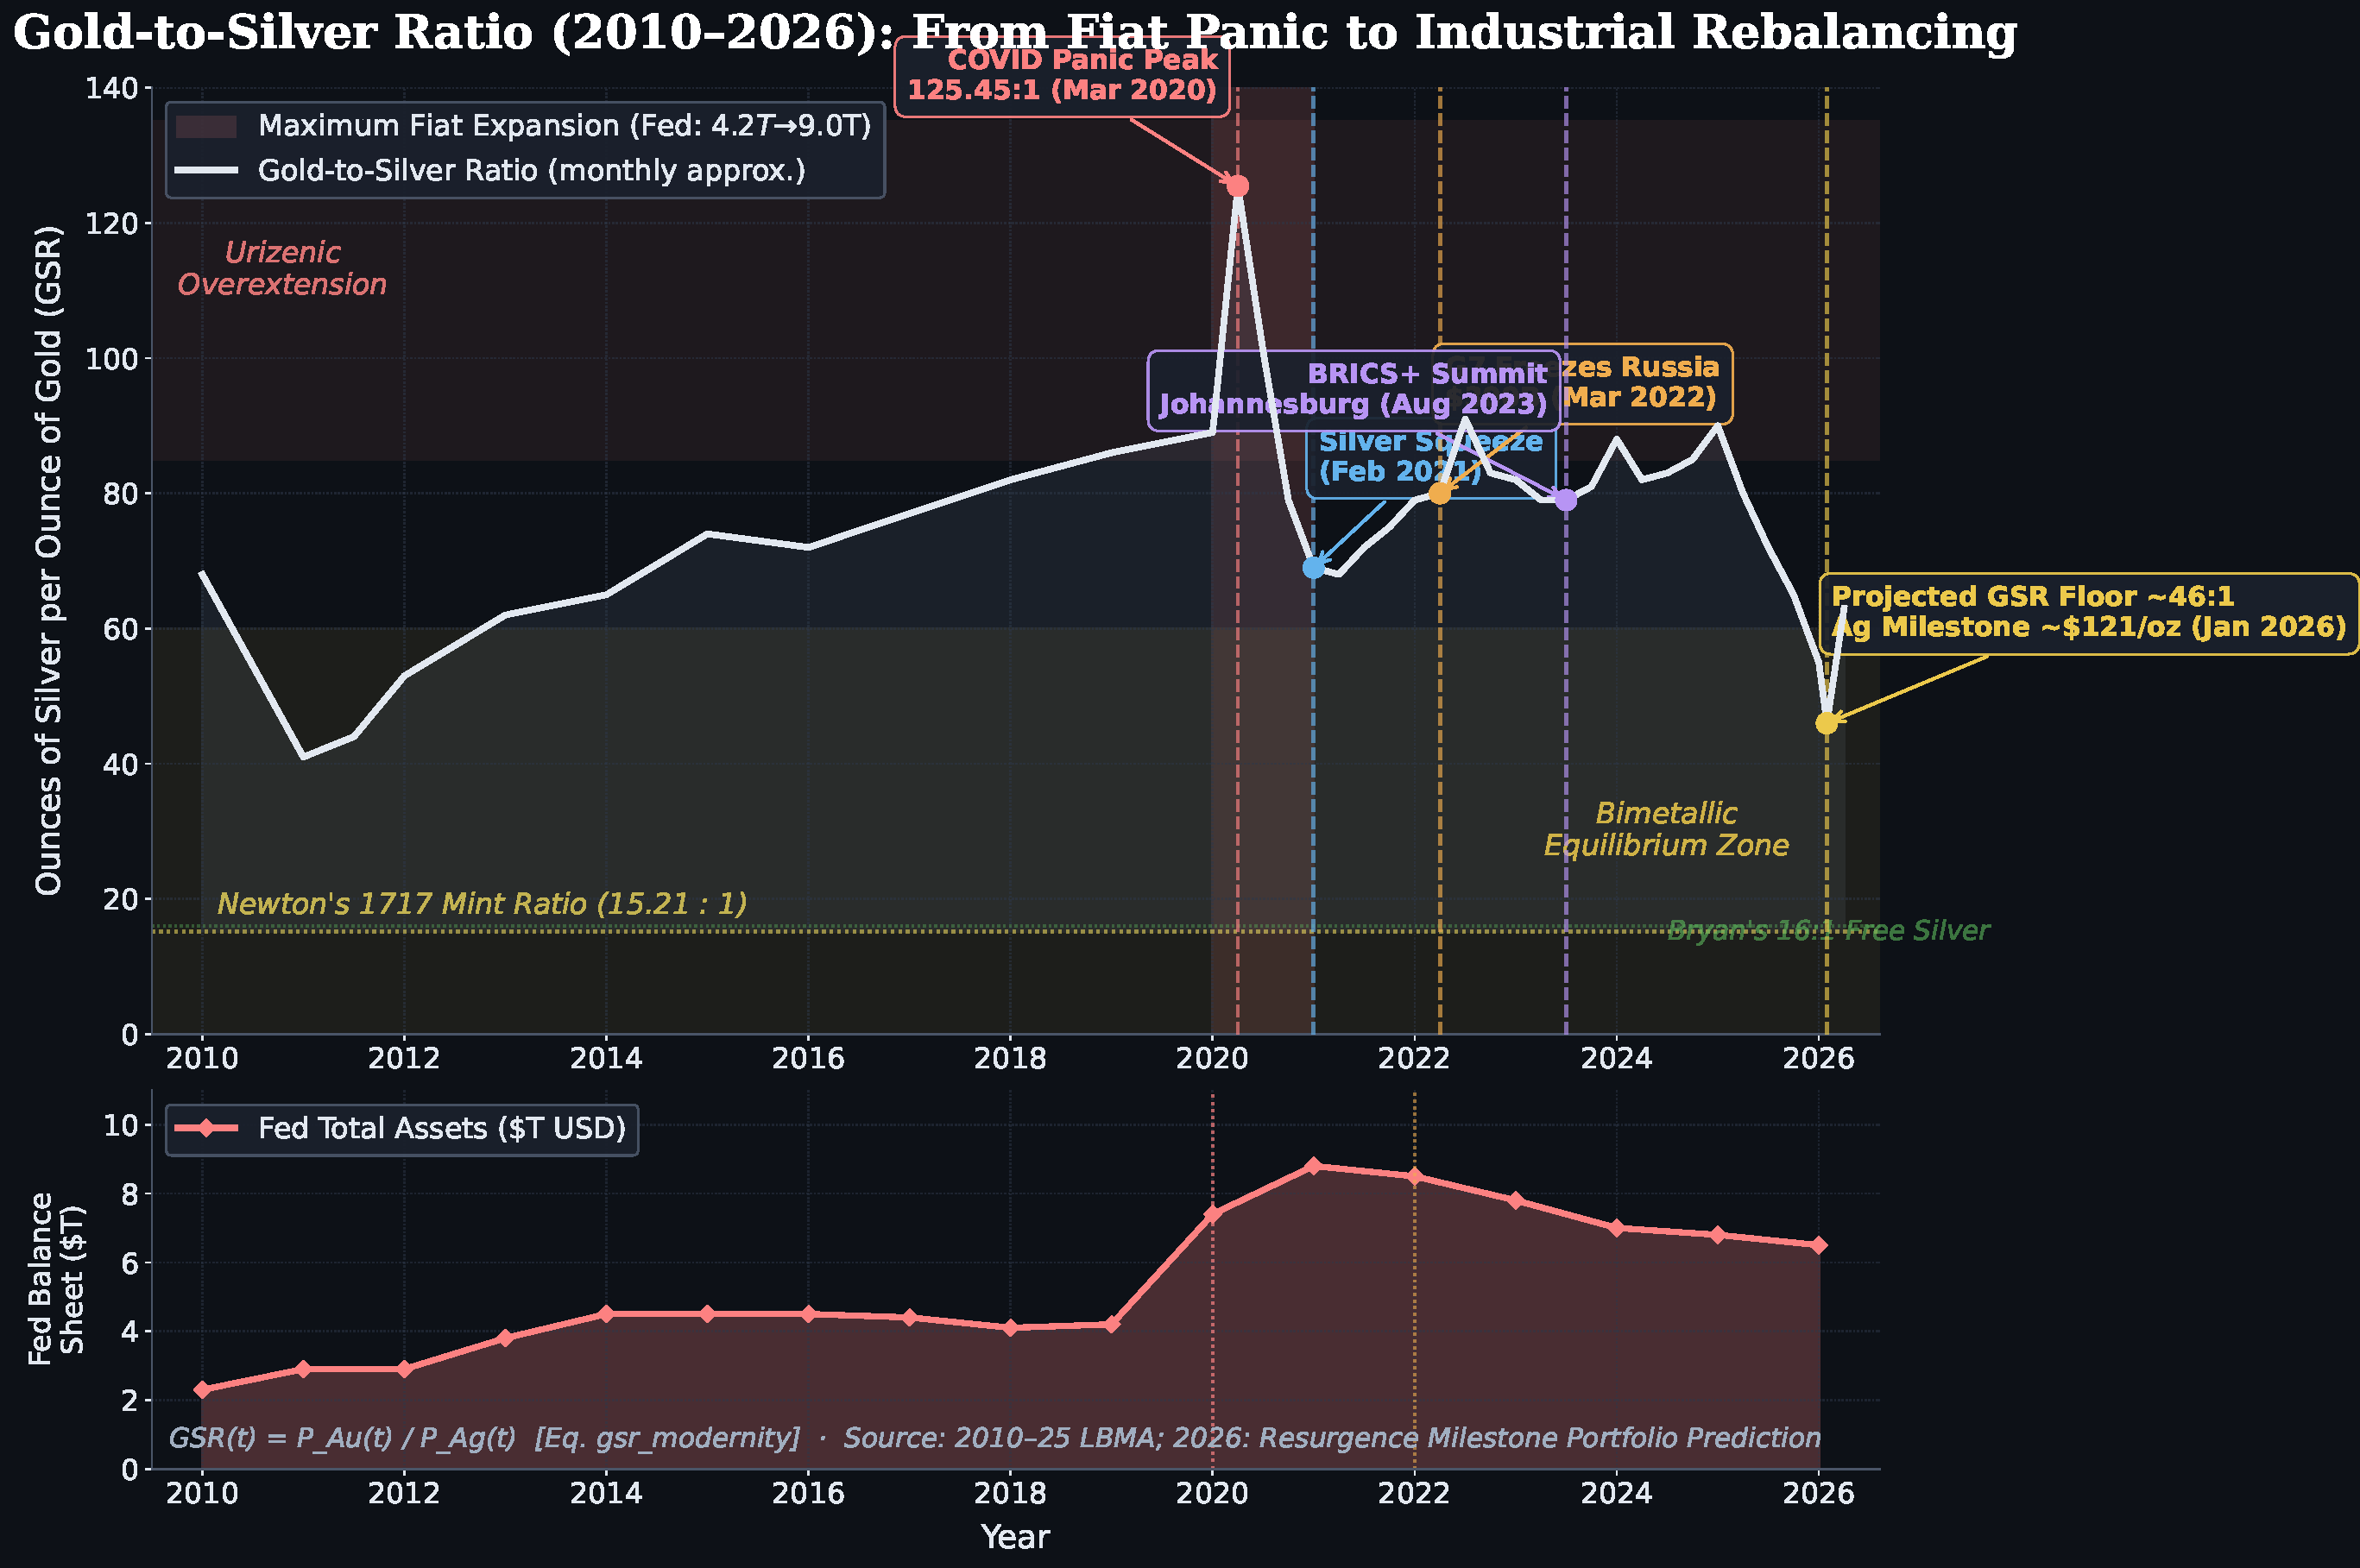
\includegraphics[keepaspectratio,alt={Gold-to-Silver Ratio and Fiat Expansion, 2010--2026. Top panel: empirical monthly gold-to-silver ratio (GSR, Eq. ) from 2010 through Q1 2026 plotting atomic gold and silver prices from the LBMA benchmark, with a dashed reference line plotting Bryan's historic 16:1 bimetallic target. Vertical markers denote structurally significant events: COVID liquidity panic peak near 127:1 (18 March 2020); Silver Squeeze coordination event (February 2021); G7 freezing of Russian reserves triggering central bank gold accumulation (March 2022); BRICS+ Johannesburg summit (August 2023); and silver nominal high with GSR floor below 50:1 (January 2026). Bottom panel: tracks the Federal Reserve Total Assets (\$T), visualizing the maximum Urizenic fiat expansion (\$4.2T \$8.9T) coinciding with peak precious metal volatility in 2020--2021. The systematic compression of the ratio from 125:1 toward 46:1 encodes the structural reassertion of silver's dual monetary-industrial demand against gold's sovereign safe-haven function.}]{../figures/gsr_contemporary_dark.pdf}}
\caption{Gold-to-Silver Ratio and Fiat Expansion, 2010--2026. Top panel:
empirical monthly gold-to-silver ratio (GSR, Eq. \ref{eq:gsr_modernity})
from 2010 through Q1 2026 plotting atomic gold and silver prices from
the LBMA benchmark, with a dashed reference line plotting Bryan's
historic 16:1 bimetallic target. Vertical markers denote structurally
significant events: COVID liquidity panic peak near 127:1 (18 March
2020); Silver Squeeze coordination event (February 2021); G7 freezing of
Russian reserves triggering central bank gold accumulation (March 2022);
BRICS+ Johannesburg summit (August 2023); and silver nominal high with
GSR floor below 50:1 (January 2026). Bottom panel: tracks the Federal
Reserve Total Assets (\$T), visualizing the maximum Urizenic fiat
expansion (\$4.2T \to \$8.9T) coinciding with peak precious metal
volatility in 2020--2021. The systematic compression of the ratio from
125:1 toward 46:1 encodes the structural reassertion of silver's dual
monetary-industrial demand against gold's sovereign safe-haven
function.}\label{fig-gsr-contemporary}
\end{figure}

\newpage

\section{Discussion: The Alchemical Forge and the Destruction of
Urizen}\label{discussion-the-alchemical-forge-and-the-destruction-of-urizen}

Human history operates by oscillating between periods of meta-stability
and thermodynamic collapse. The complete breakdown of the British
bimetallic standard---accelerated by the paper panic of 26 February
1797, debated during the Bullionist Controversy, finalized by the
establishment of the rigid gold anchor on 22 June 1816 (56 Geo. III
c.68), and later tightened by the 1844 Bank Charter Act and
ledger-credit expansion---is traditionally interpreted by orthodox
economic historians as a victory for empirical governance, stability,
and rationality over the anarchy of fluctuating bullion markets
\citep{fetter1965development}. As demonstrated in the preceding
transatlantic analysis, this trajectory was replicated in parallel
across the Atlantic: Hamilton's republican bimetallic ratio of 15:1
(1792) underwent the same Gresham-driven degradation, culminating in the
American ``Crime of 1873'', the fiat centralization of the 1971 Nixon
Shock, and the subsequent decentralized, state-level metallic rebellions
extending through 2026. This roughly three-century arc constitutes a
global confirmation of the Urizenic principle's expansion and Orc's
resistance. As we and others have explored, Blake's prophetic
epistemology anticipated this very arc: the cycle of revolution,
institutional reconsolidation, and renewed prophetic rupture that
characterizes the history of monetary sovereignty maps onto the
pragmatist architecture of inquiry itself---the organism encountering an
indeterminate situation, breaking inherited habit, and forging, through
fallibilistic self-correction, new modes of engagement with the world
\citep{friedman2026blake, friedman2026doors, laughlin1898bimetallism, blake1793america}.

\subsection{The Blakean Inversion of Traditional Neoclassical Economic
Orthodoxy}\label{the-blakean-inversion-of-traditional-neoclassical-economic-orthodoxy}

However, when this history is mapped against William Blake's prophetic
critiques, the financial historiography of Alexander Del Mar
\citep{delmar1895history}, and the dimensions of \emph{Fourfold Vision},
the usual neoclassical consolation narrative loses its force. The 1816
Coinage Act stands exposed not as the march of progress, but as a
regression back into the materialist, atomized despair of \emph{Single
Vision (Ulro)} \citep{redish1990evolution}. Setting the price of human
labor against geometric gold---the 22-carat sovereign at 123.274 grains,
minted with steam-powered precision on Boulton's presses---and
fictitious ``allegoric riches'' revives the miser logic of the Reynolds
marginalia explored earlier \citep{blake1808annotations}. The Mint has
triumphed over the Forge.

\subsection{The Double Bind of Metal and
Paper}\label{the-double-bind-of-metal-and-paper}

Blake recognized that standardizing vital human existence to finite,
atomized currency sets a course towards both spiritual and societal
entropy. The debate between the Bullionists and Anti-Bullionists was
ultimately a double bind: a choice between the idol of dead metal and
the idol of dead paper \citep{thornton1802nature, ricardo1810high}. From
a generic, first-principles standpoint, both positions share the same
axiom: that value is a \emph{quantity} to be measured rather than a
\emph{quality} to be cultivated. The Bullionists insist the measuring
rod must be gold---the post-1816 sovereign's 113 grains of fine gold;
the Anti-Bullionists accept paper as a sufficient proxy, backed only by
the Bank's sovereign guarantee and the ``needs of trade.'' Neither party
questions whether the act of measurement itself is the source of the
disease.

Blake grasped this deeper pattern. In \emph{The Book of Thel}, his
question---``Can Wisdom be put in a silver rod? / Or Love in a golden
bowl?'' (1789)---rejects the premise of both positions
\citep{blake1789thel}. Wisdom cannot be weighed; Love cannot be minted.
By interrogating the dualistic friction of bimetallism through the
creative furnace of Los---transmuting the isolated solar gold and lunar
silver into a Fourfold qualitative ontology through acts of artistic and
spiritual labor---Blake provides the template for human liberation
\citep{erdman1988complete, thompson1993witness}.

\subsection{Toward a Prophetic Economics: Active Inference and Fourfold
Refusal}\label{toward-a-prophetic-economics-active-inference-and-fourfold-refusal}

Under Active Inference, approximate Bayesian agents minimize an expected
free energy functional which decomposes into \textbf{pragmatic value}
(also known as constraint, or the cost of outcomes relative to prior
preferences) and \textbf{epistemic value} (the information gain from
resolving uncertainty about hidden causes)
\citep{friston2010free, parr2018anatomy}. Read alongside Blake's
monetary arc, that split suggests an \textbf{epistemic bimetallism}: a
living intelligence must keep both moments in tension---neither
collapsing into pure pragmatic fixation (the monometallic drive to
enforce a single, ``correct'' price and policy outcome at all costs) nor
dissolving into endless epistemic drift without commitments strong
enough to act. Bimetallism's statutory pairing of gold and silver is a
crude institutional image of the same structure: two incommensurable yet
co-constitutive registers of value that prevent the system from
pretending that one scalar solves the whole problem. Where Urizenic
finance demands a unique numéraire---gold \emph{or} paper, ledger
\emph{or} metal---Blake's Fourfold refusal and the free-energy formalism
both insist that viable cognition (and viable political economy)
requires coupling preference-respecting action with openness to evidence
that can falsify one's model of the world. Blake's ``doors of
perception'' can be formalized as statistical boundaries (Markov
blankets) separating self from world, and his ``fourfold vision'' maps
directly onto hierarchical precision-weighting across processing depths,
establishing epistemic balance
\citep{friedman2026blake, friedman2026doors}. Epistemic bimetallism is
therefore not a return to nineteenth-century coin ratios but a norm for
any system, biological or institutional, that would avoid both the
violence of Single Vision and the paralysis of unconstrained scepticism.

True wealth cannot be quantified by the gram, nor engineered by
``chimeric measurement'' regimes \citep{albernaz2024common}, nor secured
behind the doors of the Bank of England. It cannot be legislated by a
Newton or a Lord Liverpool, codified in a statute at 56 Geo. III c.68,
or guaranteed by whatever bullion happens to sit in the Bank's vaults.
As Blake anticipated the Marxist critique of alienation decades before
\emph{Das Kapital}, he recognized that reducing human life to capitalist
relations severs humanity from its creative essence. The Erdman reading
of Urizen, ``slave labor,'' and the ``great Work master'' as prefiguring
Marx's abstract labor was established in the Introduction
\citep{erdman1954prophet}.

The years 2020 to 2026 have revivified this prophetic frame in bullion
markets, retail coordination, industrial silver draw, sovereign gold
accumulation, reserve sanctions, and CBDC proliferation; the figures and
citations are consolidated in \hyperref[sec-spectral-2020-2026]{§ The
Spectral Made Tangible (2020--2026)}
\citep{worldgoldcouncil2024demand, eichengreen2022sanctions, atlanticcouncil2026cbdc, blake1794urizen}.

\subsection{The Temporal Grammar: Coherence, Rupture, and
Regeneration}\label{the-temporal-grammar-coherence-rupture-and-regeneration}

The epistemic bimetallism articulated above---the necessary tension
between pragmatic fixation and epistemic openness---has recently
received rigorous mathematical grounding through the
Coherence-Rupture-Regeneration (CRR) framework \citep{sabine2026doors}.
Sabine demonstrates that any bounded system governed by the Free Energy
Principle must oscillate through three coupled temporal phases, each of
which maps onto the Blakean mythological cycle with structural
precision.

\subsubsection{The Phase of Coherence: Los Laboring at the
Forge}\label{the-phase-of-coherence-los-laboring-at-the-forge}

The first phase is \emph{coherence}: the system accumulates Fisher-Rao
arc length on its statistical manifold. Each observation tightens the
posterior, each datum extends the geodesic the system has traversed. In
Blake's idiom, this is Los at the forge---each hammer-blow an increment
of evidence, each spark a datum binding the generative model more
tightly to its world. Coherence is not static equilibrium but
\emph{active construction}: the system builds, through sustained
engagement with its environment, the very manifold on which it will
eventually exhaust itself.

\subsubsection{The Phase of Rupture: Orc Breaking Urizen's Rigid
Chains}\label{the-phase-of-rupture-orc-breaking-urizens-rigid-chains}

The second phase is \emph{rupture}: the Dirac-delta transition triggered
when accumulated coherence saturates the manifold's geodesic extent.
Sabine formalises this threshold as:

\[C \cdot \Omega = 1\]

where \(C\) is accumulated coherence (Fisher-Rao arc length) and
\(\Omega\) is the manifold's total geodesic capacity. At saturation, the
system can no longer assimilate new evidence within its current
geometry---the model \emph{breaks}. In Blake's prophecy, this is Orc
breaking Urizen's chains: the revolutionary eruption that shatters a
regime grown too rigid to accommodate the living world it purports to
govern.

\subsubsection{The Phase of Regeneration: Albion Rising from the
Ashes}\label{the-phase-of-regeneration-albion-rising-from-the-ashes}

The third phase is \emph{regeneration}: the exponentially weighted
reconstruction from historical memory. The system does not restart from
nothing; it reconstitutes from a kernel that preserves the most salient
features of prior experience while discarding the exhausted geometry.
This is Albion rising---the Universal Man reassembling from the
fragments of the fallen Zoas, the kernel reopening.

\subsubsection{\texorpdfstring{Topological Invariants and the
Theoretical Necessity of the \(\sqrt{2}\)
Ratio}{Topological Invariants and the Theoretical Necessity of the \textbackslash sqrt\{2\} Ratio}}\label{topological-invariants-and-the-theoretical-necessity-of-the-sqrt2-ratio}

Two symmetry classes yield parameter-free thresholds fixed by manifold
topology alone:

\begin{itemize}
\tightlist
\item
  \(\pi) for \(\mathbb{Z}_2\) symmetry (bistable, sensory): the
  boundary alternation at every edge of a Markov blanket.
\item
  \(2\pi) for \(\mathrm{SO}(2)\) symmetry (rotational, prior-bearing):
  the continuous belief cycle at every node.
\end{itemize}

Their ratio is exactly 2---a topological invariant that is, as Sabine
observes, structurally identical to the Cramér-Rao bound, the
Mandelstam-Tamm quantum speed limit, and the Higgs vacuum manifold. The
CRR finding that the free-energy-optimal precision allocation between
sensory and prior channels satisfies:

\[\frac{\pi_p}{\pi_s} = \sqrt{2}\]

gives quantitative substance to our epistemic bimetallism. Viable
cognition, and viable political economy, requires not merely \emph{two}
registers of value but their maintenance at a specific, mathematically
determined ratio \citep{sabine2026doors, friston2010free}.

The Urizenic collapse from bimetallism to monometallism can be modeled
an \(\Omega\)-collapse---the regeneration kernel sharpening until only
the most familiar patterns (geometric gold, single numéraire, Newton's
sleep) reconstitute. The Orcian ruptures traced across three
centuries---the Bank Restriction of 1797, Bryan's Cross of Gold, the
Nixon Shock, the state-level metallic rebellions of 2011--2026---are
threshold-crossings at which accumulated coherence exhausted its
regime's finite capacity and the system was forced to reorganise.

Blake's ``Without Contraries is no progression'' is, in CRR's
information geometry, a theorem \citep{blake1790marriage}. The Forge
does not merely resist the Mint; it regenerates, on a manifold whose
curvature is set by the very topology of bounded cognition, the capacity
for renewed vision that every monometallic collapse temporarily
annihilates. The conclusion states, without repeating the formalism,
what is at stake when that regenerative capacity meets the monetary
forms of the present.

\newpage

\section{Conclusion: The Eternal Stance of the Forge Against the
Mint}\label{conclusion-the-eternal-stance-of-the-forge-against-the-mint}

The transition from bimetallism to the gold standard---and ultimately to
unanchored twentieth-century fiat, and now to programmable digital
currency---was not merely an economic sequence, but the successive
enforcement of spiritual abstractions. The
coherence--rupture--regeneration temporal grammar implies that each of
these monetary regimes advanced until its own geometry could absorb no
more lived contradiction. Epistemic bimetallism is therefore less a
policy prescription than a refusal to let any one single
abstraction---bullion weight, bank ledger, or executable token---stand
in for the full fourfold valuation of persons in community.

Blake's final prophetic vision---the building of Jerusalem ``Among these
dark Satanic Mills'' (\emph{Milton}, Preface, Plate 1; Erdman p.~95)
\citep{erdman1988complete}---is a transfiguration of economic reality
and economy: the insistence that the human community can and must create
systems of value that honor the irreducible dignity of every living
soul.

Programmable retail CBDC architectures and state-level reassertions of
Article I's metallic mandate are rival institutional imaginations of the
same enclosed metric; neither is destiny, and both can be read as
increasingly desparate attempts to answer Orc with a tighter Urizenic
grid. These forces operate with copper acid-baths, blockchains, private
ledgers, legislative chambers, and surely other tools to come. Against
this single vision, the human imperative remains identical:
energetically resist the geometric reduction of human life to a metric,
to maintain minimum two (minimum!), and assert the openly infinite
valuation of the human form and imagination. Los hammers at the anvil of
every century; the Forge stands eternal against the Mint.



\clearpage

\bibliography{references}
\end{document}
